% Capitolul 10: Ipoteza Pieței Fractale (FMH) — versiunea v2 restructurată
% Statistica Piețelor Financiare
% Program de licență, Academia de Studii Economice din București

\documentclass[9pt, aspectratio=169, t, handout]{beamer}

\setbeamersize{text margin left=8mm, text margin right=8mm}

%=============================================================================
% TEMĂ ȘI STIL
%=============================================================================
\usetheme{default}

\definecolor{MainBlue}{RGB}{26, 58, 110}
\definecolor{AccentBlue}{RGB}{26, 58, 110}
\definecolor{IDAred}{RGB}{205, 0, 0}
\definecolor{DarkGray}{RGB}{51, 51, 51}
\definecolor{MediumGray}{RGB}{128, 128, 128}
\definecolor{LightGray}{RGB}{248, 248, 248}
\definecolor{VeryLightGray}{RGB}{235, 235, 235}
\definecolor{KeynoteGray}{RGB}{218, 218, 218}
\definecolor{SectionGray}{RGB}{120, 120, 120}
\definecolor{FooterGray}{RGB}{100, 100, 100}
\definecolor{Crimson}{RGB}{220, 53, 69}
\definecolor{Forest}{RGB}{46, 125, 50}
\definecolor{Amber}{RGB}{181, 133, 63}
\definecolor{Orange}{RGB}{230, 126, 34}
\definecolor{Purple}{RGB}{142, 68, 173}

\setbeamertemplate{background}{%
    \begin{tikzpicture}[remember picture, overlay]
        \shade[shading=axis, shading angle=315,
        top color=LightGray, bottom color=KeynoteGray]
        (current page.south west) rectangle (current page.north east);
    \end{tikzpicture}%
}
\setbeamercolor{background canvas}{bg=}

\setbeamercolor{palette primary}{bg=MainBlue, fg=white}
\setbeamercolor{palette secondary}{bg=MainBlue!85, fg=white}
\setbeamercolor{palette tertiary}{bg=MainBlue!70, fg=white}
\setbeamercolor{structure}{fg=MainBlue}
\setbeamercolor{title}{fg=IDAred}
\setbeamercolor{frametitle}{fg=IDAred, bg=}
\setbeamercolor{block title}{bg=MainBlue, fg=white}
\setbeamercolor{block body}{bg=VeryLightGray, fg=DarkGray}
\setbeamercolor{block title alerted}{bg=Crimson, fg=white}
\setbeamercolor{block body alerted}{bg=Crimson!8, fg=DarkGray}
\setbeamercolor{block title example}{bg=Forest, fg=white}
\setbeamercolor{block body example}{bg=Forest!8, fg=DarkGray}
\setbeamercolor{item}{fg=MainBlue}

\setbeamercolor{author in head/foot}{fg=FooterGray, bg=}
\setbeamercolor{title in head/foot}{fg=FooterGray, bg=}
\setbeamercolor{date in head/foot}{fg=FooterGray, bg=}
\setbeamercolor{section in head/foot}{fg=FooterGray, bg=}
\setbeamercolor{subsection in head/foot}{fg=FooterGray, bg=}

\setbeamertemplate{itemize item}{\color{MainBlue}$\boxdot$}
\setbeamertemplate{itemize subitem}{\color{MainBlue}$\blacktriangleright$}
\setbeamertemplate{itemize subsubitem}{\color{MainBlue}\tiny$\bullet$}
\setbeamertemplate{itemize/enumerate body begin}{\normalsize}
\setbeamertemplate{itemize/enumerate subbody begin}{\normalsize}

\setlength{\leftmargini}{10pt}
\setlength{\leftmarginii}{10pt}
\makeatletter
\def\@listi{\leftmargin\leftmargini \topsep 0pt \parsep 0pt \itemsep 0pt}
\def\@listii{\leftmargin\leftmarginii \topsep 0pt \parsep 0pt \itemsep 0pt}
\makeatother

\setbeamertemplate{navigation symbols}{}

%=============================================================================
% ANTET
%=============================================================================
\setbeamertemplate{headline}{%
    \vskip10pt%
    \hbox to \paperwidth{%
        \hskip0.5cm%
        {\small\color{FooterGray}\thesection.\ \renewcommand{\hyperlink}[2]{##2}\insertsectionhead}%
        \hfill%
        \showlevel\hspace{4pt}%
        \textcolor{FooterGray}{\small\insertframenumber}%
        \hskip0.5cm%
    }%
    \vskip4pt%
    {\color{\currentlevelcolor}\hrule height 1.5pt}%
    \global\slidelevelnum=0%
    \gdef\currentlevelcolor{FooterGray}%
}

%=============================================================================
% SUBSOL
%=============================================================================
\usepackage{fontawesome5}

\setbeamertemplate{footline}{%
    {\color{FooterGray}\hrule height 0.4pt}%
    \vskip4pt%
    \hbox to \paperwidth{%
        \hskip0.5cm%
        \textcolor{FooterGray}{\small Statistica Piețelor Financiare}%
        \hfill%
        \raisebox{-0.1em}{%
            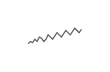
\begin{tikzpicture}[x=0.08em, y=0.08em, line width=0.4pt]
                \draw[FooterGray] (0,3) -- (1,4) -- (2,3.5) -- (3,5) -- (4,4) -- (5,6) -- (6,5.5) -- (7,4) -- (8,5) -- (9,7) -- (10,6) -- (11,5) -- (12,6.5) -- (13,8) -- (14,7) -- (15,6) -- (16,7.5) -- (17,9) -- (18,8) -- (19,7) -- (20,8.5) -- (21,10) -- (22,9) -- (23,8) -- (24,9.5);
            \end{tikzpicture}%
        }%
        \hskip0.5cm%
    }%
    \vskip6pt%
}

%=============================================================================
% PACHETE
%=============================================================================
\usepackage[utf8]{inputenc}
\usepackage[T1]{fontenc}
\usepackage{amsmath, amssymb, amsthm}
\usepackage{mathtools}
\usepackage{bm}
\usepackage{tikz}
\usetikzlibrary{arrows.meta, positioning, shapes, calc, decorations.pathreplacing, shadings}
\usepackage{booktabs}
\usepackage{multirow}
\usepackage{array}
\usepackage{graphicx}
\usepackage{hyperref}
\usepackage{colortbl}
\usepackage{pifont}
\usepackage{listings}
\lstset{language=Python, basicstyle=\ttfamily\scriptsize, keywordstyle=\color{MainBlue}\bfseries,
  commentstyle=\color{Forest}, stringstyle=\color{Crimson}, breaklines=true,
  frame=none, backgroundcolor=\color{VeryLightGray}, xleftmargin=2mm}
\hypersetup{colorlinks=true, linkcolor=MainBlue, urlcolor=MainBlue}
\graphicspath{{../../logos/}{../../charts/}{../../photos/}}
\hfuzz=0.5pt
\vfuzz=0.5pt

%=============================================================================
% COMANDA QUANTLET
%=============================================================================
\newcommand{\quantlet}[2]{%
    \vspace{-0.25cm}%
    \hfill\href{#2}{%
        \raisebox{-0.15em}{
\includegraphics[height=0.7em]{ql_logo.png}}%
        \textcolor{MainBlue}{\tiny\ #1}%
    }\par%
}

\newcommand{\figql}[2]{%
    {\centering\href{#2}{%
        \raisebox{-0.15em}{
\includegraphics[height=0.6em]{ql_logo.png}}%
        \textcolor{MainBlue}{\tiny\ #1}%
    }\par}%
}

%=============================================================================
% PAGINĂ TITLU
%=============================================================================
\defbeamertemplate*{title page}{hybrid}[1][]
{
    \vspace{0.2cm}
    \begin{center}
        \href{https://www.ase.ro}{
\includegraphics[height=1.0cm]{ase_logo.png}}\hspace{0.3cm}%
        \href{https://theida.net}{
\includegraphics[height=1.0cm]{ida_logo.png}}\hspace{0.3cm}%
        \href{https://blockchain-research-center.com}{
\includegraphics[height=1.0cm]{brc_logo.png}}\hspace{0.3cm}%
        \href{https://www.ai4efin.ase.ro}{
\includegraphics[height=1.0cm]{ai4efin_logo.png}}\hspace{0.3cm}%
        \href{https://ipe.ro/new}{
\includegraphics[height=1.0cm]{acad_logo.png}}\hspace{0.3cm}%
        \href{https://www.digital-finance-msca.com}{
\includegraphics[height=1.0cm]{msca_logo.png}}%
    \end{center}

    \vspace{0.6cm}

    \begin{center}
        \begin{minipage}{0.1\textwidth}
            \centering
            \href{https://quantlet.com}{
\includegraphics[height=1.1cm]{ql_logo.png}}
        \end{minipage}%
        \begin{minipage}{0.78\textwidth}
            \centering
            {\LARGE\bfseries\usebeamercolor[fg]{title}\inserttitle}

            \vspace{0.3cm}

            {\usebeamerfont{subtitle}\usebeamercolor[fg]{title}\insertsubtitle}
        \end{minipage}%
        \begin{minipage}{0.1\textwidth}
            \centering
            \href{https://quantinar.com}{
\includegraphics[height=1.1cm]{qr_logo.png}}
        \end{minipage}
    \end{center}

    \vspace{0.6cm}

    \hspace{0.5cm}\begin{minipage}[t]{0.9\textwidth}
        \usebeamerfont{author}\insertauthor
    \end{minipage}

    \vspace{0.3cm}

    \hspace{0.5cm}\begin{minipage}[t]{0.9\textwidth}
        \raggedright\small\insertinstitute
    \end{minipage}
}

%=============================================================================
% MEDII PENTRU TEOREME
%=============================================================================
\theoremstyle{definition}
\setbeamertemplate{theorems}[numbered]
\newtheorem{defn}{Definiție}
\newtheorem{thm}{Teoremă}
\newtheorem{prop}{Propoziție}
\newtheorem{rmk}{Observație}

\newenvironment{cminipage}[1]{%
    \par\noindent\hfill\begin{minipage}{#1}\ignorespaces
}{%
    \end{minipage}\hfill\null\par
}

%=============================================================================
% COMENZI PERSONALIZATE
%=============================================================================
\newcommand{\E}{\mathbb{E}}
\newcommand{\Var}{\text{Var}}
\newcommand{\Cov}{\text{Cov}}
\newcommand{\Corr}{\text{Corr}}
\newcommand{\R}{\mathbb{R}}
\newcommand{\N}{\mathbb{N}}
\newcommand{\Z}{\mathbb{Z}}
\newcommand{\B}{\mathbf{B}}
\newcommand{\imark}{\textcolor{MainBlue}{\textbullet}}

\newcount\slidelevelnum
\global\slidelevelnum=0
\makeatletter
\newcommand{\slidelevel}[1]{%
    \global\slidelevelnum=0%
    \def\tmp@SL{#1}\def\tmp@SLy{Y3}\def\tmp@SLm{MSc}\def\tmp@SLp{PhD}%
    \ifx\tmp@SL\tmp@SLy \global\slidelevelnum=1\fi%
    \ifx\tmp@SL\tmp@SLm \global\slidelevelnum=2\fi%
    \ifx\tmp@SL\tmp@SLp \global\slidelevelnum=3\fi%
}
\makeatother
\gdef\currentlevelcolor{FooterGray}
\newcommand{\showlevel}{%
    \ifnum\slidelevelnum=1%
        \colorbox{Forest}{\strut\textcolor{white}{\sffamily\bfseries\fontsize{8}{9}\selectfont Y3}}%
        \gdef\currentlevelcolor{Forest}%
    \fi%
    \ifnum\slidelevelnum=2%
        \colorbox{MainBlue}{\strut\textcolor{white}{\sffamily\bfseries\fontsize{8}{9}\selectfont MSc}}%
        \gdef\currentlevelcolor{MainBlue}%
    \fi%
    \ifnum\slidelevelnum=3%
        \colorbox{Crimson}{\strut\textcolor{white}{\sffamily\bfseries\fontsize{8}{9}\selectfont PhD}}%
        \gdef\currentlevelcolor{Crimson}%
    \fi%
    \ifnum\slidelevelnum=0%
        \gdef\currentlevelcolor{FooterGray}%
    \fi%
}

%=============================================================================
% INFORMAȚII TITLU
%=============================================================================
\title[Statistica Piețelor Financiare]{Statistica Piețelor Financiare}
\subtitle{Capitolul 10: Ipoteza Pieței Fractale (FMH)}
\author[D.T. Pele, A. Amza]{\texorpdfstring{\begin{tabular}[t]{@{}l@{}}Daniel Traian PELE \\ Antoaneta Amza\end{tabular}}{Daniel Traian PELE, Antoaneta Amza}}
\institute{Academia de Studii Economice din București\\
IDA Institute Digital Assets\\
Blockchain Research Center\\
AI4EFin Artificial Intelligence for Energy Finance\\
Academia Română, Institutul de Prognoză Economică\\
MSCA Digital Finance}
\date{}

\begin{document}

% Pagina de titlu
{
\setbeamertemplate{headline}{}
\setbeamertemplate{footline}{}
\begin{frame}
    \titlepage
\end{frame}
}

%=============================================================================
% OBIECTIVE DE ÎNVĂȚARE
%=============================================================================
\slidelevel{Y3}
\begin{frame}[shrink=15]{Obiective de învățare (Learning Objectives)}
\begin{cminipage}{0.95\textwidth}
\begin{block}{La finalul acestui capitol, veți fi capabili să:}
\begin{enumerate}
    \item[\textcolor{MainBlue}{\textbf{1.}}] \textbf{Identificați} limitele Ipotezei Pieței Eficiente (Efficient Market Hypothesis, EMH) și motivele pentru care e nevoie de un cadru fractal
    \item[\textcolor{MainBlue}{\textbf{2.}}] \textbf{Recunoașteți} obiectele fractale (Mandelbrot, Julia) și fractalii din natură
    \item[\textcolor{MainBlue}{\textbf{3.}}] \textbf{Definiți} autosimilaritatea statistică și dimensiunea fractală (box-counting)
    \item[\textcolor{MainBlue}{\textbf{4.}}] \textbf{Estimați} exponentul Hurst $H$ prin analiza R/S (Rescaled Range) și DFA (Detrended Fluctuation Analysis)
    \item[\textcolor{MainBlue}{\textbf{5.}}] \textbf{Interpretați} rezultatele empirice pe acțiuni, cripto, FX (Foreign Exchange)
    \item[\textcolor{MainBlue}{\textbf{6.}}] \textbf{Aplicați} mișcarea browniană fracționară (fractional Brownian motion, fBm) pentru memorie lungă
    \item[\textcolor{MainBlue}{\textbf{7.}}] \textbf{Discutați} multifractalitatea, MMAR (Multifractal Model of Asset Returns) și implicațiile pentru risk management
    \item[\textcolor{MainBlue}{\textbf{8.}}] \textbf{Analizați} studii de caz: 1987, 2008, COVID-19, BVB (Bursa de Valori București, Bucharest Stock Exchange), Bitcoin
\end{enumerate}
\end{block}
\end{cminipage}
\end{frame}

%=============================================================================
% CUPRINS
%=============================================================================
{
\setbeamertemplate{headline}{%
    \vskip10pt%
    \hbox to \paperwidth{\hskip0.5cm\hfill\hskip0.5cm}%
    \vskip4pt%
    {\color{FooterGray}\hrule height 0.4pt}%
}
\begin{frame}{}
    {\color{FooterGray}\hrule height 0.4pt}
    \vspace{0.1cm}
    {\Large\textcolor{IDAred}{\textbf{Cuprins}}}
    \vspace{0.2cm}
    {\small
    \begin{columns}[T]
        \begin{column}{0.48\textwidth}
            \begin{enumerate}
                \item De la EMH la FMH
                \item Fractali și scalare: intuiția
                \item Autosimilaritate și dimensiune fractală
                \item Exponentul Hurst
                \item Estimarea lui $H$: R/S și DFA
            \end{enumerate}
        \end{column}
        \begin{column}{0.48\textwidth}
            \begin{enumerate}\setcounter{enumi}{5}
                \item fBm și multifractalitate
                \item Aplicații empirice: crize, BVB, Bitcoin
                \item Implicații pentru managementul riscului
                \item Concluzii și întrebări de examen
            \end{enumerate}
            \vspace{0.15cm}
            {\scriptsize\textit{Anexe: A. Mandelbrot/Julia; B. Fractali în natură; C. Cod Python complet; D. Demonstrații, tabele și referințe extinse.}}
        \end{column}
    \end{columns}
    }
\end{frame}
}

%#############################################################################
\section{De la EMH la FMH}
%#############################################################################

\slidelevel{Y3}
\begin{frame}{Ce învățăm aici și de ce contează în finanțe?}
\begin{cminipage}{0.95\textwidth}
\begin{block}{Obiectivele §1}
\begin{itemize}\setlength{\itemsep}{2pt}
    \item Vedem \textbf{de ce EMH (Cap.~4) nu explică} crahurile, cozile grele și memoria lungă
    \item Introducem \textbf{Ipoteza Pieței Fractale} (Fractal Market Hypothesis, FMH, Peters 1991, 1994) ca cadru complementar
    \item Definim \textbf{diversitatea orizonturilor} și ce înseamnă \textbf{colapsul orizonturilor}
    \item Punte spre Cap.~4 (EMH) și Cap.~2 (cozi grele, distribuții stabile)
\end{itemize}
\end{block}
\end{cminipage}
\end{frame}

\slidelevel{Y3}
\begin{frame}[shrink=10]{De ce avem nevoie de o nouă paradigmă?}
\begin{cminipage}{0.95\textwidth}
\begin{columns}[T]
\begin{column}{0.55\textwidth}
\begin{itemize}\setlength{\itemsep}{2pt}
    \item \textbf{Eșecuri empirice ale EMH} (Cap.~4):
    \begin{itemize}\setlength{\itemsep}{0pt}
        \item Cozi grele: $\Pr(|r_t|>x)\gg\Phi(-x)$
        \item Volatility clustering: $\Corr(|r_t|,|r_{t+k}|)>0$
        \item Memorie lungă: $\rho(k)\sim Ck^{2H-2}$, $H>0{,}5$
        \item Crah-uri: 1987, 2008, COVID-2020
    \end{itemize}
    \item Sub gaussianitate: $\Pr(r\leq -22{,}6\%)\approx 10^{-50}$
    \item Mandelbrot (1963): bumbacul are \textit{varianță infinită}
\end{itemize}
\end{column}
\begin{column}{0.42\textwidth}
\centering
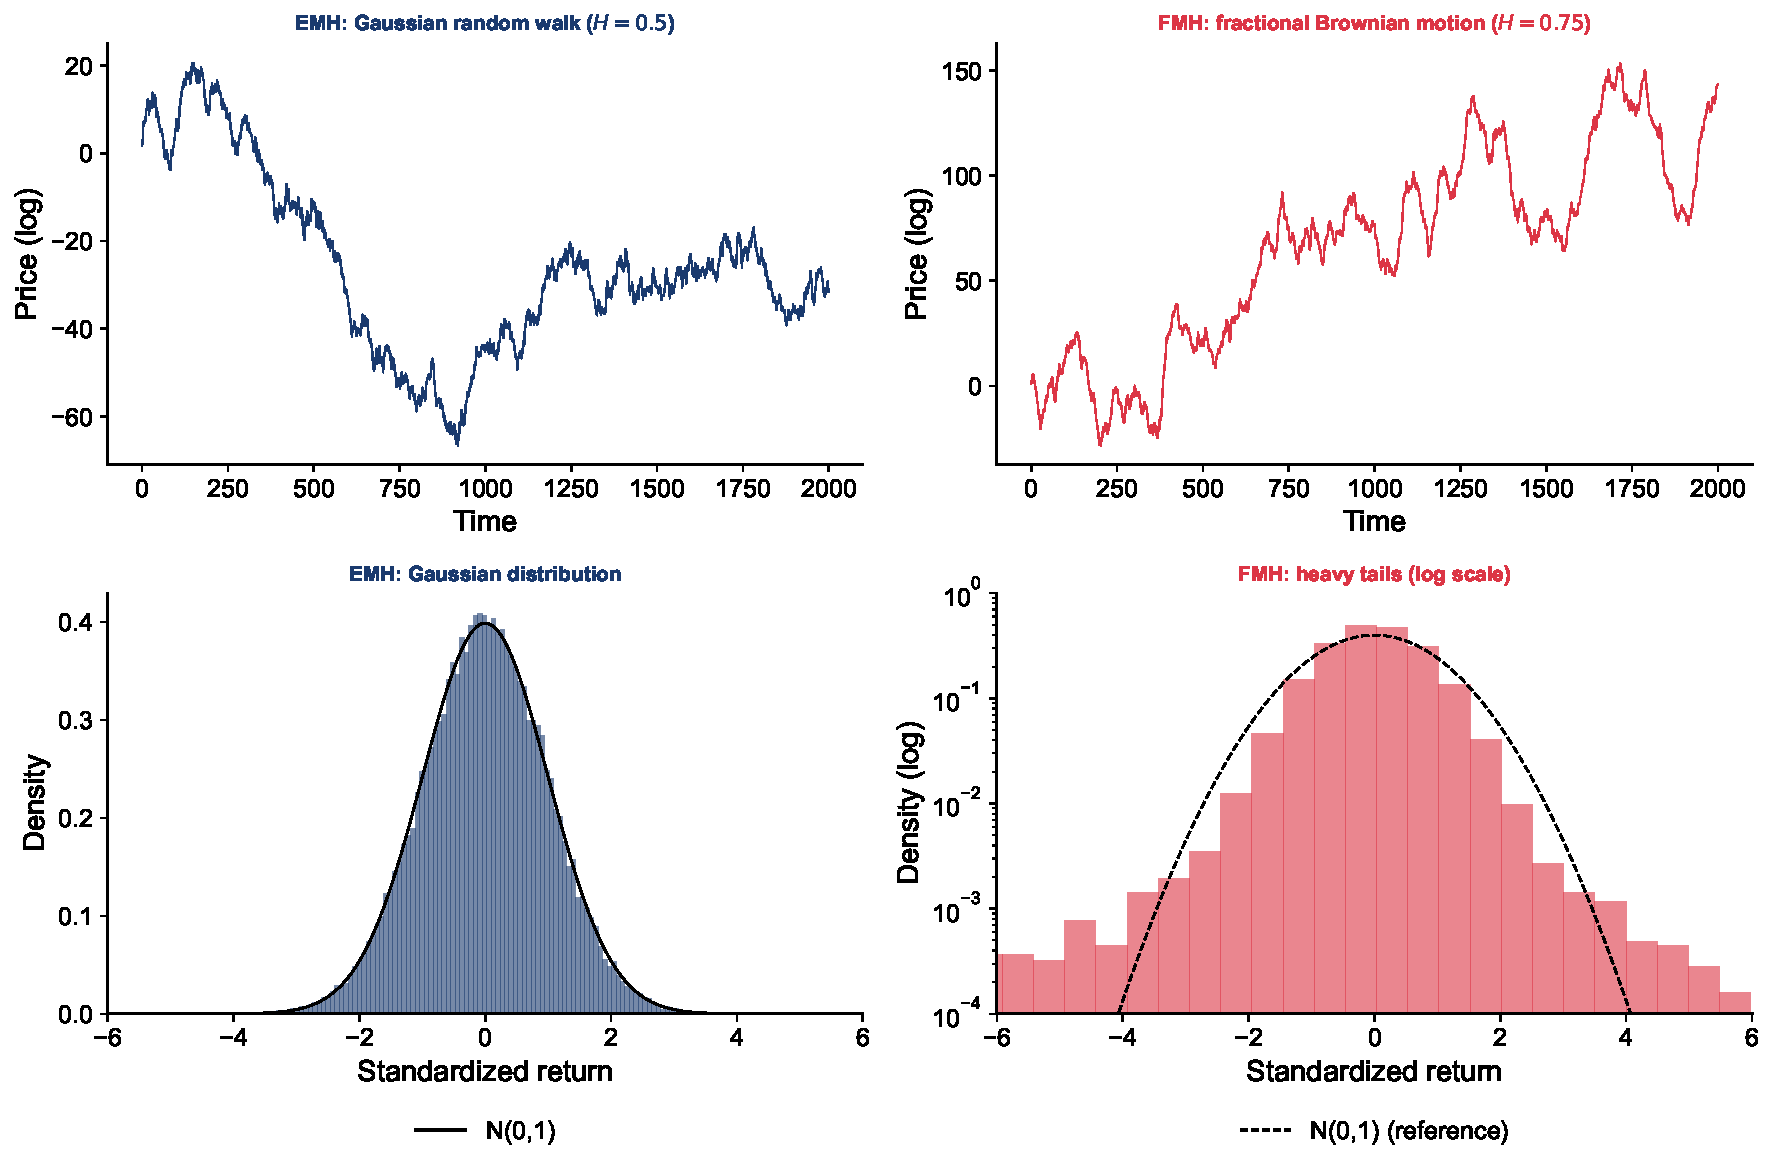
\includegraphics[width=\linewidth]{ch_fmh_emh_vs_fmh.pdf}
{\scriptsize\textcolor{MediumGray}{\textit{EMH (gaussian) vs FMH (fBm $H=0{,}75$); coadă subțire vs coadă grea.}}}
\figql{SFM\_ch\_fmh\_fractals: emh\_vs\_fmh}{https://github.com/danpele/SFM/tree/main/Quantlets/SFM_ch_fmh}
\end{column}
\end{columns}
\end{cminipage}
\end{frame}

\slidelevel{Y3}
\begin{frame}{Răspunsul FMH (Peters, 1991, 1994)}
\begin{cminipage}{0.95\textwidth}
\begin{block}{Trei principii FMH}
\begin{itemize}\setlength{\itemsep}{2pt}
    \item Piețele sunt sisteme \textbf{fractale}: structură statistică similară pe scale temporale diferite
    \item Investitorii operează pe \textbf{orizonturi multiple}: de la milisecunde (HFT) la decenii (pensii)
    \item Stabilitatea $\Leftrightarrow$ \textbf{diversitatea} orizonturilor; colapsul lor $\Rightarrow$ criză
\end{itemize}
\end{block}
\begin{exampleblock}{Inline gloss --- fBm}
\begin{itemize}\setlength{\itemsep}{0pt}
    \item fBm = mișcare browniană fracționară (Mandelbrot--Van~Ness, 1968)
    \item Generalizare a \textbf{mișcării browniene} cu memorie reglată de exponentul Hurst $H$
    \item $H=0{,}5$ recuperează \textbf{mișcarea browniană standard}; \textbf{definiție formală în §6}
\end{itemize}
\end{exampleblock}
\end{cminipage}
\end{frame}

\slidelevel{Y3}
\begin{frame}[shrink=10]{De la geometria euclidiană la fractali (Mandelbrot)}
\begin{cminipage}{0.95\textwidth}
\begin{columns}[T]
\begin{column}{0.50\textwidth}
\begin{block}{Geometria euclidiană}
\begin{itemize}\setlength{\itemsep}{0pt}
    \item \textbf{Forme}
    \begin{itemize}\setlength{\itemsep}{0pt}
        \item Regulate, netede
        \item Drepte, cercuri, sfere
    \end{itemize}
    \item \textbf{Dimensiune}
    \begin{itemize}\setlength{\itemsep}{0pt}
        \item $D\in\{0,1,2,3\}$ (întregi)
    \end{itemize}
\end{itemize}
\end{block}
\begin{block}{Geometria fractală (Mandelbrot, 1975)}
\begin{itemize}\setlength{\itemsep}{0pt}
    \item \textbf{Forme}
    \begin{itemize}\setlength{\itemsep}{0pt}
        \item Neregulate, fragmentate, autosimilare
        \item Țărmuri, nori, copaci, randamente
    \end{itemize}
    \item \textbf{Dimensiune}
    \begin{itemize}\setlength{\itemsep}{0pt}
        \item $D\in\R$ (fracționară)
    \end{itemize}
\end{itemize}
\end{block}
\end{column}
\begin{column}{0.46\textwidth}
\begin{center}
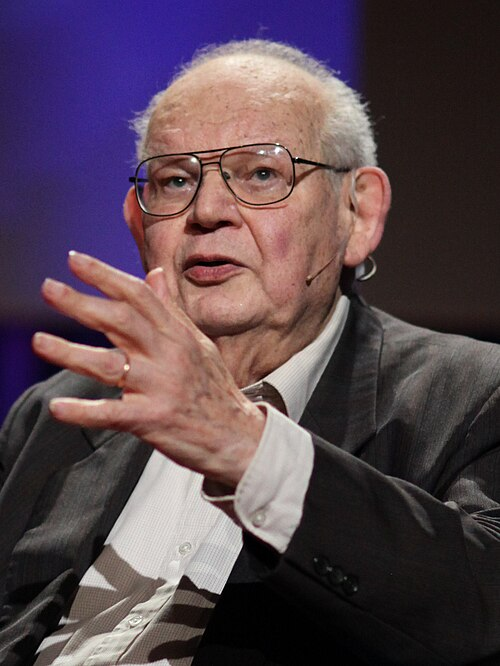
\includegraphics[height=2.4cm,keepaspectratio]{mandelbrot.jpg}\\[1pt]
{\scriptsize\textcolor{MediumGray}{\textbf{Benoît Mandelbrot} (1924--2010)}}
\end{center}
\begin{alertblock}{Citat (Mandelbrot, 1982)}
\begin{itemize}\setlength{\itemsep}{0pt}
    \item \textit{,,Norii nu sunt sfere''}
    \item \textit{,,Țărmurile nu sunt cercuri''}
    \item \textit{,,Fulgerul nu călătorește în linie dreaptă''}
\end{itemize}
\end{alertblock}
\end{column}
\end{columns}
\end{cminipage}
\end{frame}

\slidelevel{Y3}
\begin{frame}[shrink=10]{Anomalii care contrazic EMH}
\begin{cminipage}{0.95\textwidth}
\renewcommand{\arraystretch}{1.2}
\begin{center}
\small
\begin{tabular}{ll}
\toprule
\textbf{Anomalie} & \textbf{Predicție EMH} \\
\midrule
Cozi grele & Imposibil sub gaussianitate \\
Volatility clustering & Independență $\Rightarrow$ corelație 0 \\
Memorie lungă, $\rho(k)\sim k^{2H-2}$, $H>0{,}5$ & $\rho(k)=0$ pentru $k>0$ \\
Momentum (3--12 luni) & Imposibil sub mers aleator \\
Reversal (3--5 ani) & Imposibil sub independență \\
Post-Earnings Announcement Drift (PEAD) & Reflectare instantanee \\
Black Monday 1987 ($-22{,}6\%$) & Probabilitate $\sim 10^{-50}$ \\
Bule (DotCom 2000, cripto 2017) & Excluse de raționalitate \\
\bottomrule
\end{tabular}
\end{center}
\vspace{0.15cm}
\begin{itemize}\setlength{\itemsep}{0pt}
    \item Toate aceste fenomene au în comun \textbf{scalare aproximativă, dependență temporală, cozi grele; posibil $H\neq 0{,}5$}
\end{itemize}
\end{cminipage}
\end{frame}

\slidelevel{Y3}
\begin{frame}[shrink=10]{De la mers aleator la fractali}
\begin{cminipage}{0.95\textwidth}
\begin{columns}[T]
\begin{column}{0.50\textwidth}
\begin{block}{Bachelier (1900): mers aleator}
\begin{itemize}\setlength{\itemsep}{0pt}
    \item $\Delta P\sim\mathcal{N}(0,\sigma^2\Delta t)$
    \item Implicit $H=0{,}5$; formă \textbf{netedă} statistic
\end{itemize}
\end{block}
\begin{block}{Mandelbrot (1963, 1967)}
\begin{itemize}\setlength{\itemsep}{0pt}
    \item Dimensiunea grafică: $D=2-H\neq 1{,}5$
    \item Indici reali: $D\in[1{,}3;\,1{,}5]$ $\Rightarrow$ \textbf{nu} mers aleator pur
\end{itemize}
\end{block}
\end{column}
\begin{column}{0.46\textwidth}
\centering
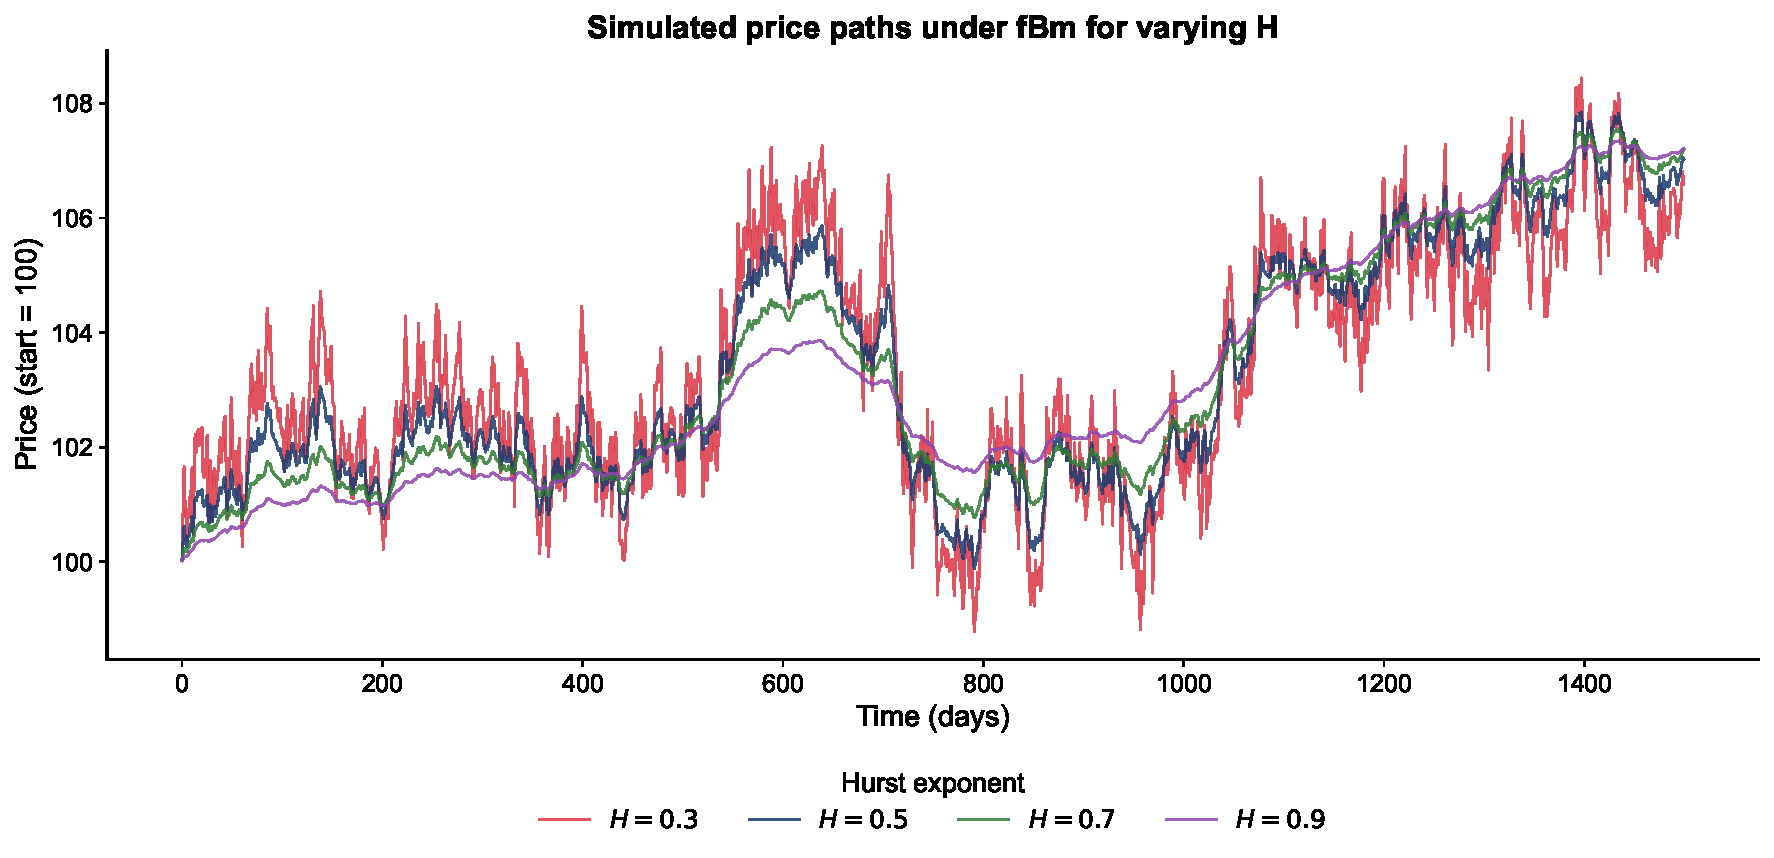
\includegraphics[width=\linewidth,height=4.6cm,keepaspectratio]{ch_fmh_price_paths_H.pdf}\\[2pt]
{\scriptsize\textcolor{MediumGray}{\textit{Traiectorii de preț simulate pentru patru valori ale $H$.}}}
\figql{SFM\_ch\_fmh\_extra: price\_paths\_H}{https://github.com/danpele/SFM/tree/main/Quantlets/SFM_ch_fmh}
\end{column}
\end{columns}
\end{cminipage}
\end{frame}

\slidelevel{Y3}
\begin{frame}[shrink=10]{EMH vs FMH: comparație directă}
\begin{cminipage}{0.95\textwidth}
\begin{columns}[T]
\begin{column}{0.48\textwidth}
\begin{block}{EMH}
\begin{itemize}\setlength{\itemsep}{0pt}
    \item Toți investitorii au \textbf{același orizont}
    \item Informația reflectată \textbf{instantaneu}
    \item Randamente \textbf{i.i.d.} (independent and identically distributed), varianță finită
    \item Mers aleator (Brown), $H=0{,}5$
\end{itemize}
\end{block}
\end{column}
\begin{column}{0.48\textwidth}
\begin{alertblock}{FMH}
\begin{itemize}\setlength{\itemsep}{0pt}
    \item Investitori pe \textbf{orizonturi multiple}
    \item Stabilitatea $\propto$ \textbf{diversitatea orizonturilor}
    \item Randamente cu \textbf{autosimilaritate} și memorie
    \item De obicei $H\neq 0{,}5$ (cel mai des $H>0{,}5$)
\end{itemize}
\end{alertblock}
\end{column}
\end{columns}
\vspace{0.2cm}
\begin{exampleblock}{Idee centrală}
\begin{itemize}\setlength{\itemsep}{0pt}
    \item Traderii pe termen scurt vând $\Rightarrow$ investitorii pe termen lung cumpără $\Rightarrow$ \textbf{lichiditate}
    \item Cu orizonturi omogene, lichiditatea \textbf{dispare}
\end{itemize}
\end{exampleblock}
\end{cminipage}
\end{frame}

\slidelevel{Y3}
\begin{frame}[shrink=10]{Orizonturi multiple și diversitate de orizonturi}
\begin{cminipage}{0.95\textwidth}
\begin{columns}[T]
\begin{column}{0.55\textwidth}
\begin{itemize}\setlength{\itemsep}{1pt}
    \item Cinci cohorte tipice de investitori:
    \begin{itemize}\setlength{\itemsep}{0pt}
        \item HFT: milisecunde--minute
        \item Day traders: ore--zile
        \item Swing/position: săpt.--luni
        \item Hedge funds: luni--ani
        \item Pensii, sovereign: ani--decenii
    \end{itemize}
    \item \textbf{Diversitate de orizonturi} = răspândirea ponderilor pe cohortele de mai sus
    \item \textbf{Colapsul orizonturilor} = ponderile se concentrează pe o singură cohortă (de regulă cea scurtă)
\end{itemize}
\end{column}
\begin{column}{0.42\textwidth}
\begin{exampleblock}{Proxy didactic --- entropia orizonturilor}
\begin{itemize}\setlength{\itemsep}{0pt}
    \item Folosim entropia $\mathcal{H}_{\text{horiz}}=-\sum_i w_i\log w_i$ ca \textbf{proxy didactic} al diversității participanților
    \item \textbf{Nu este o lege formală a FMH}, ci doar o ilustrație
    \item $\mathcal{H}_{\text{horiz}}$ mare $\Leftrightarrow$ orizonturi diverse
\end{itemize}
\end{exampleblock}
\end{column}
\end{columns}
\end{cminipage}
\end{frame}

\slidelevel{Y3}
\begin{frame}[shrink=10]{Crahuri ca colaps al orizonturilor}
\begin{cminipage}{0.95\textwidth}
\begin{block}{Naratorul informal (FMH)}
\begin{itemize}\setlength{\itemsep}{2pt}
    \item Un \textbf{șoc fundamental} (Lehman, COVID) afectează simultan toate orizonturile
    \item Investitorii pe termen lung adoptă comportament pe termen scurt (vânzare în panică)
    \item Distribuția orizonturilor \textbf{colapsează} $\Rightarrow$ \textbf{lichiditatea dispare}
    \item Structura fractală se rupe $\Rightarrow$ $\hat{H}_t$ se schimbă brusc
\end{itemize}
\end{block}
\begin{exampleblock}{Evidență}
\begin{itemize}\setlength{\itemsep}{0pt}
    \item Criza 2008: $\hat{H}_t$ pe S\&P~500 a scăzut spre $0{,}5$ (Dominique \& Rivera, 2011)
    \item COVID martie 2020: colaps al diversității în câteva zile
    \item \textbf{Derivare formală în Anexa~D}
\end{itemize}
\end{exampleblock}
\end{cminipage}
\end{frame}

\slidelevel{Y3}
\begin{frame}{Recap §1: 3 idei-cheie}
\begin{cminipage}{0.95\textwidth}
\begin{block}{De reținut}
\begin{enumerate}\setlength{\itemsep}{4pt}
    \item EMH (Cap.~4) e utilă dar incompletă: nu explică heavy tails, vol. clustering, memorie lungă, crahuri
    \item FMH propune \textbf{piețe fractale + orizonturi multiple}; stabilitatea piețelor depinde de \textbf{diversitatea orizonturilor}
    \item Crahurile = \textbf{colapsul} acestei diversități; semnal observabil: $\hat{H}_t$ scade brusc spre (sau sub) $0{,}5$
\end{enumerate}
\end{block}
\end{cminipage}
\end{frame}

%#############################################################################
\section{Fractali și scalare: intuiția}
%#############################################################################

\slidelevel{Y3}
\begin{frame}{Ce învățăm aici și de ce contează în finanțe?}
\begin{cminipage}{0.95\textwidth}
\begin{block}{Obiectivele §2}
\begin{itemize}\setlength{\itemsep}{2pt}
    \item Definim \textbf{dimensiunea fractală} $D$ pe exemple simple (Koch, Sierpinski)
    \item Înțelegem ,,paradoxul țărmurilor'' și legătura $L(\varepsilon)\propto\varepsilon^{1-D}$
    \item Vedem că graficul \textbf{prețului} are $D=2-H$ --- preț ca fractal statistic
    \item Punte: §1 a dat motivația; aici intrăm în geometrie pentru a măsura ,,cât e neregulat''
\end{itemize}
\end{block}
\end{cminipage}
\end{frame}

\slidelevel{Y3}
\begin{frame}[shrink=15]{Dimensiunea fractală: definiție simplă}
\begin{cminipage}{0.95\textwidth}
\begin{defn}[Dimensiunea de similaritate]
Dacă un obiect autosimilar se descompune în $N$ copii la scara $r=1/s$:
\[
    \boxed{\; D = \frac{\log N}{\log s} = \frac{\log N}{\log(1/r)} \;}
\]
\end{defn}
\begin{columns}[T]
\begin{column}{0.50\textwidth}
\begin{block}{Sanity check (cazuri întregi)}
\begin{itemize}\setlength{\itemsep}{0pt}
    \item Linie: $N=2,\,r=1/2 \Rightarrow D=1$
    \item Pătrat: $N=4,\,r=1/2 \Rightarrow D=2$
    \item Cub: $N=8,\,r=1/2 \Rightarrow D=3$
\end{itemize}
\end{block}
\end{column}
\begin{column}{0.50\textwidth}
\begin{alertblock}{Cazuri fractale}
\begin{itemize}\setlength{\itemsep}{0pt}
    \item Cantor: $D\approx 0{,}631$
    \item Koch: $D\approx 1{,}262$
    \item Sierpinski: $D\approx 1{,}585$
\end{itemize}
\end{alertblock}
\end{column}
\end{columns}
\vspace{0.1cm}
\begin{exampleblock}{Cheie de citire pentru piețe}
\begin{itemize}\setlength{\itemsep}{0pt}
    \item Graficul prețului are $D=2-H$ (Mandelbrot 1968)
    \item $D$ măsoară cât de neregulat este graficul
\end{itemize}
\end{exampleblock}
\end{cminipage}
\end{frame}

\slidelevel{Y3}
\begin{frame}[shrink=10]{Țărmurile fractale: ,,Cât de lungă este coasta Britaniei?''}
\begin{cminipage}{0.96\textwidth}
\begin{itemize}\setlength{\itemsep}{1pt}
    \item \textbf{Construcție}
    \begin{itemize}\setlength{\itemsep}{0pt}
        \item Mandelbrot (1967, \textit{Science}): lungimea măsurată depinde de \textbf{rigla} $\varepsilon$ folosită
        \item Legea de scalare: $L(\varepsilon)\propto\varepsilon^{1-D}$; pentru $D>1$, $L\to\infty$ când $\varepsilon\to 0$
    \end{itemize}
    \item \textbf{Evidență empirică}
    \begin{itemize}\setlength{\itemsep}{0pt}
        \item Britania: $D\approx 1{,}25$; Norvegia: $D\approx 1{,}52$ \quad $\Rightarrow$ \quad ,,riggle--coastline'' problem
        \item \textbf{Analogia financiară}: graficul prețului are $D=2-H$ --- aceeași dependență de scală
    \end{itemize}
\end{itemize}
\centering
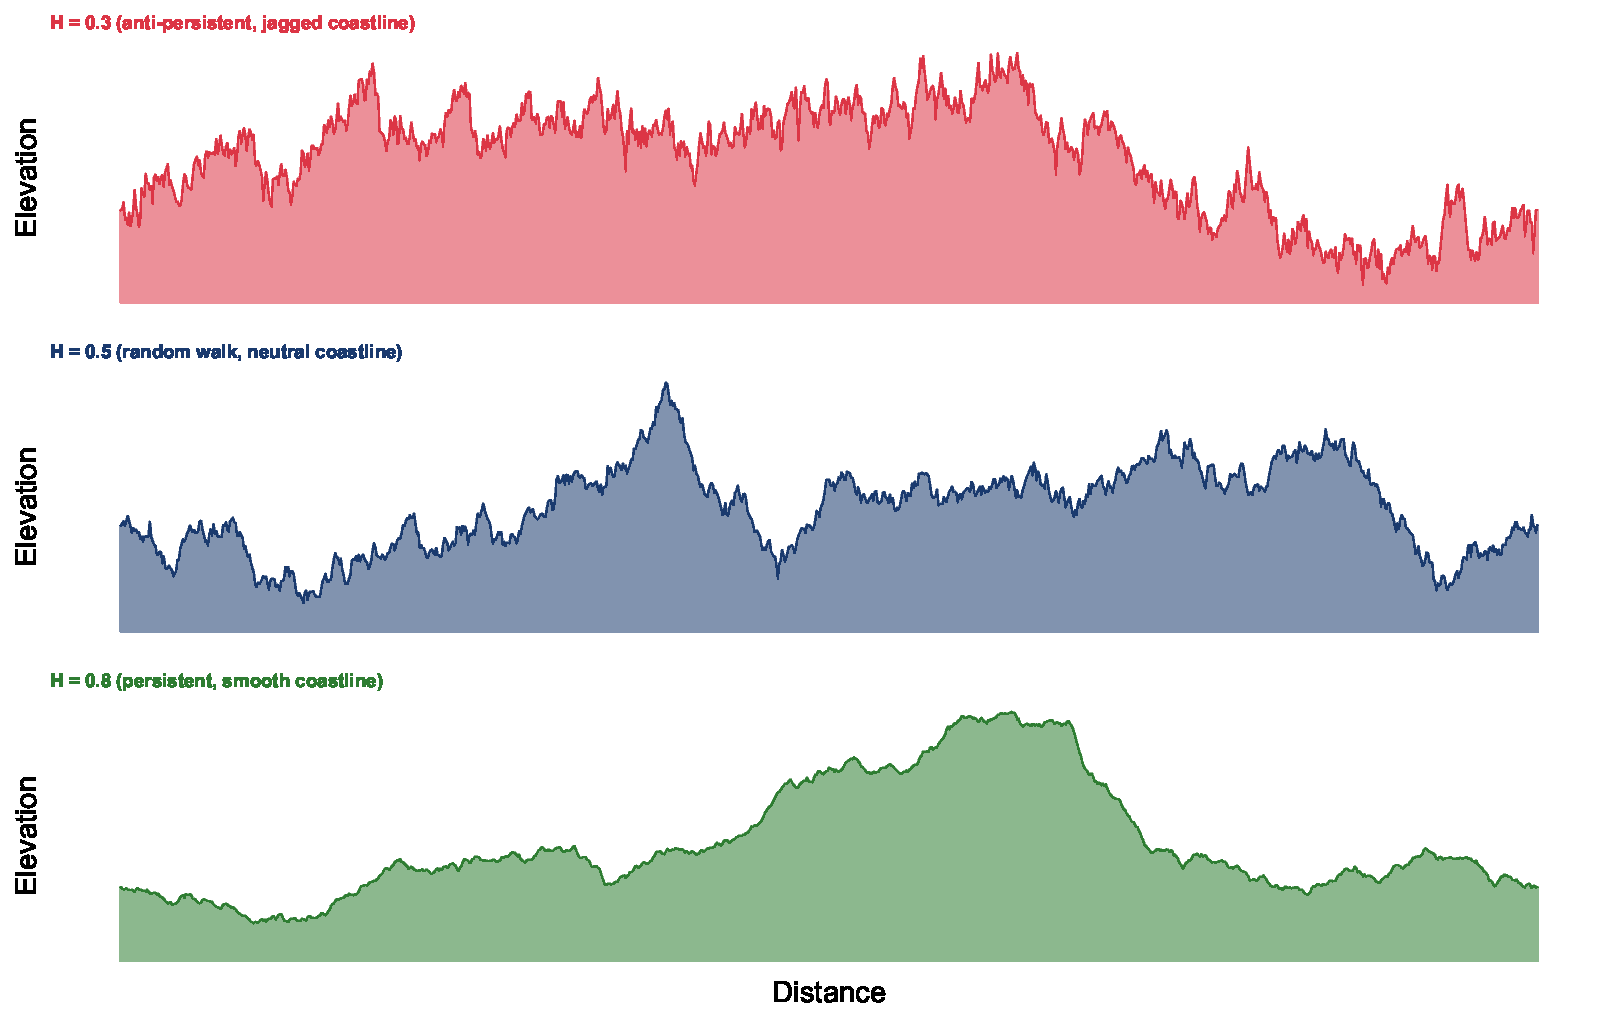
\includegraphics[width=0.95\linewidth,height=3.7cm,keepaspectratio]{ch_fmh_coastline.pdf}\\[1pt]
{\scriptsize\textcolor{MediumGray}{\textit{Țărmul real al Marii Britanii (Natural Earth 1:10m). Box-counting: $N(\varepsilon)$ crește când $\varepsilon$ scade --- pantă $\approx D$.}}}
\figql{SFM\_ch\_fmh\_fractals: coastline}{https://github.com/danpele/SFM/tree/main/Quantlets/SFM_ch_fmh}
\end{cminipage}
\end{frame}

\slidelevel{Y3}
\begin{frame}[shrink=10]{Curba Koch: lungime dependentă de scală}
\begin{cminipage}{0.96\textwidth}
\begin{itemize}\setlength{\itemsep}{1pt}
    \item \textbf{Construcție}
    \begin{itemize}\setlength{\itemsep}{0pt}
        \item Construcție Koch (1904): la fiecare iterație fiecare segment $\to$ 4 segmente de lungime $1/3$
        \item Lungime infinită, arie finită; dimensiune $D=\log 4/\log 3\approx 1{,}262$
    \end{itemize}
    \item \textbf{Interpretare}
    \begin{itemize}\setlength{\itemsep}{0pt}
        \item Prototip pentru \textbf{lungime dependentă de scală} --- aceeași idee ca la țărmul Britaniei
    \end{itemize}
\end{itemize}
\centering
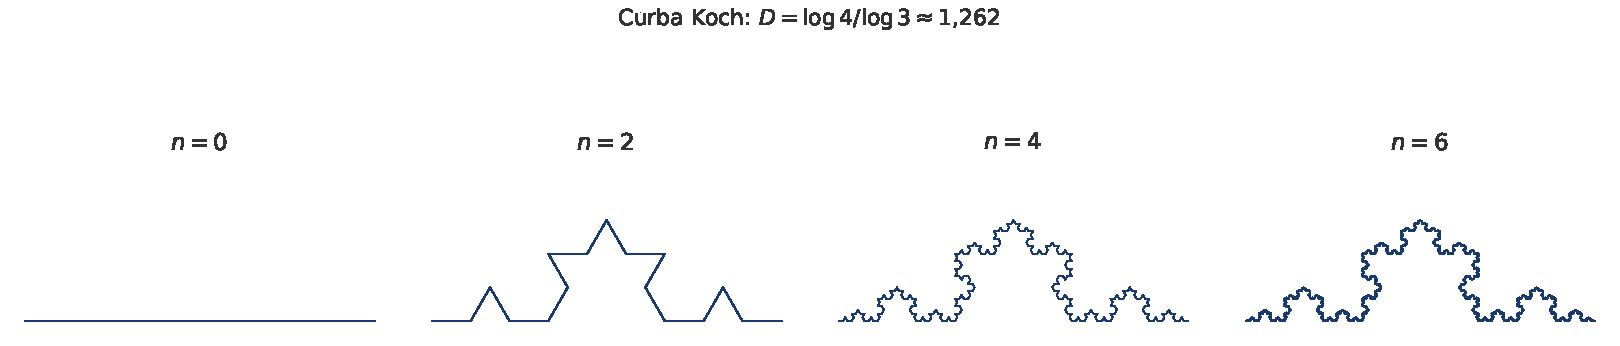
\includegraphics[width=0.95\linewidth,height=3.6cm,keepaspectratio]{ch_fmh_koch_curve.pdf}\\[1pt]
{\scriptsize\textcolor{MediumGray}{\textit{Curba Koch la iterațiile $n=0,2,4,6$ (curba reală, fără simboluri stilizate).}}}
\figql{SFM\_ch\_fmh\_fractals: koch\_curve}{https://github.com/danpele/SFM/tree/main/Quantlets/SFM_ch_fmh}
\end{cminipage}
\end{frame}

\slidelevel{Y3}
\begin{frame}{Triunghiul Sierpinski}
\begin{cminipage}{0.96\textwidth}
\begin{columns}[T]
\begin{column}{0.45\textwidth}
\begin{itemize}\setlength{\itemsep}{2pt}
    \item Construit prin \textit{chaos game} sau eliminare iterativă
    \item $N=3$ copii la $r=1/2$
    \item Dimensiune: $D=\log 3/\log 2\approx 1{,}585$
\end{itemize}
\end{column}
\begin{column}{0.53\textwidth}
\centering
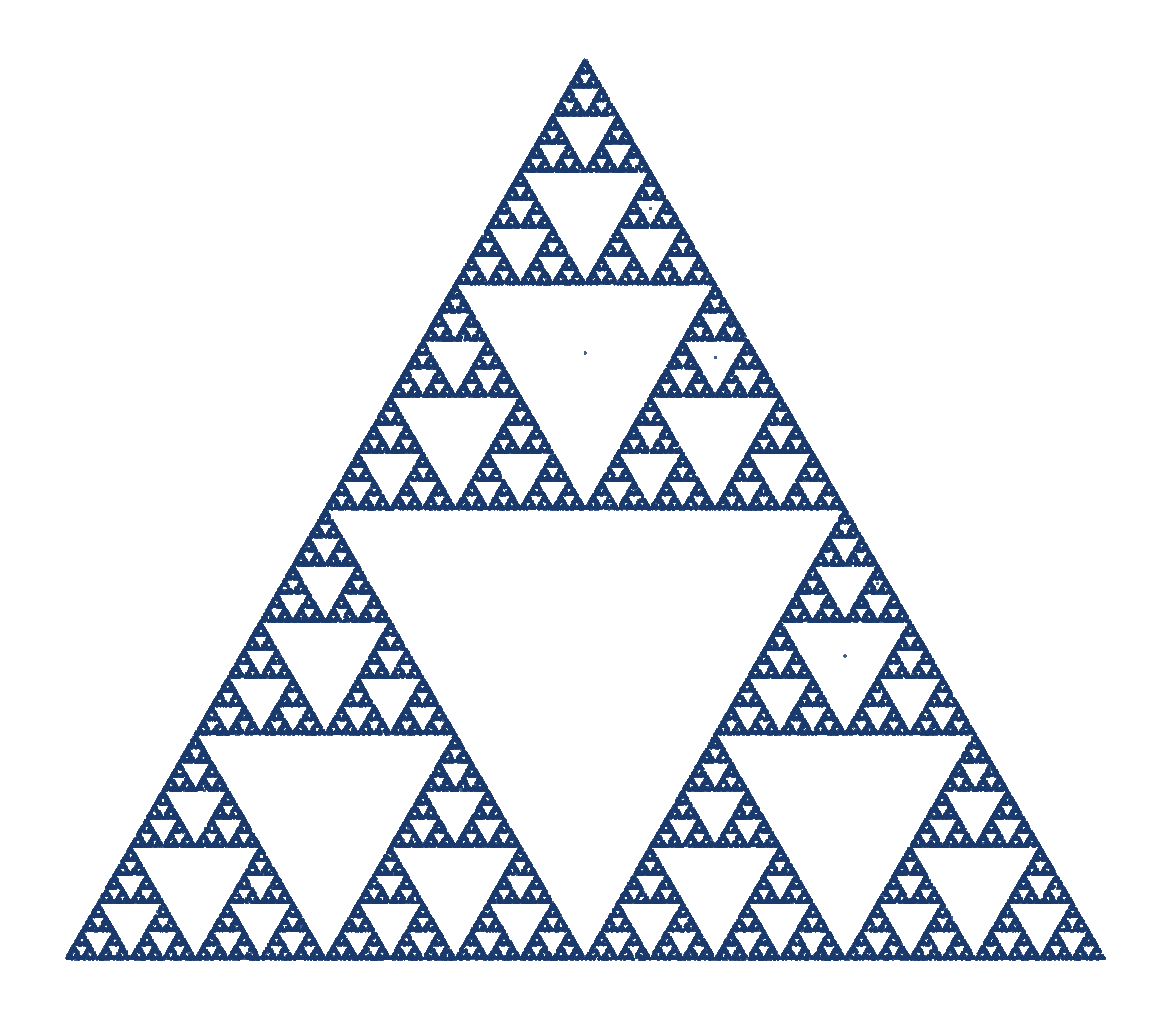
\includegraphics[height=4.6cm,keepaspectratio]{ch_fmh_sierpinski.pdf}
\figql{SFM\_ch\_fmh\_fractals: sierpinski}{https://github.com/danpele/SFM/tree/main/Quantlets/SFM_ch_fmh}
\end{column}
\end{columns}
\end{cminipage}
\end{frame}

\slidelevel{Y3}
\begin{frame}[shrink=10]{Prețul ca fractal}
\begin{cminipage}{0.95\textwidth}
\begin{itemize}\setlength{\itemsep}{0pt}
    \item Mandelbrot (1963, 2004): \textit{,,Markets are turbulent like fluids and fractal like coastlines.''}
    \item Intraday vs daily vs weekly $\Rightarrow$ același tip de variabilitate statistică
\end{itemize}
\centering
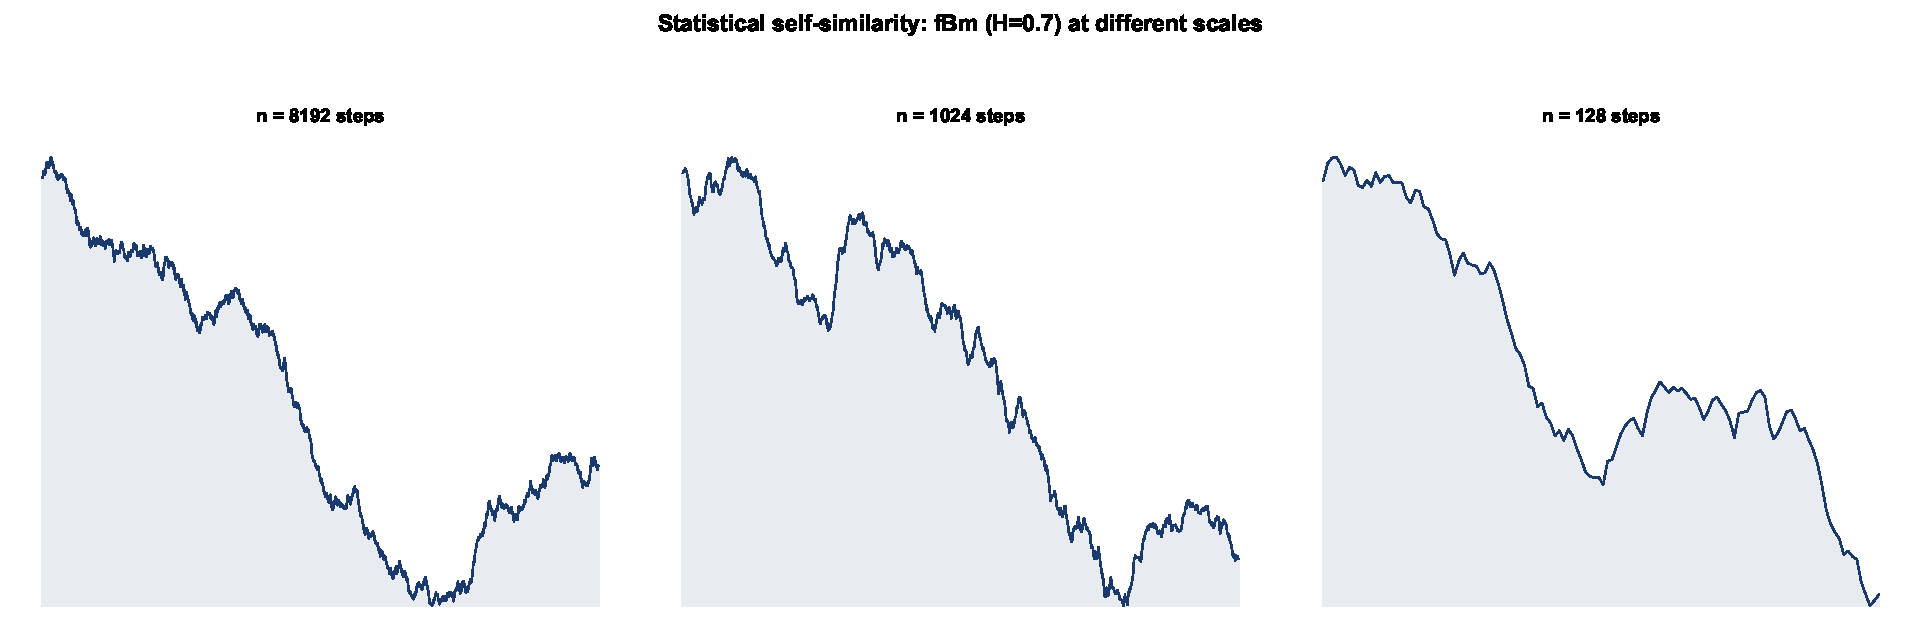
\includegraphics[height=4.6cm,keepaspectratio]{ch_fmh_selfsimilarity.pdf}\\[2pt]
{\scriptsize\textcolor{MediumGray}{\textit{Aceeași traiectorie fBm la trei nivele de zoom --- structura statistică se conservă.}}}
\figql{SFM\_ch\_fmh\_fractals: selfsimilarity}{https://github.com/danpele/SFM/tree/main/Quantlets/SFM_ch_fmh}
\end{cminipage}
\end{frame}

\slidelevel{Y3}
\begin{frame}{Recap §2: 3 idei-cheie}
\begin{cminipage}{0.95\textwidth}
\begin{block}{De reținut}
\begin{enumerate}\setlength{\itemsep}{4pt}
    \item Dimensiunea fractală $D=\log N/\log(1/r)$ măsoară ,,cât de neregulat'' este un obiect autosimilar
    \item ,,Coasta Britaniei'': $L(\varepsilon)\propto\varepsilon^{1-D}$ --- introduce ideea de scalare dependentă de scală
    \item Pentru piețe: graficul prețului are $D=2-H$; prețul este \textbf{fractal statistic}, nu doar mers aleator
\end{enumerate}
\end{block}
\end{cminipage}
\end{frame}

%#############################################################################
\section{Autosimilaritate și dimensiune fractală}
%#############################################################################

\slidelevel{Y3}
\begin{frame}{Ce învățăm aici și de ce contează în finanțe?}
\begin{cminipage}{0.95\textwidth}
\begin{block}{Obiectivele §3}
\begin{itemize}\setlength{\itemsep}{2pt}
    \item Definim \textbf{autosimilaritatea statistică} (proces $H$-autosimilar)
    \item Construim mulțimea Cantor --- primul fractal modern
    \item Introducem \textbf{dimensiunea box-counting} (estimabilă numeric)
    \item Punte: §2 a dat intuiția vizuală; aici trecem la procese stocastice (preț, randament)
\end{itemize}
\end{block}
\end{cminipage}
\end{frame}

\slidelevel{Y3}
\begin{frame}[shrink=10]{Mulțimea Cantor: primul fractal}
\begin{cminipage}{0.96\textwidth}
\begin{columns}[T]
\begin{column}{0.48\textwidth}
\begin{defn}[Mulțimea Cantor]
Pornind de la $C_0=[0,1]$, la fiecare pas se elimină \textbf{treimea de mijloc} a fiecărui interval. $C=\bigcap_{k\geq 0} C_k$.
\end{defn}
\begin{itemize}\setlength{\itemsep}{0pt}
    \item Lungime totală $0$, infinitate nenumărabilă de puncte
    \item Dimensiune: $D=\log 2/\log 3\approx 0{,}631$
\end{itemize}
\end{column}
\begin{column}{0.50\textwidth}
\centering
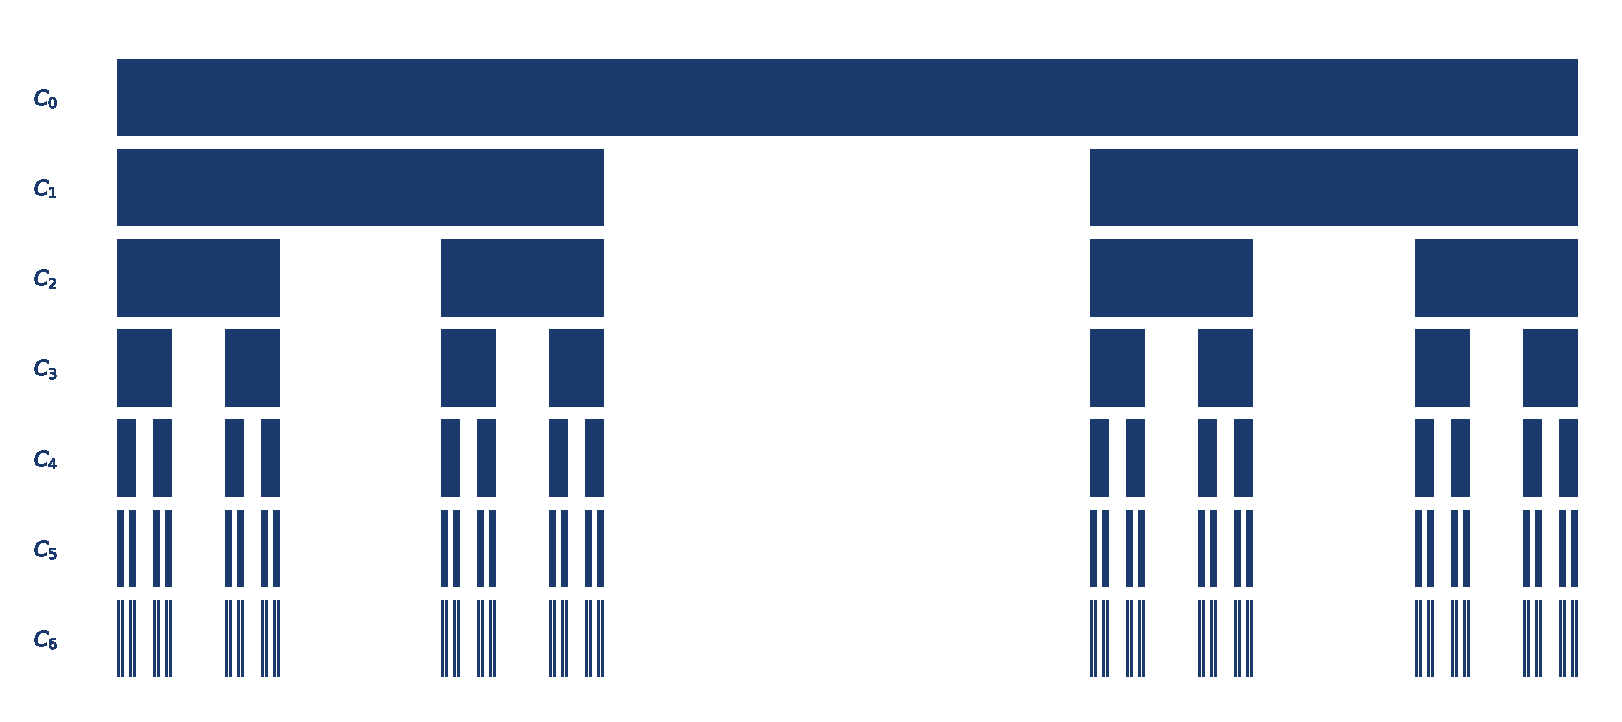
\includegraphics[width=\linewidth]{ch_fmh_cantor.pdf}\\[2pt]
{\scriptsize\textcolor{MediumGray}{\textit{Primele 7 iterații în construcția mulțimii Cantor.}}}
\figql{SFM\_ch\_fmh\_fractals: cantor}{https://github.com/danpele/SFM/tree/main/Quantlets/SFM_ch_fmh}
\end{column}
\end{columns}
\end{cminipage}
\end{frame}

\slidelevel{MSc}
\begin{frame}[shrink=15]{Autosimilaritate exactă vs statistică}
\begin{cminipage}{0.95\textwidth}
\begin{defn}[Proces autosimilar (statistic)]
$\{X(t)\}_{t\geq 0}$ este \textbf{$H$-autosimilar} dacă, pentru orice $c>0$,
\[
    \{X(ct)\}_{t\geq 0}\stackrel{d}{=}\{c^{H} X(t)\}_{t\geq 0}.
\]
\end{defn}
\begin{columns}[T]
\begin{column}{0.50\textwidth}
\begin{block}{Exact (deterministic)}
\begin{itemize}\setlength{\itemsep}{0pt}
    \item $S=\bigcup_{i=1}^N f_i(S)$ cu $f_i$ contracții
    \item Cantor, Koch, Sierpinski, Mandelbrot
\end{itemize}
\end{block}
\end{column}
\begin{column}{0.48\textwidth}
\begin{alertblock}{Statistic (random)}
\begin{itemize}\setlength{\itemsep}{0pt}
    \item Distribuții finit-dim. invariante la scalare $c^H$
    \item fBm, fGn (fractional Gaussian noise), cascade multiplicative
    \item \textbf{Cazul piețelor}: auto-afinitate (timp $\neq$ preț)
\end{itemize}
\end{alertblock}
\end{column}
\end{columns}
\vspace{0.15cm}
\begin{exampleblock}{Legea de scalare a volatilității}
\begin{itemize}\setlength{\itemsep}{0pt}
    \item Dacă $\ln P(t)$ este $H$-autosimilar: $\sigma(\Delta)=\sigma(1)\cdot \Delta^{H}$
    \item Sub EMH ($H=0{,}5$): regula clasică $\sqrt{\Delta}$
\end{itemize}
\end{exampleblock}
\end{cminipage}
\end{frame}

\slidelevel{MSc}
\begin{frame}[shrink=10]{Dimensiunea fractală box-counting}
\begin{cminipage}{0.95\textwidth}
\begin{defn}[Box-counting / Minkowski-Bouligand]
Fie $S\subset\R^d$ mărginită și $N(\varepsilon)$ numărul minim de cuburi de latură $\varepsilon$ care acoperă $S$:
\[
    D_{\text{box}}=\lim_{\varepsilon\to 0^+}\frac{\log N(\varepsilon)}{\log(1/\varepsilon)}.
\]
\end{defn}
\begin{itemize}\setlength{\itemsep}{0pt}
    \item \textbf{Estimare}
    \begin{itemize}\setlength{\itemsep}{0pt}
        \item Estimată empiric prin regresie liniară a $\log N(\varepsilon)$ pe $\log(1/\varepsilon)$
    \end{itemize}
    \item \textbf{Proprietăți}
    \begin{itemize}\setlength{\itemsep}{0pt}
        \item Pentru fractali ,,bine-comportați'': $D_{\text{box}}=\dim_H$ (Hausdorff)
        \item Cea mai folosită numeric --- \textbf{Hausdorff} = standard matematic, dar dificil de calculat (vezi Anexa~D)
    \end{itemize}
\end{itemize}
\end{cminipage}
\end{frame}

\slidelevel{MSc}
\begin{frame}[shrink=10]{Dimensiuni fractale alternative}
\begin{cminipage}{0.95\textwidth}
\begin{itemize}\setlength{\itemsep}{1pt}
    \item Există mai multe variante de dimensiune fractală:
    \begin{itemize}\setlength{\itemsep}{0pt}
        \item Hausdorff $D_H$ --- standard riguros, dificil numeric
        \item Box-counting $D_{\text{box}}$ --- standardul empiric
        \item Similaritate $D_S$ --- pentru IFS (Iterated Function System) auto-similare
        \item Informație $D_I$, corelație $D_C$, $q$-dimensiune $D_q$ --- multifractali
    \end{itemize}
    \item Pentru \textbf{monofractali}: toate dimensiunile coincid, $D_H=D_{\text{box}}=D_q$
    \item Pentru \textbf{multifractali}: $D_q$ depinde de $q$ $\Rightarrow$ \textbf{spectru de dimensiuni} (vezi §6, Anexa~D)
\end{itemize}
\end{cminipage}
\end{frame}

\slidelevel{Y3}
\begin{frame}{Recap §3: 3 idei-cheie}
\begin{cminipage}{0.95\textwidth}
\begin{block}{De reținut}
\begin{enumerate}\setlength{\itemsep}{4pt}
    \item Cantor = primul fractal modern; $D=\log 2/\log 3\approx 0{,}631$
    \item Autosimilaritate statistică: $X(ct)\stackrel{d}{=}c^H X(t)$ --- conduce la $\sigma(\Delta)=\sigma(1)\Delta^H$
    \item Box-counting este standardul empiric; alte variante (Hausdorff etc.) coincid pe monofractali, diverg pe multifractali
\end{enumerate}
\end{block}
\end{cminipage}
\end{frame}

%#############################################################################
\section{Exponentul Hurst}
%#############################################################################

\slidelevel{Y3}
\begin{frame}{Ce învățăm aici și de ce contează în finanțe?}
\begin{cminipage}{0.95\textwidth}
\begin{block}{Obiectivele §4}
\begin{itemize}\setlength{\itemsep}{2pt}
    \item Cum a apărut $H$: Hurst la Nilul (1951), apoi Mandelbrot \& Wallis (1969)
    \item Definiție formală și interpretare a celor 3 regimuri
    \item \textbf{Avertisment}: $H>0{,}5$ NU înseamnă automat profit exploatabil
    \item Punte: §3 a dat scalarea $\sigma(\Delta)=\sigma(1)\Delta^H$; aici facem $H$-ul observabil din date
\end{itemize}
\end{block}
\end{cminipage}
\end{frame}

\slidelevel{Y3}
\begin{frame}[shrink=10]{Harold Hurst și problema Nilului}
\begin{cminipage}{0.95\textwidth}
\begin{columns}[T]
\begin{column}{0.55\textwidth}
\begin{itemize}\setlength{\itemsep}{1pt}
    \item \textbf{Context}
    \begin{itemize}\setlength{\itemsep}{0pt}
        \item Harold E.~Hurst (1880--1978), hidrolog britanic în Egipt
        \item Niveluri anuale ale Nilului (847--1284 d.Hr.)
    \end{itemize}
    \item \textbf{Observație și estimare}
    \begin{itemize}\setlength{\itemsep}{0pt}
        \item Anii umezi tind să se grupeze; idem cei secetoși $\Rightarrow$ \textbf{dependență pe termen lung}
        \item $\E[R(n)/S(n)]\propto n^H$; pentru Nil: $H\approx 0{,}73$
        \item ,,Efectul Joseph'' (Mandelbrot 1968) după ,,7 ani buni urmați de 7 răi''
    \end{itemize}
\end{itemize}
\end{column}
\begin{column}{0.42\textwidth}
\begin{block}{Mandelbrot \& Wallis (1969)}
\begin{itemize}\setlength{\itemsep}{0pt}
    \item Aplică R/S pe finanțe
    \item ,,Hurst este la geometria fractală ce este Bachelier la mersul aleator''
\end{itemize}
\end{block}
\end{column}
\end{columns}
\end{cminipage}
\end{frame}

\slidelevel{Y3}
\begin{frame}[shrink=10]{Definiția exponentului Hurst}
\begin{cminipage}{0.95\textwidth}
\begin{defn}[Exponentul Hurst]
$H\in(0,1)$ caracterizează structura de dependență pe termen lung. Sub R/S:
\[
    \E\!\left[\frac{R(n)}{S(n)}\right]\propto n^H,\quad n\to\infty.
\]
\end{defn}
\begin{itemize}\setlength{\itemsep}{0pt}
    \item $H=0{,}5$: mers aleator (fără memorie); consistent cu EMH
    \item $H>0{,}5$: persistent (trending); autocorelație pozitivă pe termen lung
    \item $H<0{,}5$: anti-persistent (mean-reverting); autocorelație negativă
\end{itemize}
\end{cminipage}
\end{frame}

\slidelevel{Y3}
\begin{frame}[shrink=10]{Interpretarea celor 3 regimuri}
\begin{cminipage}{0.95\textwidth}
\begin{columns}[T]
\begin{column}{0.55\textwidth}
\begin{itemize}\setlength{\itemsep}{1pt}
    \item Relație Hurst--dimensiune fractală: $\boxed{D=2-H}$
    \item Scalarea volatilității: $\sigma(\Delta)=\sigma(1)\Delta^H$
    \item Autocorelație increment: $\rho(k)\sim k^{2H-2}$
    \item Implicații risc: VaR (Value-at-Risk) scalează cu $T^H$, nu $\sqrt T$
\end{itemize}
\end{column}
\begin{column}{0.42\textwidth}
\renewcommand{\arraystretch}{1.2}
\centering
\begin{tabular}{ccl}
\toprule
$H$ & $D$ & \textbf{Interpretare} \\
\midrule
$0{,}1$ & $1{,}9$ & Foarte anti-persistent \\
$0{,}3$ & $1{,}7$ & Mean-reverting \\
$0{,}5$ & $1{,}5$ & Mers aleator \\
$0{,}7$ & $1{,}3$ & Persistent moderat \\
$0{,}9$ & $1{,}1$ & Foarte persistent \\
\bottomrule
\end{tabular}
\end{column}
\end{columns}
\end{cminipage}
\end{frame}

\slidelevel{Y3}
\begin{frame}{Atenție: interpretarea greșită a lui $H$}
\begin{cminipage}{0.95\textwidth}
\begin{alertblock}{$H>0{,}5$ NU înseamnă profit garantat}
\begin{itemize}\setlength{\itemsep}{2pt}
    \item Persistența nu este sinonimă cu \textbf{ineficiență exploatabilă}
    \item \textbf{Costuri tranzacționale} pot anula avantajul statistic
    \item $\hat{H}$ este \textbf{instabil} pe sub-eșantioane (regimuri, structural breaks)
    \item Test primar pentru ineficiență: \textbf{Hurst/DFA/MFDFA (Multifractal Detrended Fluctuation Analysis) + stabilitate pe regimuri} (rolling windows, Bai--Perron)
\end{itemize}
\end{alertblock}
\begin{exampleblock}{Recomandare}
\begin{itemize}\setlength{\itemsep}{0pt}
    \item Înainte de a interpreta $\hat{H}>0{,}5$ ca semnal de ineficiență, raportează:
    \begin{itemize}\setlength{\itemsep}{0pt}
        \item (i) IC pentru $\hat{H}$; (ii) $\hat{H}$ pe sub-perioade
        \item (iii) test de breakpoint; (iv) backtest cu costuri
    \end{itemize}
\end{itemize}
\end{exampleblock}
\end{cminipage}
\end{frame}

\slidelevel{Y3}
\begin{frame}[shrink=10]{Efectul Joseph și efectul Noah}
\begin{cminipage}{0.95\textwidth}
\begin{columns}[T]
\begin{column}{0.50\textwidth}
\begin{block}{Joseph (memorie lungă)}
\begin{itemize}\setlength{\itemsep}{0pt}
    \item ,,7 ani buni urmați de 7 răi''
    \item Persistență, $H>0{,}5$
    \item Modelat de fBm și ARFIMA (AutoRegressive Fractionally Integrated Moving Average)
\end{itemize}
\end{block}
\end{column}
\begin{column}{0.46\textwidth}
\begin{alertblock}{Noah (cozi grele)}
\begin{itemize}\setlength{\itemsep}{0pt}
    \item Potopul biblic --- evenimente catastrofale, discontinue
    \item Capturat de exponentul $\alpha$ Lévy ($\alpha<2$)
    \item Modelat de procese Lévy stabile (Cap.~2)
\end{itemize}
\end{alertblock}
\end{column}
\end{columns}
\vspace{0.2cm}
\begin{exampleblock}{Combinare}
\begin{itemize}\setlength{\itemsep}{0pt}
    \item Linear fractional stable motion (LFSM): permite simultan memorie lungă (Joseph) și salturi (Noah)
    \item Generalizare a fBm
\end{itemize}
\end{exampleblock}
\end{cminipage}
\end{frame}

\slidelevel{Y3}
\begin{frame}{Hurst --- proprietăți de bază}
\begin{cminipage}{0.95\textwidth}
\begin{itemize}\setlength{\itemsep}{2pt}
    \item \textbf{Notație}
    \begin{itemize}\setlength{\itemsep}{0pt}
        \item Domeniu: $H\in(0,1)$ pentru fBm
        \item Dimensiunea graficului: $D=2-H$
    \end{itemize}
    \item \textbf{Proprietăți statistice}
    \begin{itemize}\setlength{\itemsep}{0pt}
        \item Varianța increment fBm: $\E[(B_H(t+\tau)-B_H(t))^2]=\tau^{2H}$
        \item Autocorelația incrementelor (fGn) pe termen lung: $\rho(k)\sim H(2H-1)k^{2H-2}$
    \end{itemize}
\end{itemize}
\end{cminipage}
\end{frame}

\slidelevel{MSc}
\begin{frame}{Hurst --- extensii și conexiuni}
\begin{cminipage}{0.95\textwidth}
\begin{itemize}\setlength{\itemsep}{2pt}
    \item \textbf{Reprezentare spectrală}
    \begin{itemize}\setlength{\itemsep}{0pt}
        \item Densitatea spectrală: $S(\omega)\sim|\omega|^{1-2H}$ pentru $\omega\to 0$
    \end{itemize}
    \item \textbf{Conexiuni cu alte modele}
    \begin{itemize}\setlength{\itemsep}{0pt}
        \item Conexiunea cu ARFIMA: $d=H-1/2 \in (-1/2,\,1/2)$
        \item Conexiunea cu DFA: exponent $\alpha=H$ pentru fBm/fGn integrat
    \end{itemize}
    \item \textbf{Proprietăți estimator}
    \begin{itemize}\setlength{\itemsep}{0pt}
        \item Robustețe: $\hat{H}$ robust la transformări monotone și zgomot aditiv mic
    \end{itemize}
\end{itemize}
\end{cminipage}
\end{frame}

\slidelevel{Y3}
\begin{frame}{Recap §4: 3 idei-cheie}
\begin{cminipage}{0.95\textwidth}
\begin{block}{De reținut}
\begin{enumerate}\setlength{\itemsep}{4pt}
    \item $H\in(0,1)$ caracterizează memoria; $H=0{,}5$ = EMH/mers aleator; $H>0{,}5$ persistent; $H<0{,}5$ mean-reverting; $D=2-H$
    \item Joseph (memorie lungă) + Noah (cozi grele) sunt cei doi piloni complementari
    \item $\hat{H}>0{,}5$ NU implică automat ineficiență exploatabilă; raportează stabilitate, IC, costuri
\end{enumerate}
\end{block}
\end{cminipage}
\end{frame}

%#############################################################################
\section{Estimarea lui H: R/S și DFA}
%#############################################################################

\slidelevel{MSc}
\begin{frame}{Ce învățăm aici și de ce contează în finanțe?}
\begin{cminipage}{0.95\textwidth}
\begin{block}{Obiectivele §5}
\begin{itemize}\setlength{\itemsep}{2pt}
    \item Cum se calculează \textbf{operațional} $\hat{H}$: R/S clasic și DFA
    \item Lo (1991) modified R/S --- corecție pentru \textbf{short-range dependence}
    \item Limitările R/S/DFA și combo recomandat
    \item Aplicație directă pe SPY, BTC, EUR/USD
\end{itemize}
\end{block}
\end{cminipage}
\end{frame}

\slidelevel{MSc}
\begin{frame}[shrink=10]{R/S --- pași simpli (pseudocod)}
\begin{cminipage}{0.95\textwidth}
\begin{block}{Algoritm R/S pentru o serie $\{x_1,\ldots,x_N\}$}
\begin{enumerate}\setlength{\itemsep}{1pt}
    \item Pentru $n\in\{n_1,\ldots,n_K\}$ (mărimi de bloc), repetă:
    \begin{itemize}\setlength{\itemsep}{0pt}
        \item Împarte seria în blocuri non-suprapuse de mărime $n$
        \item Pentru fiecare bloc: $Y_k=\sum_{i=1}^k(x_i-\bar{x})$, $R=\max Y_k-\min Y_k$, $S=$ deviația standard
        \item $(R/S)_n=$ media pe blocuri a $R/S$
    \end{itemize}
    \item Regresie OLS: $\log(R/S)_n=\hat{H}\cdot\log n+c$
\end{enumerate}
\end{block}
\begin{exampleblock}{Cod complet în Anexa~C}
\begin{itemize}\setlength{\itemsep}{0pt}
    \item Aici doar pseudocodul
    \item Implementarea Python completă în \textbf{Anexa~C}
\end{itemize}
\end{exampleblock}
\quantlet{SFM\_ch14\_fractal\_hurst}{https://github.com/danpele/SFM/tree/main/Quantlets/SFM_ch14}
\end{cminipage}
\end{frame}

\slidelevel{MSc}
\begin{frame}[shrink=15]{R/S --- exemplu pas-cu-pas pe serie scurtă}
\begin{cminipage}{0.95\textwidth}
\begin{exampleblock}{Date}
\begin{itemize}\setlength{\itemsep}{0pt}
    \item Serie de 8 randamente: $\{0{,}5;\,-0{,}3;\,0{,}8;\,-0{,}2;\,0{,}6;\,-0{,}1;\,0{,}4;\,-0{,}7\}$
    \item Mărime bloc: $n=8$
\end{itemize}
\end{exampleblock}
\begin{itemize}\setlength{\itemsep}{0pt}
    \item Media: $\bar{x}=0{,}125$
    \item Cumulate $Y_k$: $\{0{,}375;\,-0{,}050;\,0{,}625;\,0{,}300;\,0{,}775;\,0{,}550;\,0{,}825;\,0\}$
    \item $R=\max Y-\min Y=0{,}875$; \quad $S=0{,}490$
    \item $R/S=1{,}786$ pentru $n=8$
    \item Repetă pentru $n=4,8,16,\ldots$ și fă regresie OLS
\end{itemize}
\end{cminipage}
\end{frame}

\slidelevel{PhD}
\begin{frame}[shrink=10]{R/S modificată Lo (1991): corecție short-range dependence}
\begin{cminipage}{0.95\textwidth}
\begin{alertblock}{Critica Lo (1991)}
\begin{itemize}\setlength{\itemsep}{0pt}
    \item R/S clasică \textbf{confundă memoria pe termen lung cu memoria pe termen scurt} (autocorelații pe lag-uri mici)
    \item Lo propune o \textbf{corecție pentru short-range dependence}
    \item Corecția vizează autocorelația pe termen scurt, NU GARCH (Generalized AutoRegressive Conditional Heteroskedasticity)
\end{itemize}
\end{alertblock}
\begin{block}{Statistica modificată}
\[
    Q_n=\frac{R(n)}{\sigma_n(q)},\quad
    \sigma_n^2(q)=\hat{\gamma}_0+2\sum_{j=1}^{q}w_j(q)\hat{\gamma}_j,\quad w_j=1-\tfrac{j}{q+1}
\]
cu $\hat{\gamma}_j$ autocovarianța la lag $j$ și $w_j$ ponderi Bartlett (Newey--West).
\end{block}
\begin{itemize}\setlength{\itemsep}{0pt}
    \item Sub $H_0:H=1/2$: $Q_n/\sqrt n \xrightarrow{d} V$ (Lo 1991, Tabel I)
    \item Test la $\alpha=5\%$: respinge dacă $Q_n/\sqrt n\notin[0{,}809,\,1{,}862]$
\end{itemize}
\end{cminipage}
\end{frame}

\slidelevel{MSc}
\begin{frame}[shrink=10]{DFA --- alternativă robustă la trenduri}
\begin{cminipage}{0.95\textwidth}
\begin{block}{Algoritm DFA (Peng et al., 1994)}
\begin{enumerate}\setlength{\itemsep}{1pt}
    \item Calculează profilul $Y_k=\sum_{i=1}^k(x_i-\bar{x})$
    \item Împarte $\{Y_k\}$ în segmente non-suprapuse de mărime $n$
    \item În fiecare segment, ajustează polinom de ordin $m$ (DFA-$m$)
    \item Funcția de fluctuație: $F(n)=\sqrt{\frac{1}{N}\sum(Y_k-\hat{Y}_k^{(m)})^2}$
    \item Regresie: $\log F(n)\sim H\log n$
\end{enumerate}
\end{block}
\begin{itemize}\setlength{\itemsep}{0pt}
    \item Avantaj față de R/S: \textbf{robust la trenduri polinomiale} de grad $\leq m$
    \item Standard: DFA-1 pentru randamente; DFA-2/3 pentru prețuri non-staționare
\end{itemize}
\end{cminipage}
\end{frame}

\slidelevel{PhD}
\begin{frame}{DFA-1, DFA-2, DFA-3: ordinul detrendării}
\begin{cminipage}{0.95\textwidth}
\begin{itemize}\setlength{\itemsep}{2pt}
    \item \textbf{Construcție}
    \begin{itemize}\setlength{\itemsep}{0pt}
        \item DFA-$m$ elimină trenduri polinomiale de grad $\leq m$
        \item Exponent valid în $\alpha\in(0,m+1)$
    \end{itemize}
    \item \textbf{Diagnostic și recomandare}
    \begin{itemize}\setlength{\itemsep}{0pt}
        \item Crossover: $F(n)\sim n^{\alpha_1}$ pentru $n<n^*$, $\sim n^{\alpha_2}$ pentru $n>n^*$ $\Rightarrow$ regimuri multiple
        \item Pentru randamente bursiere: \textbf{DFA-1} sau \textbf{DFA-2}
    \end{itemize}
\end{itemize}
\end{cminipage}
\end{frame}

\slidelevel{MSc}
\begin{frame}[shrink=10]{Comparație metode: R/S, Lo R/S, DFA, MFDFA, GPH, Whittle, wavelet}
\begin{cminipage}{0.95\textwidth}
\renewcommand{\arraystretch}{1.2}
\centering
\small
\begin{tabular}{llll}
\toprule
\textbf{Metodă} & \textbf{Robust trenduri?} & \textbf{Multifractal?} & \textbf{Recomandare} \\
\midrule
R/S clasic (Hurst 1951) & Nu & Nu & Educațional \\
R/S modificat (Lo 1991) & Parțial & Nu & Test formal $H=0{,}5$ \\
DFA-1 (Peng 1994) & Da (linear) & Nu & \textbf{Standard} pentru randamente \\
DFA-2/3 & Da (polinom.) & Nu & Pentru prețuri non-staționare \\
MFDFA (Kantelhardt 2002) & Da & Da & Spectru $h(q),\,f(\alpha)$ \\
GPH (Geweke--Porter-Hudak, 1983) & Nu & Nu & Periodogramă, semi-param \\
Whittle & Da & Nu & Cel mai eficient asimptotic \\
Wavelet (WTMM, Wavelet Transform Modulus Maxima) & Da & Da & Cea mai bună acuratețe \\
\bottomrule
\end{tabular}
\vspace{0.15cm}
\begin{exampleblock}{Combo recomandat}
\begin{itemize}\setlength{\itemsep}{0pt}
    \item DFA-1 (principal) + Variance Ratio (test formal $H=0{,}5$)
    \item R/S Lo (robustețe) + MFDFA (multifractal, dacă există putere de calcul)
\end{itemize}
\end{exampleblock}
\end{cminipage}
\end{frame}

\slidelevel{MSc}
\begin{frame}{Limitări R/S și DFA}
\begin{cminipage}{0.95\textwidth}
\begin{alertblock}{Capcane practice}
\begin{itemize}\setlength{\itemsep}{2pt}
    \item Eșantioane scurte $\Rightarrow$ $\hat{H}$ instabil; IC larg
    \item \textbf{\textit{Structural breaks}} și \textbf{\textit{regime shifts}} pot da $\hat{H}>0{,}5$ \textit{spurious} (Granger \& Ding 1996; Diebold \& Inoue 2001; Mikosch \& Stărică 2004)
    \item \textbf{GARCH} și volatility clustering pot încurca R/S clasic
    \item \textbf{Microstructure noise} la frecvențe înalte
    \item \textbf{Trenduri} non-staționare $\Rightarrow$ folosește DFA-2/3
    \item Alegerea ferestrei $[n_{\min},n_{\max}]$ afectează panta
\end{itemize}
\end{alertblock}
\begin{exampleblock}{Diagnostic}
\begin{itemize}\setlength{\itemsep}{0pt}
    \item Întotdeauna raportează:
    \begin{itemize}\setlength{\itemsep}{0pt}
        \item (a) $\hat{H}$ pe sub-eșantioane (rolling); (b) Bai--Perron breakpoint
        \item (c) DFA pe reziduuri post-detrending
    \end{itemize}
\end{itemize}
\end{exampleblock}
\end{cminipage}
\end{frame}

\slidelevel{MSc}
\begin{frame}[shrink=15]{Aplicație R/S și DFA pe SPY, BTC, EUR/USD}
\begin{cminipage}{0.96\textwidth}
\centering
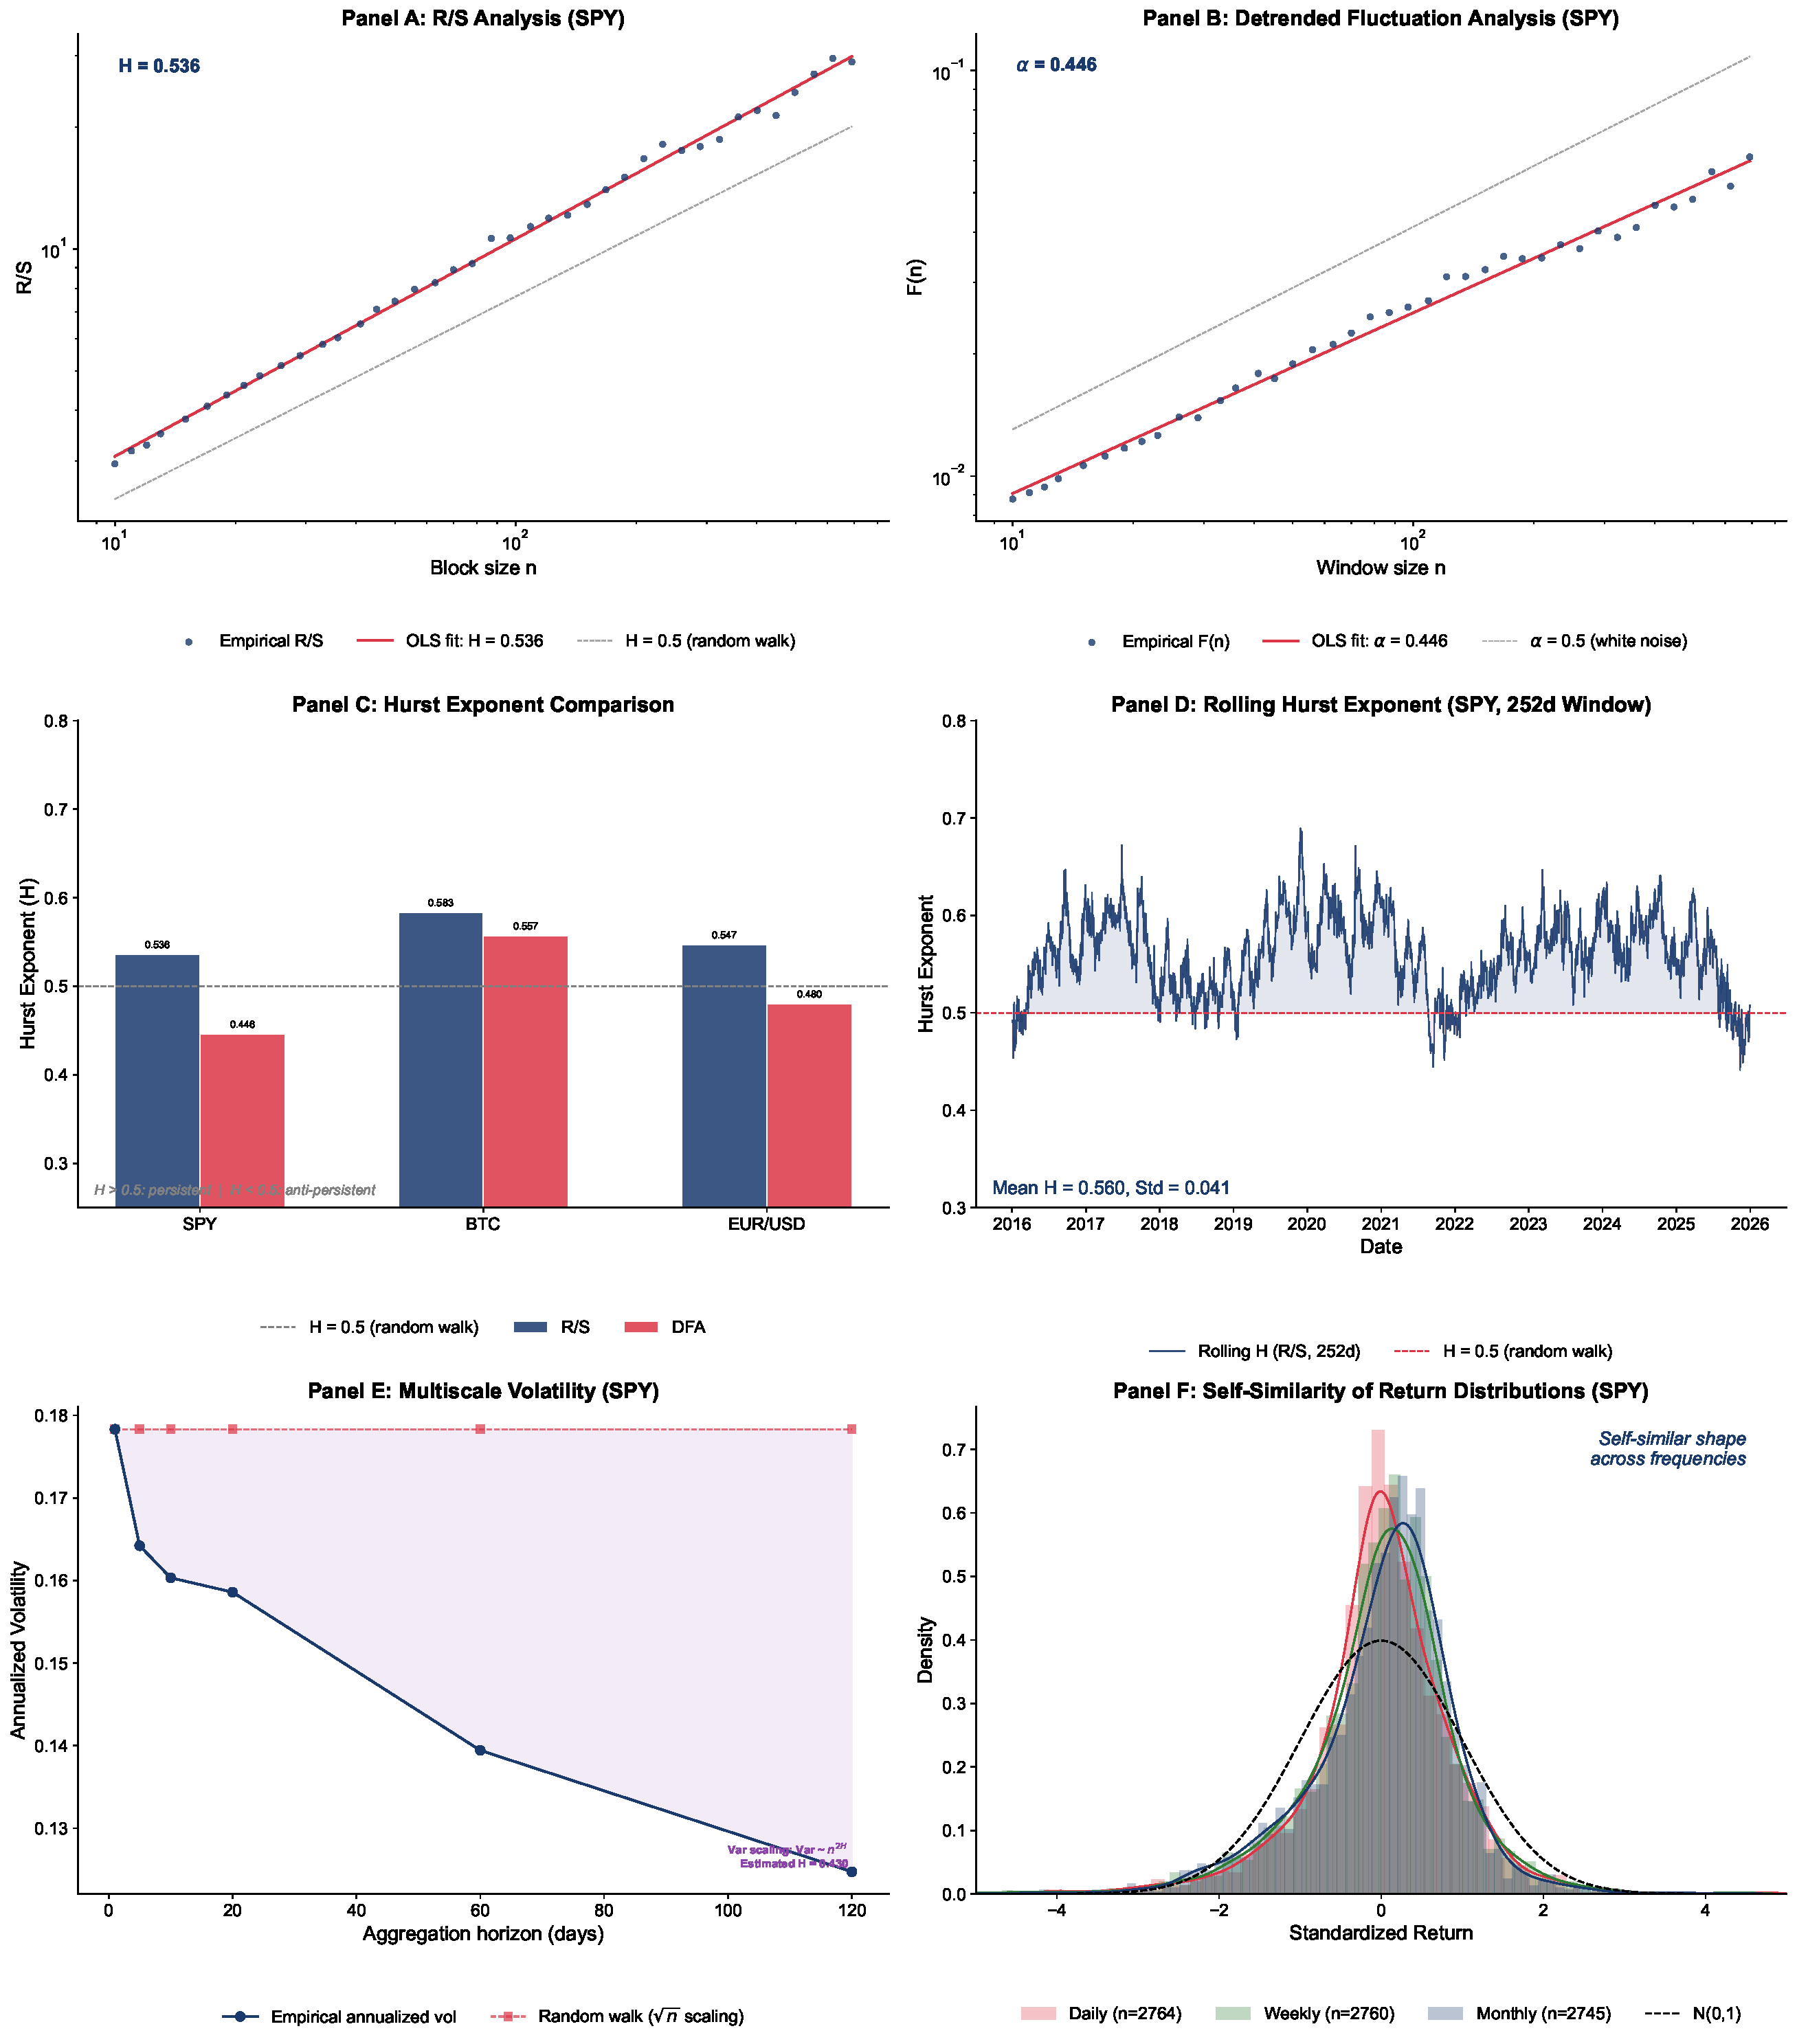
\includegraphics[height=5.4cm]{ch14_fractal_hurst.pdf}\\[2pt]
{\scriptsize\textcolor{MediumGray}{\textit{Panel A: scalarea R/S pe SPY (slope $\approx H$). B: DFA. C: comparație $H$ pe active. D: Hurst rolling. E: scalare volatilitate multi-orizont. F: autosimilaritate distribuțională.}}}
\end{cminipage}
\quantlet{SFM\_ch14\_fractal\_hurst}{https://github.com/danpele/SFM/tree/main/Quantlets/SFM_ch14}
\end{frame}

\slidelevel{Y3}
\begin{frame}{Recap §5: 3 idei-cheie}
\begin{cminipage}{0.95\textwidth}
\begin{block}{De reținut}
\begin{enumerate}\setlength{\itemsep}{4pt}
    \item R/S clasic: pași simpli, dar sensibil la short-range dependence; \textbf{Lo (1991)} corectează cu Newey--West
    \item DFA = standard modern (robust la trenduri polinomiale); MFDFA pentru spectrul multifractal
    \item \textbf{Combo recomandat}: DFA-1 + Variance Ratio + Lo R/S + (opțional) MFDFA; raportează limitări
\end{enumerate}
\end{block}
\end{cminipage}
\end{frame}

%#############################################################################
\section{fBm și multifractalitate}
%#############################################################################

\slidelevel{MSc}
\begin{frame}{Ce învățăm aici și de ce contează în finanțe?}
\begin{cminipage}{0.95\textwidth}
\begin{block}{Obiectivele §6}
\begin{itemize}\setlength{\itemsep}{2pt}
    \item Definiția formală a \textbf{fBm} (folosită informal în §1, §3, §4)
    \item Conexiune fBm $\leftrightarrow$ ARFIMA prin $d=H-1/2$
    \item De la mono- la \textbf{multifractalitate}; MMAR ca generalizare
    \item Punte: §5 ne-a dat $\hat{H}$; aici învățăm modelul stocastic generator
\end{itemize}
\end{block}
\end{cminipage}
\end{frame}

\slidelevel{MSc}
\begin{frame}[shrink=15]{Mișcarea browniană standard (Wiener, 1923)}
\begin{cminipage}{0.95\textwidth}
\begin{defn}[Mișcarea browniană standard]
$\{B(t)\}_{t\geq 0}$ este procesul stocastic cu:
\begin{itemize}\setlength{\itemsep}{0pt}
    \item[(i)] $B(0)=0$
    \item[(ii)] incremenți \textbf{independenți}: $B(t)-B(s)\perp\!\!\!\perp B(u)-B(v)$ pentru intervale disjuncte
    \item[(iii)] incremenți \textbf{gaussieni}: $B(t)-B(s)\sim\mathcal{N}(0,\,t-s)$ pentru $0\leq s<t$
    \item[(iv)] traiectorii \textbf{continue} a.s.
\end{itemize}
\end{defn}
\vspace{0.1cm}
\begin{columns}[T]
\begin{column}{0.50\textwidth}
\begin{block}{Proprietăți care contează aici}
\begin{itemize}\setlength{\itemsep}{0pt}
    \item \textbf{Autosimilaritate} cu $H=1/2$: $B(ct)\stackrel{d}{=}c^{1/2}B(t)$
    \item \textbf{Scalarea volatilității}: $\sigma(\Delta)=\sigma(1)\,\Delta^{1/2}$ (regula $\sqrt{T}$)
    \item Incremenții sunt i.i.d. $\Rightarrow$ \textbf{fără memorie}; ACF $=0$ la orice lag $>0$
    \item Traiectorii continue, dar \textbf{nediferențiabile} a.s.
\end{itemize}
\end{block}
\end{column}
\begin{column}{0.46\textwidth}
\begin{exampleblock}{De ce ne interesează}
\begin{itemize}\setlength{\itemsep}{0pt}
    \item Bachelier (1900): primul model RW al prețurilor folosește $B(t)$
    \item Black--Scholes--Merton (1973): $dS_t=\mu S_t\,dt+\sigma S_t\,dB_t$
    \item Cazul $H=1/2$ al fBm; corespunde EMH în formă slabă
    \item \textbf{Limita}: nu permite memorie sau scalare anormală
\end{itemize}
\end{exampleblock}
\end{column}
\end{columns}
\end{cminipage}
\end{frame}

\slidelevel{MSc}
\begin{frame}[shrink=25]{fBm: definiția formală (Mandelbrot--Van Ness 1968)}
\begin{cminipage}{0.95\textwidth}
\begin{defn}[Mișcarea browniană fracționară]
$\{B_H(t)\}_{t\in\R}$ cu $H\in(0,1)$ este unicul proces gaussian centrat cu $B_H(0)=0$ și covarianța
\[
    \E[B_H(t)B_H(s)]=\tfrac{1}{2}\bigl(|t|^{2H}+|s|^{2H}-|t-s|^{2H}\bigr).
\]
\end{defn}
\begin{columns}[T]
\begin{column}{0.50\textwidth}
\begin{itemize}\setlength{\itemsep}{0pt}
    \item Autosimilaritate: $B_H(ct)\stackrel{d}{=}c^H B_H(t)$
    \item Incremenți staționari, varianță $|t-s|^{2H}$
    \item $H=0{,}5$: mișcare browniană standard
    \item $H>0{,}5$: persistent; $H<0{,}5$: anti-persistent
\end{itemize}
\end{column}
\begin{column}{0.46\textwidth}
\centering
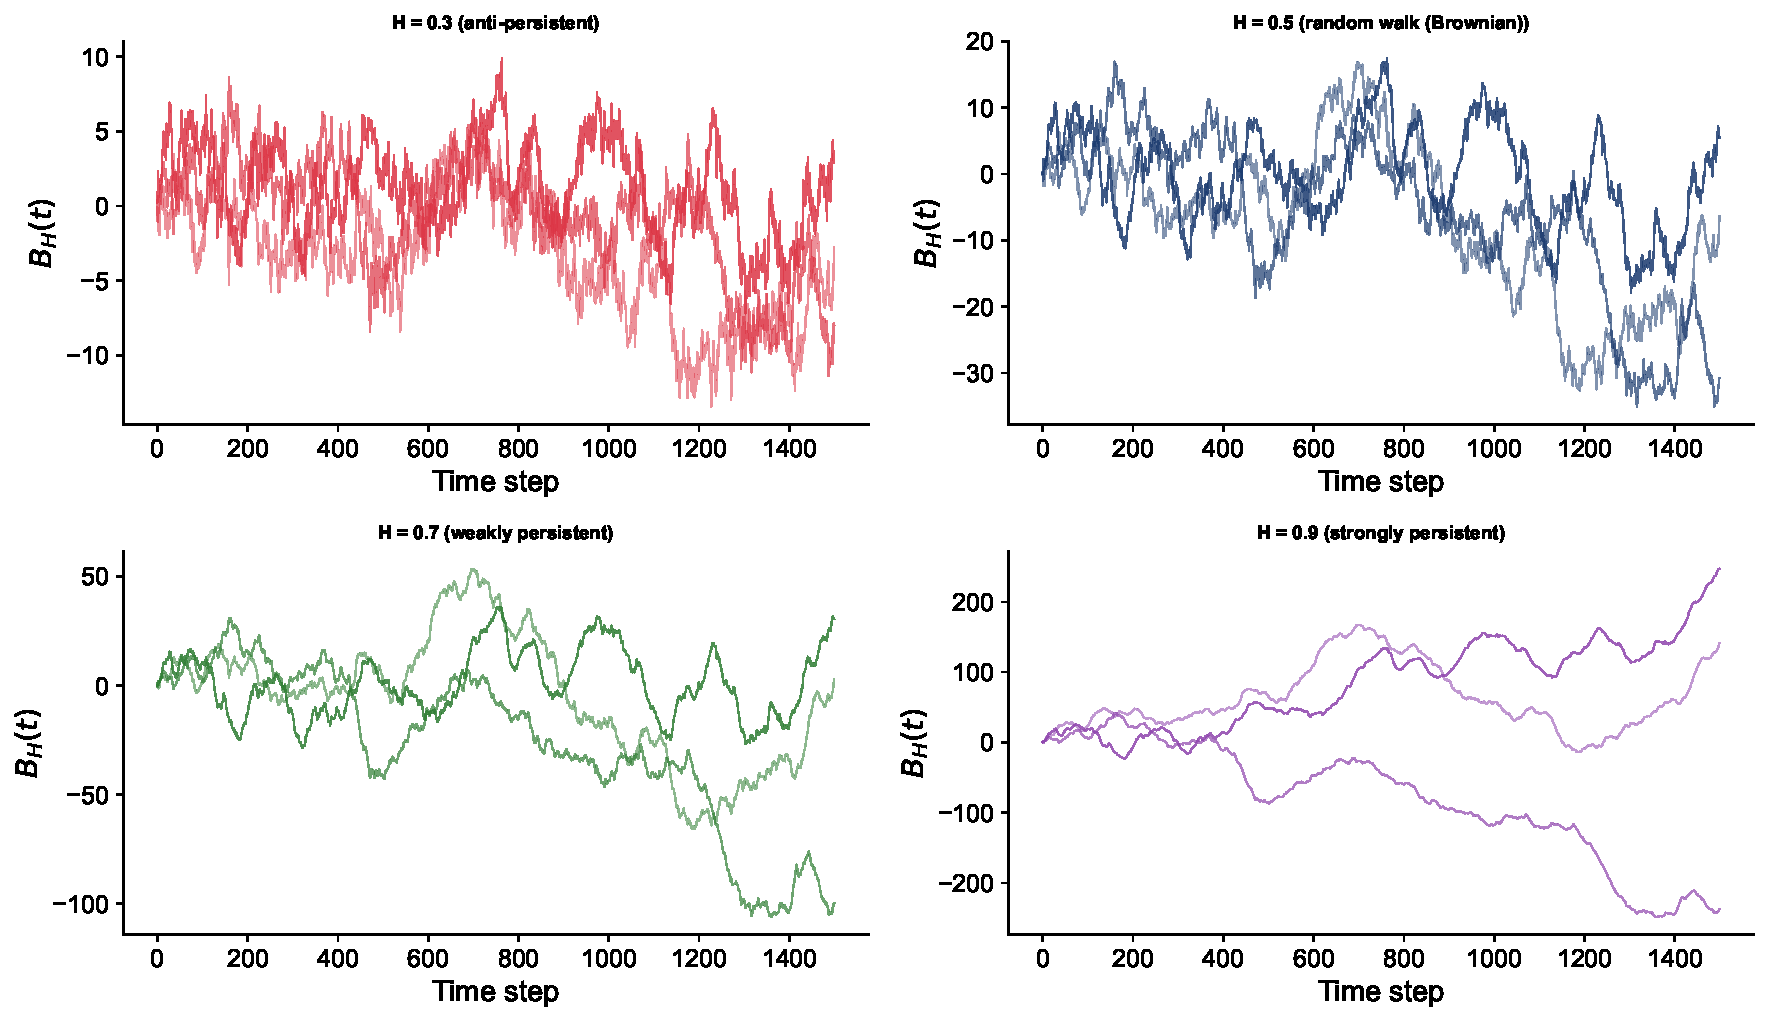
\includegraphics[height=3.6cm,keepaspectratio]{ch_fmh_fbm_paths.pdf}\\[1pt]
{\tiny\textcolor{MediumGray}{\textit{Traiectorii fBm: zimțate la $H=0{,}3$, netede la $H=0{,}9$.}}}
\figql{SFM\_ch\_fmh\_fractals: fbm\_paths}{https://github.com/danpele/SFM/tree/main/Quantlets/SFM_ch_fmh}
\end{column}
\end{columns}
\end{cminipage}
\end{frame}

\slidelevel{MSc}
\begin{frame}{fGn ca increment al fBm}
\begin{cminipage}{0.95\textwidth}
\begin{itemize}\setlength{\itemsep}{2pt}
    \item \textbf{Definiție}
    \begin{itemize}\setlength{\itemsep}{0pt}
        \item Definiție: $\xi_k=B_H(k+1)-B_H(k)$ --- \textbf{fractional Gaussian noise} (fGn)
    \end{itemize}
    \item \textbf{Proprietăți}
    \begin{itemize}\setlength{\itemsep}{0pt}
        \item Staționar, gaussian, $\Var(\xi_k)=1$
        \item Autocorelație pe termen lung: $\rho(k)\sim H(2H-1)|k|^{2H-2}$
    \end{itemize}
    \item \textbf{Caz limită}
    \begin{itemize}\setlength{\itemsep}{0pt}
        \item $H=0{,}5$: fGn $=$ zgomot alb gaussian (incremenți i.i.d.)
    \end{itemize}
\end{itemize}
\end{cminipage}
\end{frame}

\slidelevel{PhD}
\begin{frame}{ARFIMA: timp discret, $d=H-1/2$}
\begin{cminipage}{0.95\textwidth}
\begin{defn}[ARFIMA$(p,d,q)$]
$\Phi(L)(1-L)^d y_t=\Theta(L)\varepsilon_t$, cu $d\in(-1/2,1/2)$ parametru de \textbf{diferențiere fracționară}.
\end{defn}
\begin{itemize}\setlength{\itemsep}{0pt}
    \item \textbf{Conexiune cu fBm}
    \begin{itemize}\setlength{\itemsep}{0pt}
        \item Conexiune cu Hurst (timp continuu): $d=H-1/2$
        \item \textbf{ARFIMA = timp discret; fBm = timp continuu}
    \end{itemize}
    \item \textbf{Proprietăți}
    \begin{itemize}\setlength{\itemsep}{0pt}
        \item $0<d<1/2$ $\Leftrightarrow$ memorie lungă, $H>1/2$
        \item Densitate spectrală: $f(\lambda)\sim C|\lambda|^{-2d}$ când $\lambda\to 0$
    \end{itemize}
\end{itemize}
\end{cminipage}
\end{frame}

\slidelevel{MSc}
\begin{frame}[shrink=10]{Memorie lungă vs scurtă: comparație}
\begin{cminipage}{0.95\textwidth}
\begin{columns}[T]
\begin{column}{0.55\textwidth}
\begin{block}{Memorie lungă ($d>0$, $H>1/2$)}
\begin{itemize}\setlength{\itemsep}{0pt}
    \item Decadere \textbf{hiperbolică}: $\rho(k)\sim k^{2d-1}$
    \item $\sum|\rho(k)|=\infty$
\end{itemize}
\end{block}
\begin{block}{Memorie scurtă ($d=0$, ARMA)}
\begin{itemize}\setlength{\itemsep}{0pt}
    \item Decadere \textbf{exponențială}: $\rho(k)\sim\phi^k$
    \item $\sum|\rho(k)|<\infty$
\end{itemize}
\end{block}
\end{column}
\begin{column}{0.43\textwidth}
\centering
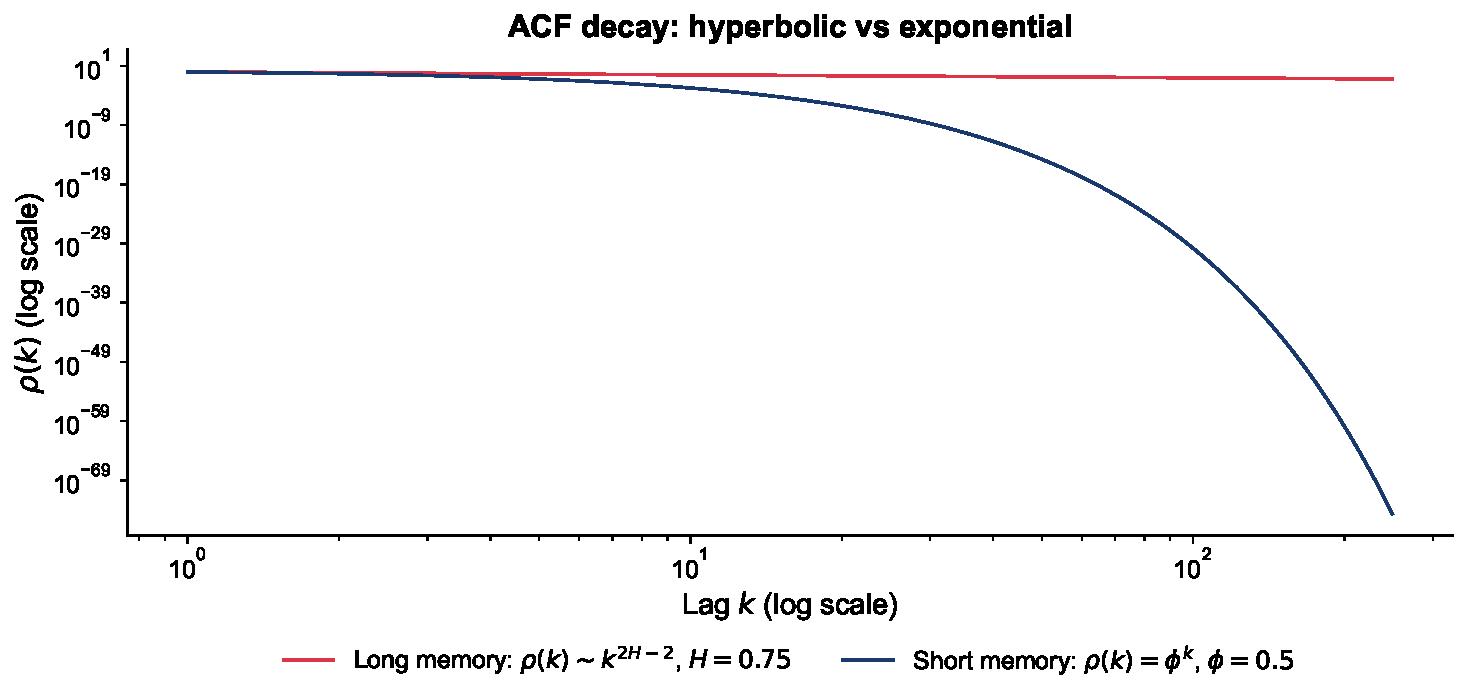
\includegraphics[width=\linewidth,height=4.6cm,keepaspectratio]{ch_fmh_lm_decay.pdf}\\[1pt]
{\scriptsize\textcolor{MediumGray}{\textit{ARFIMA/fBm vs AR(1) pe scală log-log.}}}
\figql{SFM\_ch\_fmh\_extra: lm\_decay}{https://github.com/danpele/SFM/tree/main/Quantlets/SFM_ch_fmh}
\end{column}
\end{columns}
\end{cminipage}
\end{frame}

\slidelevel{PhD}
\begin{frame}[shrink=10]{De la mono- la multifractalitate}
\begin{cminipage}{0.95\textwidth}
\begin{itemize}\setlength{\itemsep}{1pt}
    \item \textbf{Motivație}
    \begin{itemize}\setlength{\itemsep}{0pt}
        \item Un singur $H$ (\textbf{monofractal}) nu surprinde toate regimurile de scalare
    \end{itemize}
    \item \textbf{Construcție}
    \begin{itemize}\setlength{\itemsep}{0pt}
        \item Procesul este \textbf{multifractal} dacă $\E[|X(t)|^q]=c(q)\cdot t^{\tau(q)+1}$ cu $\tau(q)$ \textbf{neliniar} în $q$ (monofractal: $\tau(q)=qH-1$)
        \item \textbf{Spectrul multifractal} $f(\alpha)$ = transformarea Legendre a $\tau(q)$
    \end{itemize}
    \item \textbf{Interpretare}
    \begin{itemize}\setlength{\itemsep}{0pt}
        \item Spectru \textbf{larg} $\Rightarrow$ multifractalitate puternică
        \item Capturează simultan: vol. clustering, cozi grele, intermittency
    \end{itemize}
\end{itemize}
\end{cminipage}
\end{frame}

\slidelevel{PhD}
\begin{frame}[shrink=10]{MMAR: Multifractal Model of Asset Returns}
\begin{cminipage}{0.95\textwidth}
\begin{itemize}\setlength{\itemsep}{1pt}
    \item \textbf{Construcție}
    \begin{itemize}\setlength{\itemsep}{0pt}
        \item Mandelbrot, Fisher, Calvet (1997): \textbf{MMAR}
        \item Log-prețul: $\ln P(t)=B_H(\theta(t))$, cu $\theta(t)=\int_0^t\mu(ds)$ \textbf{trading time multifractal}
    \end{itemize}
    \item \textbf{Avantaje}
    \begin{itemize}\setlength{\itemsep}{0pt}
        \item Captură simultană a 4 fapte stilizate: cozi grele, vol. clustering, memorie lungă, multifractalitate
    \end{itemize}
    \item \textbf{Limitări și extensii}
    \begin{itemize}\setlength{\itemsep}{0pt}
        \item \textbf{Critică}: estimare dificilă; greu de simulat exact
        \item Variantă tractabilă: \textbf{MSM} (Markov-Switching Multifractal, Calvet \& Fisher 2004) --- vezi Anexa~D
    \end{itemize}
\end{itemize}
\end{cminipage}
\end{frame}

\slidelevel{Y3}
\begin{frame}{Recap §6: 3 idei-cheie}
\begin{cminipage}{0.95\textwidth}
\begin{block}{De reținut}
\begin{enumerate}\setlength{\itemsep}{4pt}
    \item fBm = procesul gaussian central al FMH; $H$ controlează memoria, $H=0{,}5$ recuperează mișcarea browniană
    \item ARFIMA = analogul în timp discret, $d=H-1/2$; memoria lungă $\Leftrightarrow$ decadere hiperbolică a $\rho(k)$
    \item Multifractalitatea (MMAR) extinde monofractalul $\to$ spectru $f(\alpha)$ larg, captură mai bună a vol. clustering și cozilor grele
\end{enumerate}
\end{block}
\end{cminipage}
\end{frame}

%#############################################################################
\section{Aplicații empirice: crize, BVB, Bitcoin}
%#############################################################################

\slidelevel{MSc}
\begin{frame}{Ce învățăm aici și de ce contează în finanțe?}
\begin{cminipage}{0.95\textwidth}
\begin{block}{Obiectivele §7}
\begin{itemize}\setlength{\itemsep}{2pt}
    \item Vedem $\hat{H}$ pe clase reale de active (acțiuni, cripto, FX, mărfuri)
    \item Folosim Hurst rolling $\hat{H}_t$ ca \textbf{semnal de criză}
    \item Studii de caz: 1987, GFC (Global Financial Crisis) 2008, COVID-19; analize aprofundate BVB și BTC
    \item Punte: §5 a dat metodele; aici le aplicăm pe date reale
\end{itemize}
\end{block}
\end{cminipage}
\end{frame}

\slidelevel{MSc}
\begin{frame}[shrink=15]{Estimări $\hat{H}$ pe clase de active}
\begin{cminipage}{0.95\textwidth}
\renewcommand{\arraystretch}{1.2}
\centering
\small
\begin{tabular}{lll}
\toprule
\textbf{Clasă / piață} & \textbf{$\hat{H}$ tipic} & \textbf{Metodă} \\
\midrule
S\&P~500 & $0{,}55$--$0{,}62$ & R/S, DFA \\
FTSE~100 & $0{,}53$--$0{,}60$ & DFA \\
DAX~30 & $0{,}54$--$0{,}61$ & R/S, DFA \\
Nikkei~225 & $0{,}52$--$0{,}59$ & DFA \\
\textbf{BET (BVB)} & $\mathbf{0{,}60}$--$\mathbf{0{,}72}$ & R/S, DFA \\
Bitcoin (BTC) & $0{,}50$--$0{,}75$ & DFA, wavelet \\
EUR/USD & $0{,}50$--$0{,}55$ & R/S, DFA \\
Aur (XAU) & $0{,}52$--$0{,}58$ & DFA \\
\bottomrule
\end{tabular}
\vspace{0.15cm}
\begin{itemize}\setlength{\itemsep}{0pt}
    \item Piețe \textbf{dezvoltate}: $\hat{H}$ aproape de $0{,}5$
    \item Piețe \textbf{emergente} (BVB): $\hat{H}\in[0{,}6,\,0{,}7]$ $\Rightarrow$ memorie lungă, eficiență redusă
    \item Forex (cel mai lichid): $\hat{H}$ aproape de EMH
\end{itemize}
\end{cminipage}
\end{frame}

\slidelevel{MSc}
\begin{frame}[shrink=20]{Hurst rolling $\hat{H}_t$ ca semnal de criză}
\begin{cminipage}{0.96\textwidth}
\centering
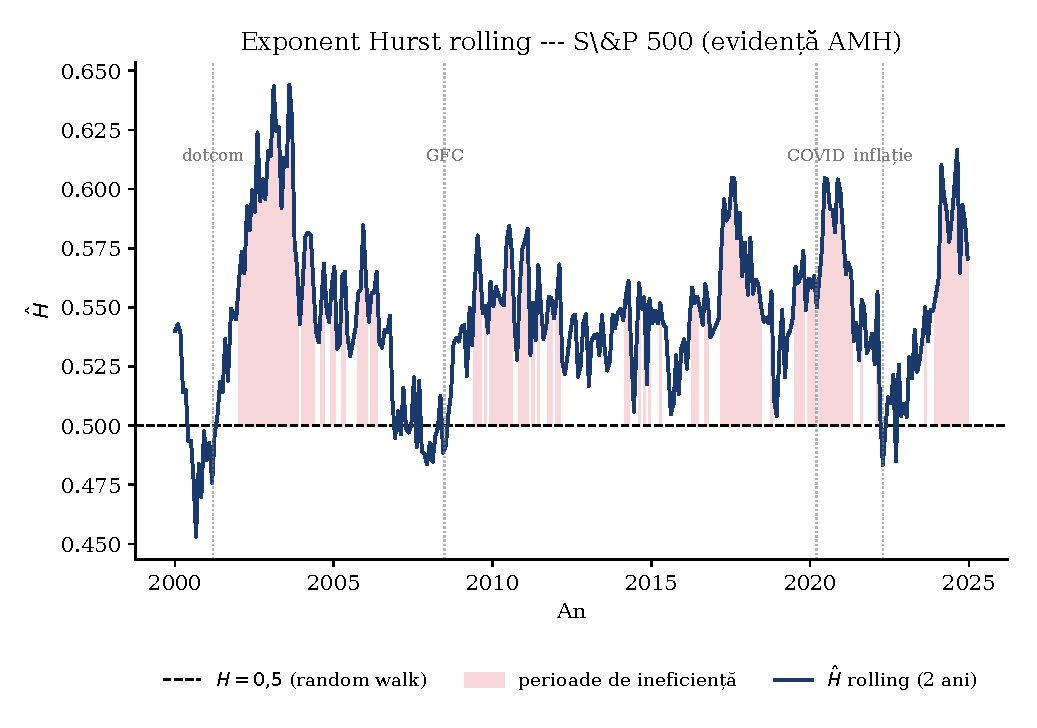
\includegraphics[height=3.8cm,keepaspectratio]{sfm_ch4_rolling_hurst.pdf}\\[1pt]
{\scriptsize\textcolor{MediumGray}{\textit{$\hat{H}_t$ rolling pe S\&P~500, fereastră 252 zile.}}}\\[2pt]
\begin{block}{Observații}
\begin{itemize}\setlength{\itemsep}{0pt}
    \item Scăderi bruște spre $H=0{,}5$ semnalează \textbf{colapsul orizonturilor}
    \item $\hat{H}_t$ ridicat sugerează trend dominant
\end{itemize}
\end{block}
\end{cminipage}
\quantlet{SFM\_ch4\_rolling\_hurst}{https://github.com/danpele/SFM/tree/main/Quantlets/Ch_04/SFM_ch4_rolling_hurst}
\end{frame}

\slidelevel{Y3}
\begin{frame}[shrink=10]{Caz: Black Monday 1987}
\begin{cminipage}{0.95\textwidth}
\begin{columns}[T]
\begin{column}{0.50\textwidth}
\begin{exampleblock}{Evenimente}
\begin{itemize}\setlength{\itemsep}{0pt}
    \item 19 oct 1987: DJIA (Dow Jones Industrial Average) $-22{,}6\%$ într-o zi
    \item Volume $4\times$ media; fără ,,fundamental shock'' clar
    \item Probabilitate sub gauss: $\sim 10^{-50}$
\end{itemize}
\end{exampleblock}
\begin{block}{Cauze}
\begin{itemize}\setlength{\itemsep}{0pt}
    \item Portfolio insurance + program trading
    \item NYSE specialiști copleșiți $\Rightarrow$ \textbf{colaps al orizonturilor}
\end{itemize}
\end{block}
\end{column}
\begin{column}{0.46\textwidth}
\begin{alertblock}{Răspuns reglementar}
\begin{itemize}\setlength{\itemsep}{0pt}
    \item \textbf{Circuit breakers} (NYSE 1988): halt la $-7\%$, $-13\%$, $-20\%$
    \item Sub FMH: pauză = restaurarea diversității orizonturilor
\end{itemize}
\end{alertblock}
\end{column}
\end{columns}
\end{cminipage}
\end{frame}

\slidelevel{MSc}
\begin{frame}[shrink=10]{Caz: Criza Financiară Globală 2008 (GFC)}
\begin{cminipage}{0.95\textwidth}
\begin{columns}[T]
\begin{column}{0.50\textwidth}
\begin{alertblock}{Cronologie}
\begin{itemize}\setlength{\itemsep}{0pt}
    \item aug 2007: BNP Paribas îngheață fonduri MBS
    \item 15 sep 2008: faliment Lehman
    \item Indici globali $-40\%$ în 6 luni; VIX$\to 80$
    \item TARP (Troubled Asset Relief Program) \$700B; QE Fed
\end{itemize}
\end{alertblock}
\end{column}
\begin{column}{0.46\textwidth}
\begin{block}{Citire FMH}
\begin{itemize}\setlength{\itemsep}{0pt}
    \item $\hat{H}$ pe S\&P~500: scade de la $\sim 0{,}55$ la $\sim 0{,}48$
    \item Long-only/value pleacă $\Rightarrow$ rămân HFT
    \item Lichiditate $\downarrow$ abrupt; VaR violations $\gg$ așteptat
\end{itemize}
\end{block}
\end{column}
\end{columns}
\end{cminipage}
\end{frame}

\slidelevel{Y3}
\begin{frame}[shrink=10]{Caz: COVID-19 (martie 2020)}
\begin{cminipage}{0.95\textwidth}
\begin{columns}[T]
\begin{column}{0.50\textwidth}
\begin{exampleblock}{Evenimente}
\begin{itemize}\setlength{\itemsep}{0pt}
    \item 11 mar 2020: OMS declară pandemie
    \item 12 mar: SP500 $-9{,}5\%$; 16 mar: $-12\%$
    \item Cel mai rapid bear market: $-34\%$ în 33 zile
    \item 23 mar: Fed lansează QE infinit
\end{itemize}
\end{exampleblock}
\end{column}
\begin{column}{0.46\textwidth}
\begin{block}{Diagnostic FMH}
\begin{itemize}\setlength{\itemsep}{0pt}
    \item $\hat{H}_t$: colaps de la $\approx 0{,}58$ la $\approx 0{,}40$ în 2 săptămâni
    \item Anti-persistență temporară ($H<0{,}5$): vânzare/cumpărare frenetică
    \item Recuperare V (vs U în 2008)
\end{itemize}
\end{block}
\end{column}
\end{columns}
\end{cminipage}
\end{frame}

\slidelevel{MSc}
\begin{frame}[shrink=10]{Deep-dive: Bursa de Valori București (BVB)}
\begin{cminipage}{0.95\textwidth}
\begin{columns}[T]
\begin{column}{0.50\textwidth}
\begin{itemize}\setlength{\itemsep}{1pt}
    \item \textbf{Date}
    \begin{itemize}\setlength{\itemsep}{0pt}
        \item BET = indice principal (top 21 emitenți)
        \item Studii (Tilfani \& El Boukfaoui 2020; Pele \& Mazurencu 2014): $\hat{H}_{\text{BET}}\in[0{,}60,\,0{,}72]$
    \end{itemize}
    \item \textbf{Interpretare}
    \begin{itemize}\setlength{\itemsep}{0pt}
        \item Mai mare decât piețe dezvoltate $\Rightarrow$ \textbf{memorie lungă, eficiență redusă}
        \item Cauze: lichiditate redusă, retail dominant, concentrare emitenți
    \end{itemize}
\end{itemize}
\end{column}
\begin{column}{0.46\textwidth}
\begin{block}{Promovare la \textit{Emerging Market} (FTSE, sept 2020)}
\begin{itemize}\setlength{\itemsep}{0pt}
    \item $\hat{H}$ pre/post: scade de la $0{,}68$ la $0{,}62$
    \item Volume $\uparrow$, investitori străini $\uparrow$ $\Rightarrow$ diversitate orizonturi $\uparrow$
    \item Confirmă predicția FMH: maturizare $\Rightarrow$ $\hat{H}\to 0{,}5$
\end{itemize}
\end{block}
\end{column}
\end{columns}
\end{cminipage}
\end{frame}

\slidelevel{MSc}
\begin{frame}[shrink=10]{Deep-dive: Bitcoin --- evoluția eficienței}
\begin{cminipage}{0.95\textwidth}
\begin{columns}[T]
\begin{column}{0.55\textwidth}
\begin{itemize}\setlength{\itemsep}{1pt}
    \item \textbf{Cronologie $\hat{H}$}
    \begin{itemize}\setlength{\itemsep}{0pt}
        \item 2010--2014 (nascentă): $\hat{H}_{\text{BTC}}\approx 0{,}70$--$0{,}80$
        \item 2015--2018 (maturizare): $\approx 0{,}55$--$0{,}65$ (CME futures dec~2017)
        \item 2019--prezent: $\approx 0{,}50$--$0{,}55$ (ETF, Exchange-Traded Fund, spot ian 2024)
    \end{itemize}
    \item \textbf{Interpretare}
    \begin{itemize}\setlength{\itemsep}{0pt}
        \item Tranziție clasică: piață ineficientă $\to$ cvasi-eficientă, FX-like
    \end{itemize}
\end{itemize}
\end{column}
\begin{column}{0.42\textwidth}
\begin{alertblock}{Particularități}
\begin{itemize}\setlength{\itemsep}{0pt}
    \item Halving-uri (4 ani) $\Rightarrow$ ciclu fractal suplimentar
    \item Multifractalitate puternică, $f(\alpha)$ larg
    \item Mt.Gox 2014, China ban 2017, Terra/FTX 2022 = reset-uri ale $\hat{H}$
\end{itemize}
\end{alertblock}
\end{column}
\end{columns}
\end{cminipage}
\end{frame}

\slidelevel{MSc}
\begin{frame}[shrink=10]{Template comun pentru studii de caz}
\begin{cminipage}{0.95\textwidth}
\begin{block}{Cele 4 întrebări obligatorii pentru fiecare criză}
\begin{enumerate}\setlength{\itemsep}{3pt}
    \item \textbf{Context}: cronologie, factori declanșatori, magnitudine ($\Delta P,\Delta\sigma,\Delta$ vol.)
    \item \textbf{Ce măsurăm}: serie folosită (frecvență, perioadă), metodă ($\hat{H}$ rolling, DFA, MFDFA)
    \item \textbf{Ce arată $\hat{H}_t$/DFA/MFDFA}: profil $\hat{H}_t$ (drop, anti-persistență, multifractalitate $\Delta\alpha$)
    \item \textbf{Implicație pentru risc}: VaR violations, lichiditate, hedging, reglementare
\end{enumerate}
\end{block}
\begin{exampleblock}{Idee}
\begin{itemize}\setlength{\itemsep}{0pt}
    \item Acest șablon asigură \textbf{comparabilitate} între crize
    \item Conectează diagnosticul fractal cu deciziile de management al riscului
\end{itemize}
\end{exampleblock}
\end{cminipage}
\end{frame}

\slidelevel{Y3}
\begin{frame}{Recap §7: 3 idei-cheie}
\begin{cminipage}{0.95\textwidth}
\begin{block}{De reținut}
\begin{enumerate}\setlength{\itemsep}{4pt}
    \item Piețe dezvoltate au $\hat{H}\approx 0{,}55$; piețe emergente (BVB) $\hat{H}\approx 0{,}65$; cripto au $\hat{H}$ în declin pe măsură ce maturizează
    \item Hurst rolling $\hat{H}_t$ a semnalat 1987, 2008 și COVID-19 prin colaps spre/sub $0{,}5$
    \item BVB ilustrează predicția FMH: lichiditate $\uparrow$ $\Rightarrow$ diversitate orizonturi $\uparrow$ $\Rightarrow$ $\hat{H}\to 0{,}5$
\end{enumerate}
\end{block}
\end{cminipage}
\end{frame}

%#############################################################################
\section{Implicații pentru managementul riscului}
%#############################################################################

\slidelevel{MSc}
\begin{frame}{Ce învățăm aici și de ce contează în finanțe?}
\begin{cminipage}{0.95\textwidth}
\begin{block}{Obiectivele §8}
\begin{itemize}\setlength{\itemsep}{2pt}
    \item De ce \textbf{regula $\sqrt T$} (Basel) eșuează când $H\neq 0{,}5$
    \item VaR și ES (Expected Shortfall) recalibrate cu $T^H$ în loc de $T^{1/2}$
    \item FIGARCH pentru volatilitate cu memorie lungă; pricing sub fBm
    \item Pipeline standard de analiză fractală
\end{itemize}
\end{block}
\end{cminipage}
\end{frame}

\slidelevel{MSc}
\begin{frame}[shrink=10]{De ce contează FMH pentru risk management}
\begin{cminipage}{0.95\textwidth}
\begin{itemize}\setlength{\itemsep}{2pt}
    \item \textbf{Scalarea capitalului}
    \begin{itemize}\setlength{\itemsep}{0pt}
        \item \textbf{Scalarea volatilității} (Basel III, FRTB): regula clasică ,,$\sqrt T$'' presupune $H=0{,}5$
        \item Sub FMH: $\sigma_{T\text{-zile}}=\sigma_{1\text{-zi}}\cdot T^H$
    \end{itemize}
    \item \textbf{Aplicații operaționale}
    \begin{itemize}\setlength{\itemsep}{0pt}
        \item \textbf{Detectare de regim}: $\hat{H}_t$ rolling ca avertizare timpurie
        \item \textbf{Alocarea portofoliului}: $H$ mare $\Rightarrow$ \textit{trend-following}; $H$ mic $\Rightarrow$ \textit{contrarian/value}
        \item \textbf{Multifractal stress testing}: scenarii cu spectru larg $f(\alpha)$
    \end{itemize}
\end{itemize}
\end{cminipage}
\end{frame}

\slidelevel{MSc}
\begin{frame}[shrink=15]{VaR, ES și scalarea riscului sub memorie lungă}
\begin{cminipage}{0.96\textwidth}
\centering
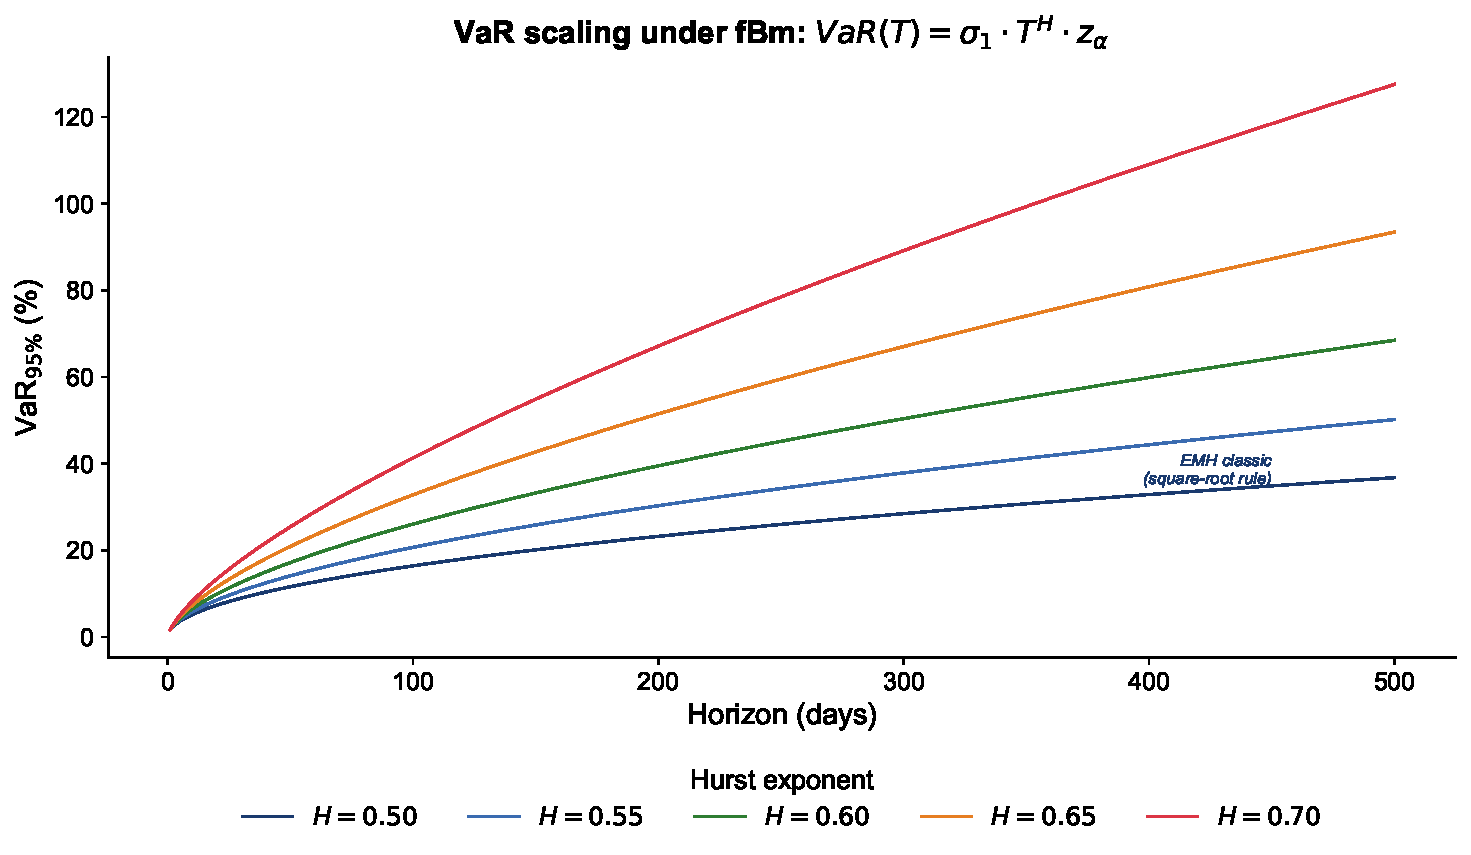
\includegraphics[height=4.6cm,keepaspectratio]{ch_fmh_var_scaling.pdf}\\[2pt]
{\scriptsize\textcolor{MediumGray}{\textit{VaR$_{95\%}$ ca funcție de orizont $T$ pentru valori diferite ale $H$. Sub EMH ($H=0{,}5$), regula $\sqrt T$. FMH cu $H>0{,}5$ produce VaR mai mare pe orizonturi lungi.}}}
\figql{SFM\_ch\_fmh\_extra: var\_scaling}{https://github.com/danpele/SFM/tree/main/Quantlets/SFM_ch_fmh}
\begin{exampleblock}{Idee centrală}
\begin{itemize}\setlength{\itemsep}{0pt}
    \item $\text{VaR}_\alpha(T)\approx \mu T-\sigma T^H z_\alpha$
    \item Eroarea EMH vs FMH crește cu $T$ și cu $H-0{,}5$
\end{itemize}
\end{exampleblock}
\end{cminipage}
\end{frame}

\slidelevel{MSc}
\begin{frame}{De la $\sqrt T$ la $T^H$: numerele concrete}
\begin{cminipage}{0.95\textwidth}
\begin{block}{Factorul de scalare al VaR pe 10 zile (Basel)}
\renewcommand{\arraystretch}{1.25}
\centering
\begin{tabular}{lc}
\toprule
\textbf{Ipoteză} & \textbf{Factor de scalare} \\
\midrule
EMH ($H=0{,}5$): regula $\sqrt T$ & $10^{0{,}5}\approx 3{,}16$ \\
FMH cu $H=0{,}55$ & $10^{0{,}55}\approx 3{,}55$ \quad ($+12\%$) \\
FMH cu $H=0{,}60$ & $10^{0{,}60}\approx 3{,}98$ \quad ($+26\%$) \\
FMH cu $H=0{,}65$ & $10^{0{,}65}\approx 4{,}47$ \quad ($+41\%$) \\
\bottomrule
\end{tabular}
\end{block}
\begin{alertblock}{Implicație practică}
\begin{itemize}\setlength{\itemsep}{0pt}
    \item Pentru BVB ($\hat{H}\approx 0{,}65$): VaR pe 10 zile calculat ca $\sqrt{10}\cdot\sigma_{1d}$ subestimează capitalul cu $\sim 41\%$
\end{itemize}
\end{alertblock}
\end{cminipage}
\end{frame}

\slidelevel{PhD}
\begin{frame}[shrink=10]{FIGARCH: volatilitate cu memorie lungă}
\begin{cminipage}{0.95\textwidth}
\begin{itemize}\setlength{\itemsep}{1pt}
    \item \textbf{Definiție}
    \begin{itemize}\setlength{\itemsep}{0pt}
        \item \textbf{FIGARCH} (Fractionally Integrated GARCH, Baillie--Bollerslev--Mikkelsen, 1996): GARCH(1,1) cu diferențiere fracționară:
        \[
            (1-L)^d\varepsilon_t^2=\omega+\beta(L)v_t,\quad d\in(0,1/2)
        \]
        \item Captură: $\Corr(\varepsilon_t^2,\varepsilon_{t-k}^2)\sim k^{2d-1}$ (decadere hiperbolică a vol.)
    \end{itemize}
    \item \textbf{Alternative și implementare}
    \begin{itemize}\setlength{\itemsep}{0pt}
        \item \textbf{HAR} (Corsi 2009): cascadă pe orizonturi (1d, 5d, 22d) --- conceptual ,,sora FMH'', operațional simplu
        \item Implementare Python: \texttt{arch} (Sheppard)
    \end{itemize}
\end{itemize}
\end{cminipage}
\end{frame}

\slidelevel{PhD}
\begin{frame}{Pricing-ul opțiunilor sub fBm}
\begin{cminipage}{0.95\textwidth}
\begin{itemize}\setlength{\itemsep}{2pt}
    \item \textbf{Problemă}
    \begin{itemize}\setlength{\itemsep}{0pt}
        \item fBm pur \textbf{nu este semimartingală} (Rogers 1997) $\Rightarrow$ permite arbitraj; Black--Scholes nu se aplică direct
    \end{itemize}
    \item \textbf{Soluții moderne}
    \begin{itemize}\setlength{\itemsep}{0pt}
        \item \textbf{Soluții}: mixed fBm (Cheridito 2001), Wick--Itô, \textbf{rough volatility} (Gatheral, Jaisson, Rosenbaum 2018) cu $H\approx 0{,}1$
        \item \textbf{Rough Heston} (El Euch \& Rosenbaum 2019) captează volatility smile mai bine pe orizonturi scurte
    \end{itemize}
    \item \textbf{Referințe}
    \begin{itemize}\setlength{\itemsep}{0pt}
        \item Detalii și formule complete în Anexa~D
    \end{itemize}
\end{itemize}
\end{cminipage}
\end{frame}

\slidelevel{Y3}
\begin{frame}[shrink=10]{Pipeline standard de analiză fractală}
\begin{cminipage}{0.95\textwidth}
\begin{block}{Pipeline 6 pași: data $\to$ $\hat{H}$ $\to$ regim $\to$ risc}
\begin{enumerate}\setlength{\itemsep}{2pt}
    \item \textbf{Data}: log-randamente $r_t=\ln P_t-\ln P_{t-1}$
    \item \textbf{Estimare} $\hat{H}$ prin DFA-1 (sau Lo R/S pentru test formal)
    \item \textbf{Test} $H_0:H=0{,}5$ prin Variance Ratio
    \item \textbf{Verificare regim}: $\hat{H}_t$ rolling + Bai--Perron \textit{breakpoint}
    \item \textbf{Multifractal} (opțional): MFDFA pentru $h(q),f(\alpha)$
    \item \textbf{Risc}: VaR/ES cu scalare $T^H$; alocare în funcție de regim
\end{enumerate}
\end{block}
\end{cminipage}
\end{frame}

\slidelevel{Y3}
\begin{frame}{Recap §8: 3 idei-cheie}
\begin{cminipage}{0.95\textwidth}
\begin{block}{De reținut}
\begin{enumerate}\setlength{\itemsep}{4pt}
    \item Sub FMH: $\sigma(T)=\sigma(1)T^H$ în loc de $\sqrt T$; eroarea VaR Basel poate ajunge la $20$--$40\%$ pentru $H\in[0{,}55,\,0{,}65]$
    \item FIGARCH/HAR pentru memorie lungă în volatilitate; rough volatility ($H\approx 0{,}1$) pentru opțiuni
    \item Pipeline operațional: DFA $\to$ test $H=0{,}5$ $\to$ rolling $\to$ MFDFA $\to$ recalibrare risc
\end{enumerate}
\end{block}
\end{cminipage}
\end{frame}

%#############################################################################
\section{Concluzii și întrebări de examen}
%#############################################################################

\slidelevel{Y3}
\begin{frame}[shrink=10]{Concluzii: 5 idei-cheie}
\begin{cminipage}{0.95\textwidth}
\begin{block}{Mesajele finale ale Cap.~10}
\begin{enumerate}\setlength{\itemsep}{4pt}
    \item \textbf{EMH e utilă dar incompletă}: nu explică memoria lungă, cozile grele și crahurile
    \item \textbf{Piețele sunt scalare} (fractale statistic): $D=2-H$, $\sigma(\Delta)=\sigma(1)\Delta^H$
    \item \textbf{Hurst} $H$ = măsură operațională a memoriei; $\hat{H}$ se estimează prin R/S, DFA, MFDFA
    \item \textbf{FMH = colapsul orizonturilor} explică crahurile (1987, 2008, COVID); $\hat{H}_t$ ca semnal de avertizare timpurie
    \item \textbf{Scalarea fractală schimbă VaR/ES}: regula $\sqrt T$ subestimează capitalul când $H>0{,}5$
\end{enumerate}
\end{block}
\end{cminipage}
\end{frame}

\slidelevel{Y3}
\begin{frame}[shrink=10]{Ce trebuie să știe studentul la examen}
\begin{cminipage}{0.95\textwidth}
\begin{exampleblock}{Întrebări tip examen}
\begin{enumerate}\setlength{\itemsep}{3pt}
    \item Definiți exponentul Hurst și relația cu dimensiunea fractală $D=2-H$. Ce semnifică $H>0{,}5$, $H=0{,}5$, $H<0{,}5$?
    \item Descrieți algoritmul R/S în 5 pași. Care este corecția Lo (1991) și pentru ce problemă?
    \item Comparați EMH vs FMH în 5 dimensiuni: distribuție, memorie, $H$, mecanism de criză, scalare a volatilității.
    \item Calculați factorul de scalare al VaR pe 10 zile dacă $\hat{H}=0{,}60$. Cu cât diferă față de regula Basel $\sqrt T$?
    \item Explicați conceptul ,,colaps al orizonturilor'' și ilustrați cu COVID-19 (martie 2020).
\end{enumerate}
\end{exampleblock}
\end{cminipage}
\end{frame}

\slidelevel{Y3}
\begin{frame}[shrink=15]{Mulțumesc!}
\begin{cminipage}{0.92\textwidth}
\begin{center}
{\Large\textcolor{IDAred}{\textbf{Ipoteza Pieței Fractale}}}\\[0.1cm]

\includegraphics[height=2.0cm]{ch_fmh_mandelbrot_full.pdf}\\[1pt]
\figql{SFM\_ch\_fmh\_fractals: mandelbrot\_full}{https://github.com/danpele/SFM/tree/main/Quantlets/SFM_ch_fmh}
\end{center}
\vspace{0.05cm}
\begin{alertblock}{Citat de încheiere}
\begin{itemize}\setlength{\itemsep}{0pt}
    \item \textit{,,Markets are turbulent, deceptive, complex, and fractal.''}\hfill {\scriptsize --- Benoît Mandelbrot}
\end{itemize}
\end{alertblock}
\begin{block}{Contact}
\begin{itemize}\setlength{\itemsep}{0pt}
    \item \scriptsize \textbf{Daniel Traian PELE} --- \texttt{danpele@ase.ro}
    \item \scriptsize \textbf{Antoaneta Amza}
\end{itemize}
\end{block}
\end{cminipage}
\end{frame}

%#############################################################################
\appendix
%#############################################################################

%#############################################################################
\section{A. Mandelbrot/Julia detaliat}
%#############################################################################

\slidelevel{Y3}
\begin{frame}[shrink=15]{Mulțimea Mandelbrot}
\begin{cminipage}{0.95\textwidth}
\begin{columns}[T]
\begin{column}{0.48\textwidth}
\begin{defn}[$\mathcal{M}$]
Pentru $c\in\mathbb{C}$, $z_0=0$, $z_{n+1}=z_n^2+c$:
\[
    \mathcal{M}=\{c\in\mathbb{C}:\limsup_n|z_n|<\infty\}.
\]
\end{defn}
\begin{itemize}\setlength{\itemsep}{0pt}
    \item Frontiera $\partial\mathcal{M}$ are $D=2$ (Shishikura 1998)
    \item Autosimilaritate: la zoom apar mini-Mandelbrot-uri
\end{itemize}
\end{column}
\begin{column}{0.50\textwidth}
\centering
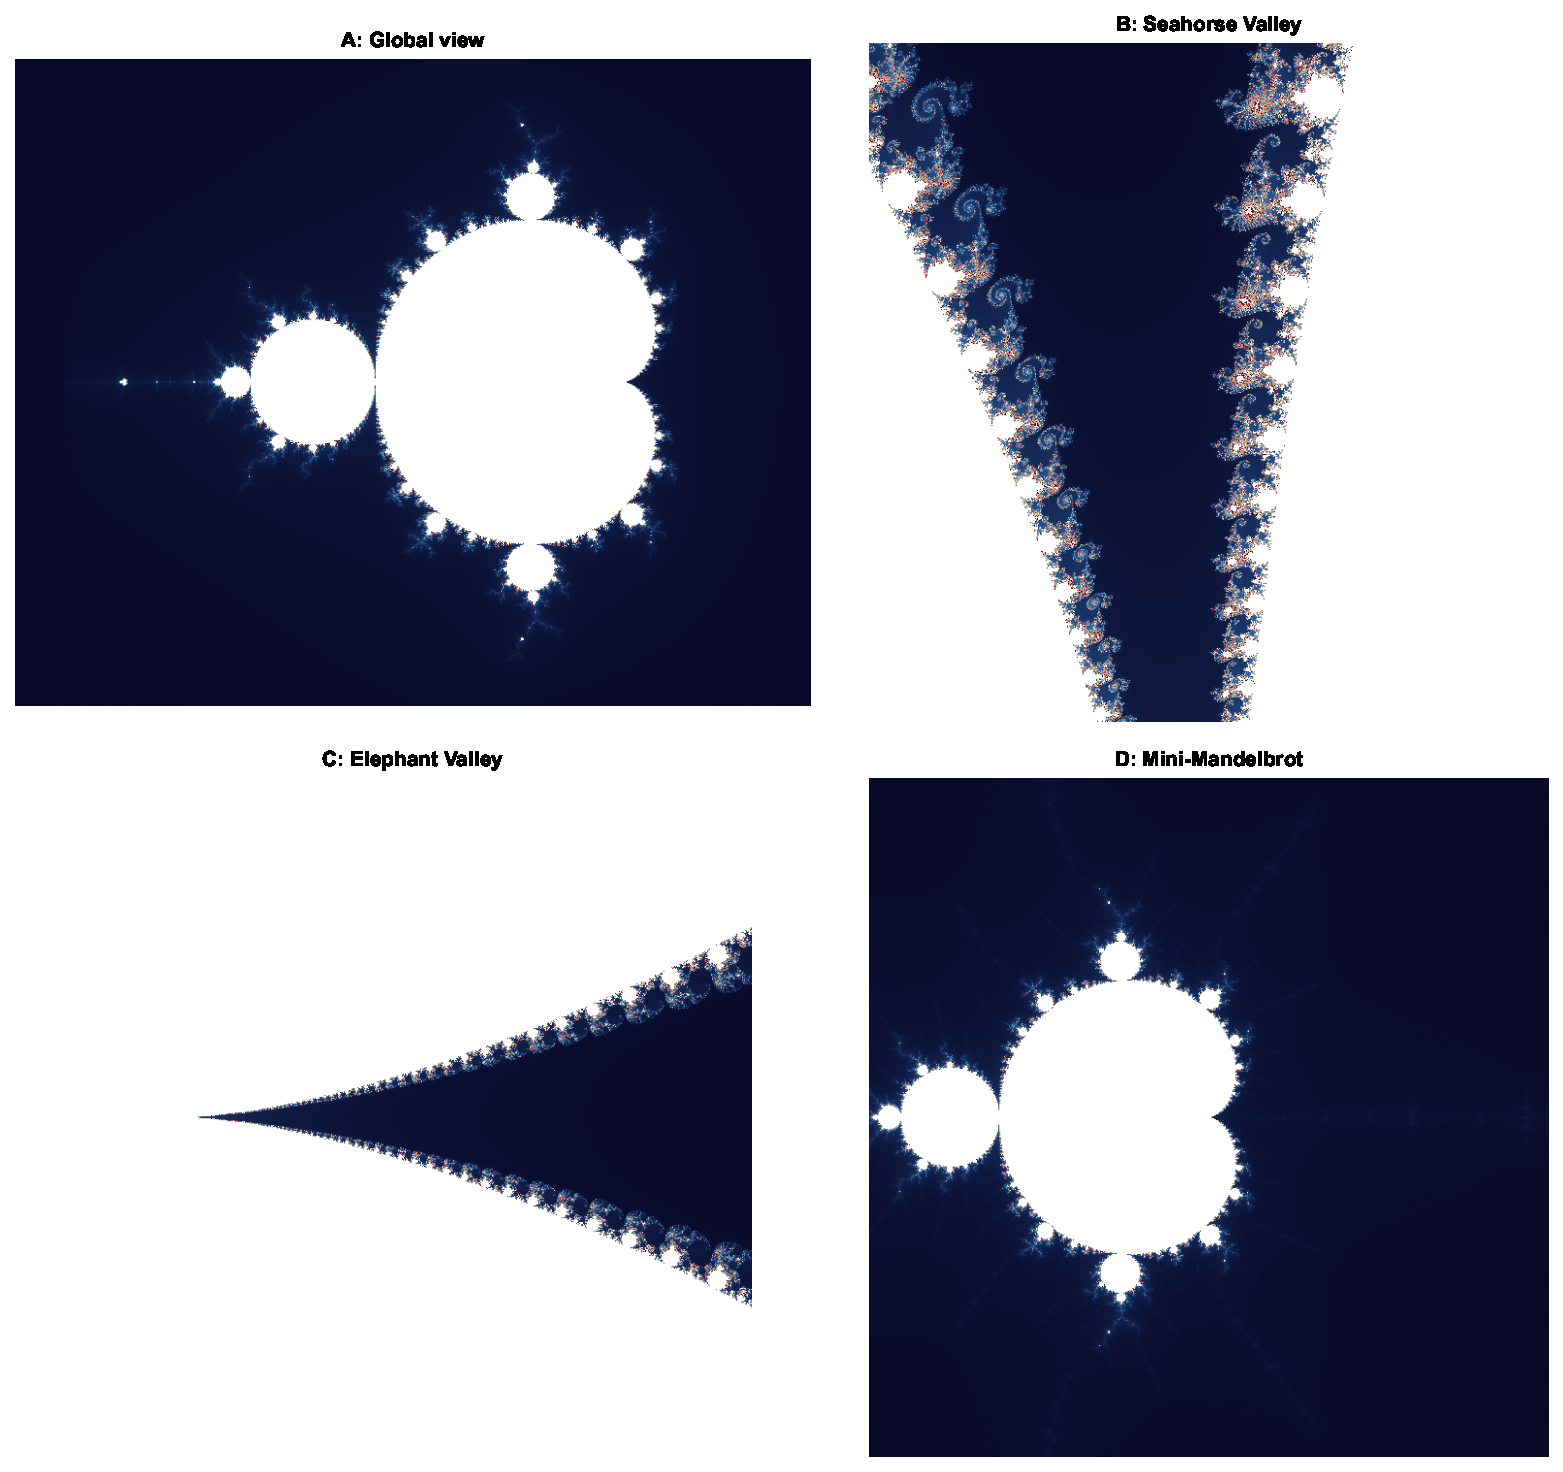
\includegraphics[width=\linewidth,height=4.5cm,keepaspectratio]{ch_fmh_mandelbrot_gallery.pdf}
\figql{SFM\_ch\_fmh\_fractals: mandelbrot\_gallery}{https://github.com/danpele/SFM/tree/main/Quantlets/SFM_ch_fmh}
\end{column}
\end{columns}
\end{cminipage}
\end{frame}

\slidelevel{MSc}
\begin{frame}[shrink=20]{Mulțimile Julia}
\begin{cminipage}{0.95\textwidth}
\begin{columns}[T]
\begin{column}{0.42\textwidth}
\begin{defn}[$\mathcal{J}_c$]
Pentru $c$ fixat, $\mathcal{K}_c=\{z:\{z_n\}\text{ mărginit}\}$. $\mathcal{J}_c=\partial\mathcal{K}_c$.
\end{defn}
\begin{itemize}\setlength{\itemsep}{0pt}
    \item $\mathcal{J}_c$ conexă $\Leftrightarrow$ $c\in\mathcal{M}$
    \item $\mathcal{J}_c$ praf Cantor $\Leftrightarrow$ $c\notin\mathcal{M}$
\end{itemize}
\end{column}
\begin{column}{0.56\textwidth}
\centering
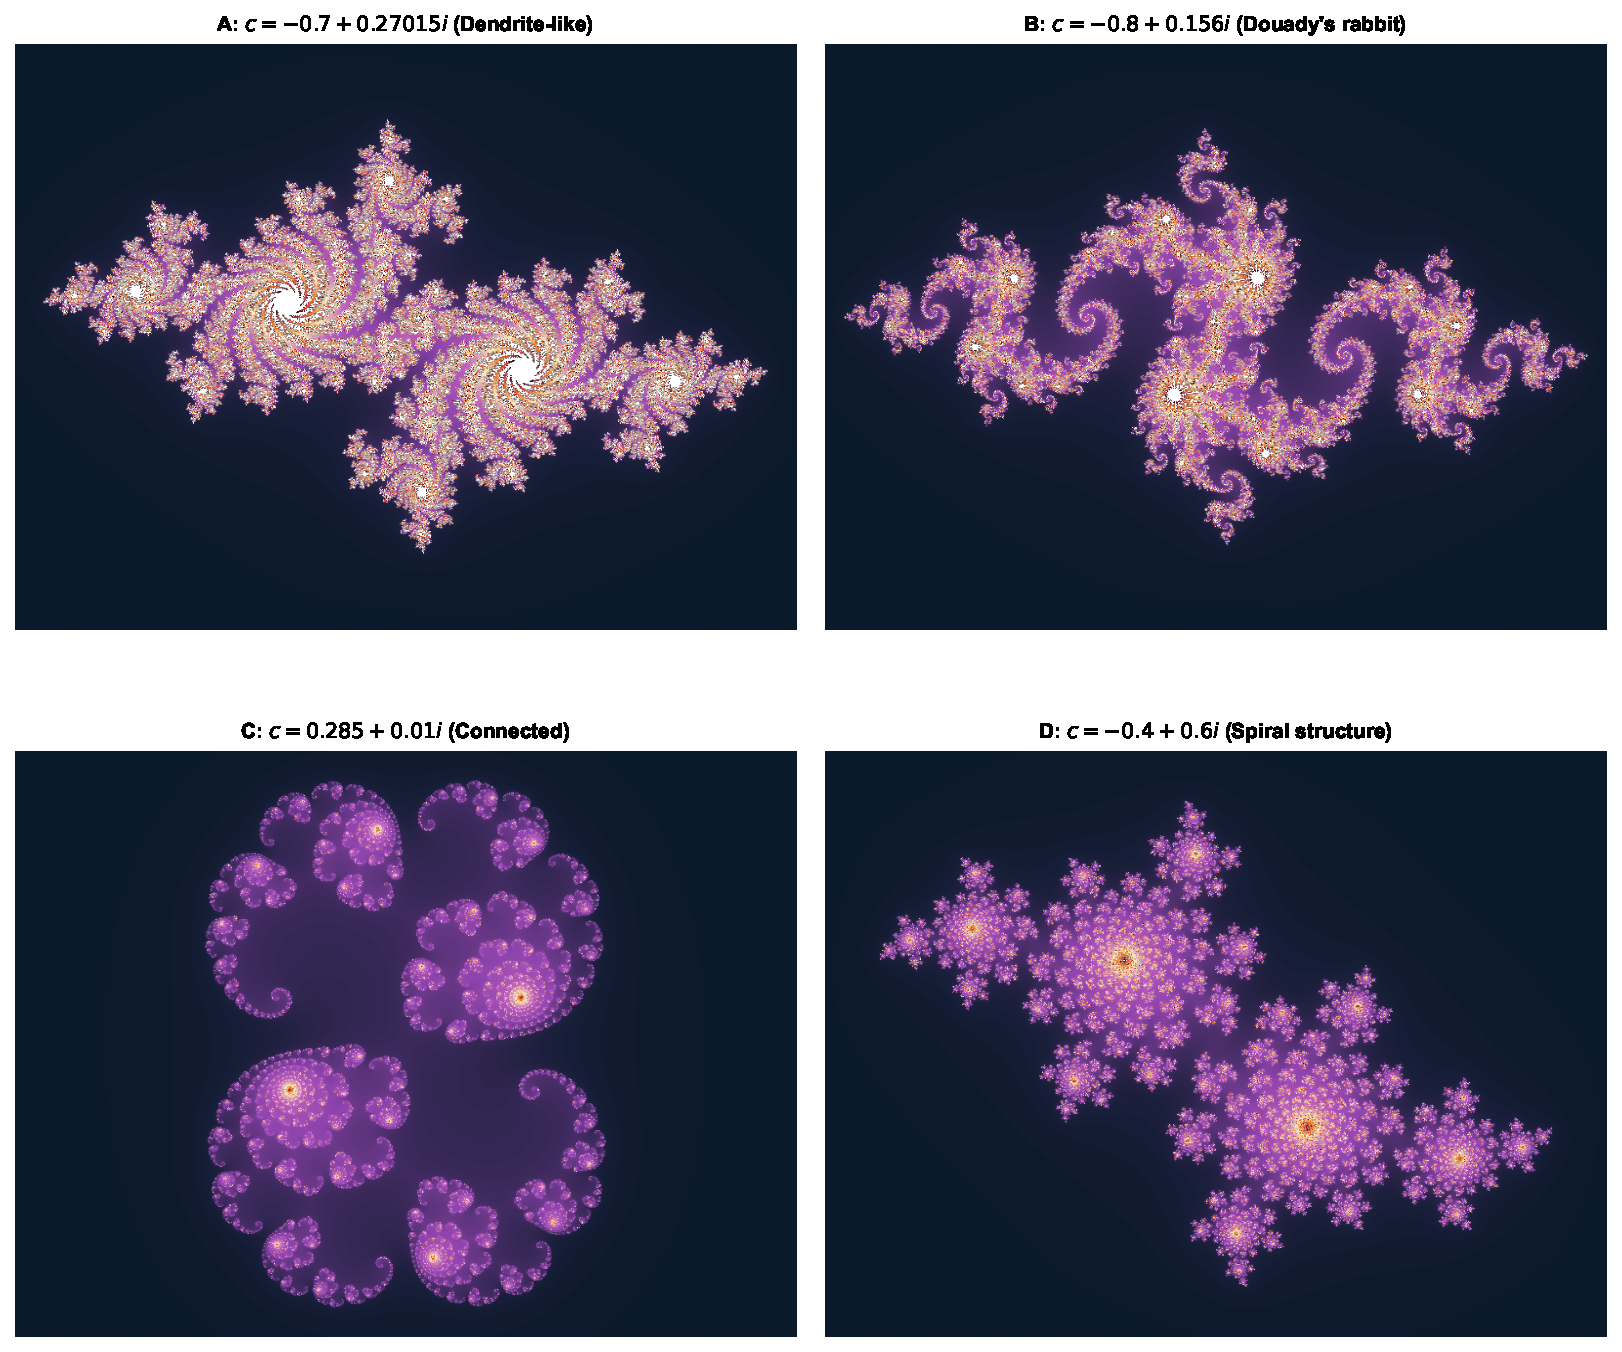
\includegraphics[height=4.0cm,keepaspectratio]{ch_fmh_julia_gallery.pdf}
\figql{SFM\_ch\_fmh\_fractals: julia\_gallery}{https://github.com/danpele/SFM/tree/main/Quantlets/SFM_ch_fmh}
\end{column}
\end{columns}
\end{cminipage}
\end{frame}

\slidelevel{MSc}
\begin{frame}[shrink=15]{Structura Mandelbrot: cardioid și period bulbs}
\begin{cminipage}{0.95\textwidth}
\begin{itemize}\setlength{\itemsep}{1pt}
    \item \textbf{Geometria mulțimii}
    \begin{itemize}\setlength{\itemsep}{0pt}
        \item Componenta principală: \textbf{cardioida} $c(\theta)=\tfrac12 e^{i\theta}(1-\tfrac12 e^{i\theta})$
        \item \textbf{Period bulbs} $D_{p/q}$ atașate la unghiul $2\pi p/q$ $\Rightarrow$ orbită periodică $q$
        \item Filaments \& satellites pe frontieră
    \end{itemize}
    \item \textbf{Rezultate teoretice}
    \begin{itemize}\setlength{\itemsep}{0pt}
        \item Douady \& Hubbard (1982): $\mathcal{M}$ este conexă
        \item Shishikura (1998): $\dim_H(\partial\mathcal{M})=2$
        \item MLC (Mandelbrot Locally Connected): \textbf{problemă deschisă}
    \end{itemize}
\end{itemize}
\end{cminipage}
\end{frame}

\slidelevel{MSc}
\begin{frame}[fragile, shrink=10]{Calculul $\mathcal{M}$: escape time algorithm}
\begin{cminipage}{0.95\textwidth}
\begin{block}{Algoritm}
\begin{itemize}\setlength{\itemsep}{0pt}
    \item Pentru fiecare pixel $c$: $z_0=0$; iterează $z_{n+1}=z_n^2+c$ până $|z_n|>2$ sau $n>N_{\max}$
    \item Smooth coloring: $\mu=n+1-\log\log|z_n|/\log 2$
\end{itemize}
\end{block}
\begin{lstlisting}
def mandelbrot(c, max_iter=300):
    z = 0
    for n in range(max_iter):
        z = z*z + c
        if abs(z) > 2:
            return n + 1 - log(log(abs(z))) / log(2)
    return max_iter
\end{lstlisting}
\end{cminipage}
\end{frame}

\slidelevel{MSc}
\begin{frame}[shrink=10]{Conexiunea Mandelbrot--Julia: dicționarul}
\begin{cminipage}{0.95\textwidth}
\begin{thm}[Julia--Fatou]
Pentru $z_{n+1}=z_n^2+c$: $\mathcal{J}_c$ conexă $\Leftrightarrow$ $c\in\mathcal{M}$; altfel praf Cantor.
\end{thm}
\begin{itemize}\setlength{\itemsep}{0pt}
    \item \textbf{Interpretare globală}
    \begin{itemize}\setlength{\itemsep}{0pt}
        \item $\mathcal{M}$ = atlasul mulțimilor Julia
    \end{itemize}
    \item \textbf{Dicționar local}
    \begin{itemize}\setlength{\itemsep}{0pt}
        \item Cardioid $\Rightarrow$ $\mathcal{J}_c$ simplu conex
        \item Period 2 bulb $\Rightarrow$ $\mathcal{J}_c$ formă de 8
        \item Filamente $\Rightarrow$ $\mathcal{J}_c$ tip dendrite
    \end{itemize}
\end{itemize}
\end{cminipage}
\end{frame}

%#############################################################################
\section{B. Fractali în natură (extins)}
%#############################################################################

\slidelevel{Y3}
\begin{frame}[shrink=10]{Feriga Barnsley}
\begin{cminipage}{0.96\textwidth}
\begin{columns}[T]
\begin{column}{0.42\textwidth}
\begin{itemize}\setlength{\itemsep}{1pt}
    \item \textbf{Construcție}
    \begin{itemize}\setlength{\itemsep}{0pt}
        \item IFS cu 4 transformări afine
        \item Fiecare frunzuliță $\approx$ scalare a întregii ferigi
    \end{itemize}
    \item \textbf{Proprietăți}
    \begin{itemize}\setlength{\itemsep}{0pt}
        \item $D\approx 1{,}82$
        \item Cod genetic minim, complexitate maximă
    \end{itemize}
\end{itemize}
\end{column}
\begin{column}{0.55\textwidth}
\centering

\includegraphics[height=5.6cm]{ch_fmh_barnsley_fern.pdf}
\figql{SFM\_ch\_fmh\_fractals: barnsley\_fern}{https://github.com/danpele/SFM/tree/main/Quantlets/SFM_ch_fmh}
\end{column}
\end{columns}
\end{cminipage}
\end{frame}

\slidelevel{Y3}
\begin{frame}{Copac fractal și fulg Koch (extins)}
\begin{cminipage}{0.96\textwidth}
\begin{columns}[T]
\begin{column}{0.48\textwidth}
\centering

\includegraphics[height=5.4cm]{ch_fmh_fractal_tree.pdf}\\[1pt]
{\scriptsize\textcolor{MediumGray}{\textit{Copac fractal: ramură = copia copacului.}}}
\end{column}
\begin{column}{0.50\textwidth}
\centering
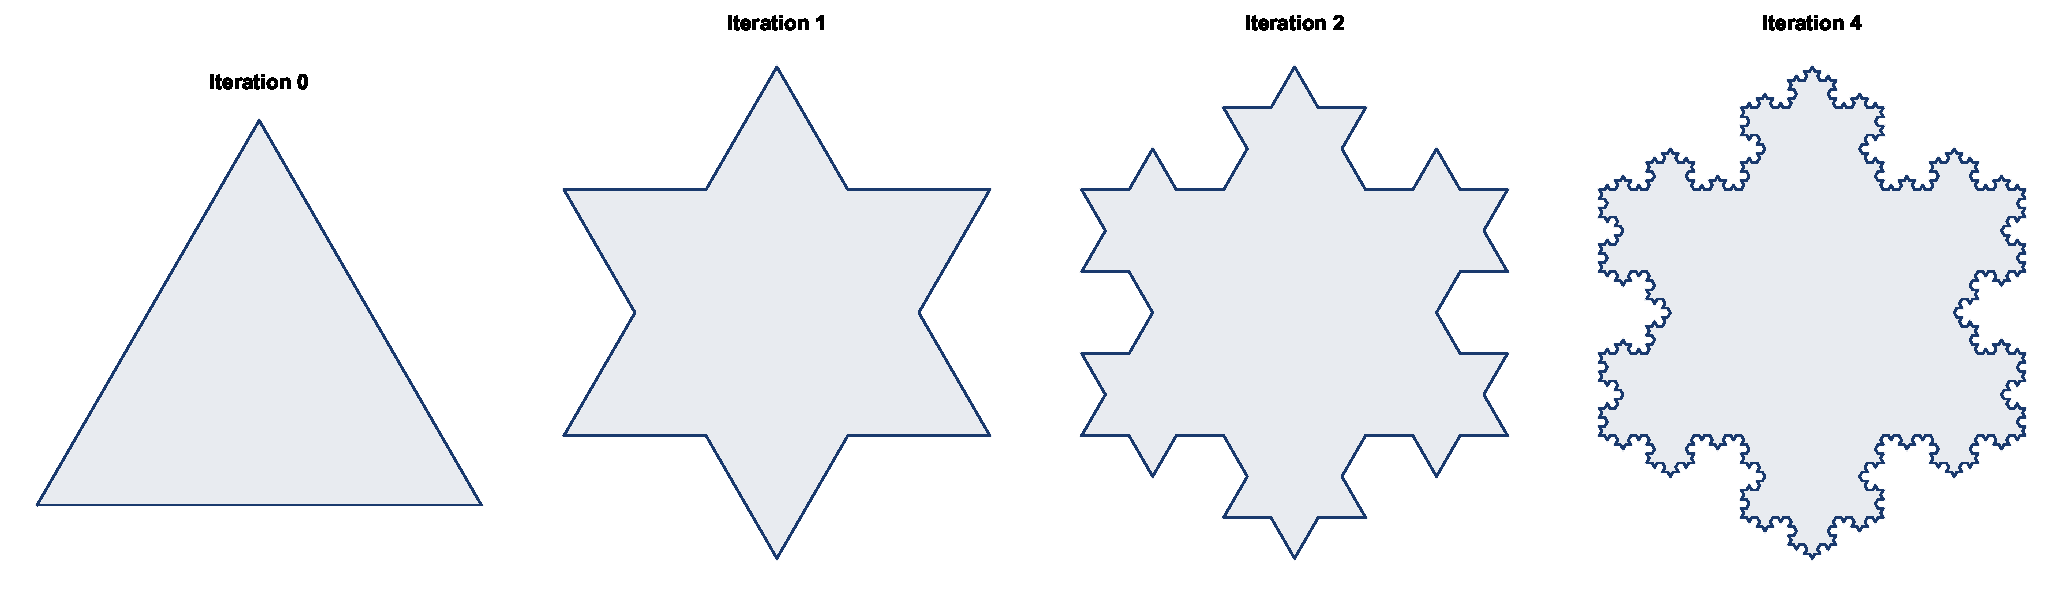
\includegraphics[width=\linewidth]{ch_fmh_koch_snowflake.pdf}\\[1pt]
{\scriptsize\textcolor{MediumGray}{\textit{Fulg Koch, $D\approx 1{,}262$.}}}
\end{column}
\end{columns}
\end{cminipage}
\end{frame}

\slidelevel{Y3}
\begin{frame}{Curba dragonului (Heighway)}
\begin{cminipage}{0.96\textwidth}
\centering
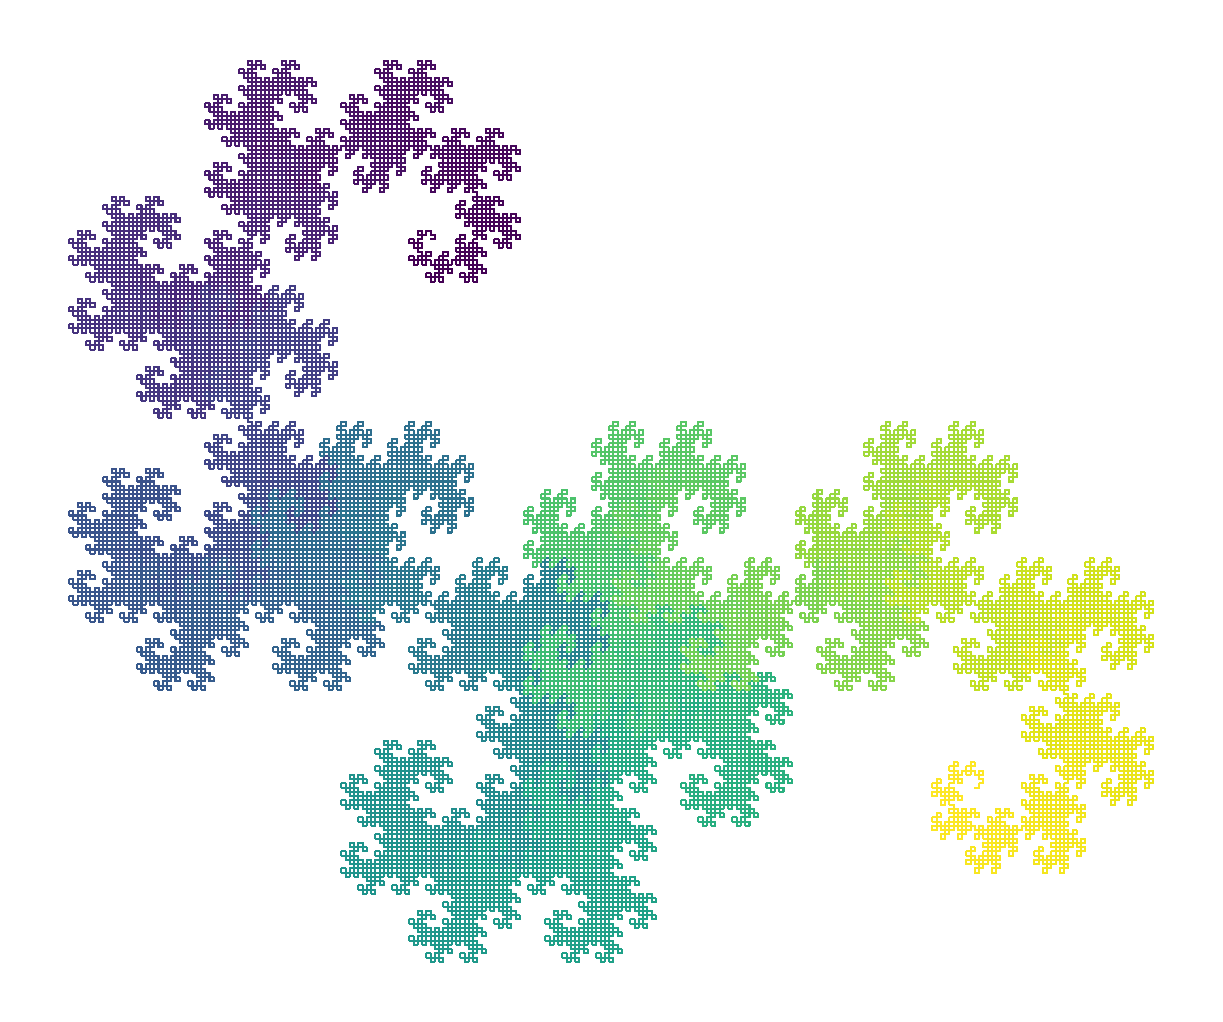
\includegraphics[height=5.6cm]{ch_fmh_dragon_curve.pdf}\\[2pt]
{\scriptsize\textcolor{MediumGray}{\textit{Pliere succesivă; $D\approx 2$.}}}
\figql{SFM\_ch\_fmh\_fractals: dragon\_curve}{https://github.com/danpele/SFM/tree/main/Quantlets/SFM_ch_fmh}
\end{cminipage}
\end{frame}

\slidelevel{Y3}
\begin{frame}[shrink=15]{Fulger / DLA (Diffusion-Limited Aggregation)}
\begin{cminipage}{0.95\textwidth}
\begin{columns}[T]
\begin{column}{0.45\textwidth}
\begin{itemize}\setlength{\itemsep}{1pt}
    \item \textbf{Construcție}
    \begin{itemize}\setlength{\itemsep}{0pt}
        \item Witten \& Sander (1981)
        \item Particule random walk se ,,lipesc'' la primul contact
        \item $D\approx 1{,}71$ (2D); $\approx 2{,}5$ (3D)
    \end{itemize}
    \item \textbf{Aplicații}
    \begin{itemize}\setlength{\itemsep}{0pt}
        \item Apare: fulger, cristale gheață, electrodepunere
        \item Analogia financiară: răspândirea panicii într-o rețea de traderi
    \end{itemize}
\end{itemize}
\end{column}
\begin{column}{0.52\textwidth}
\centering
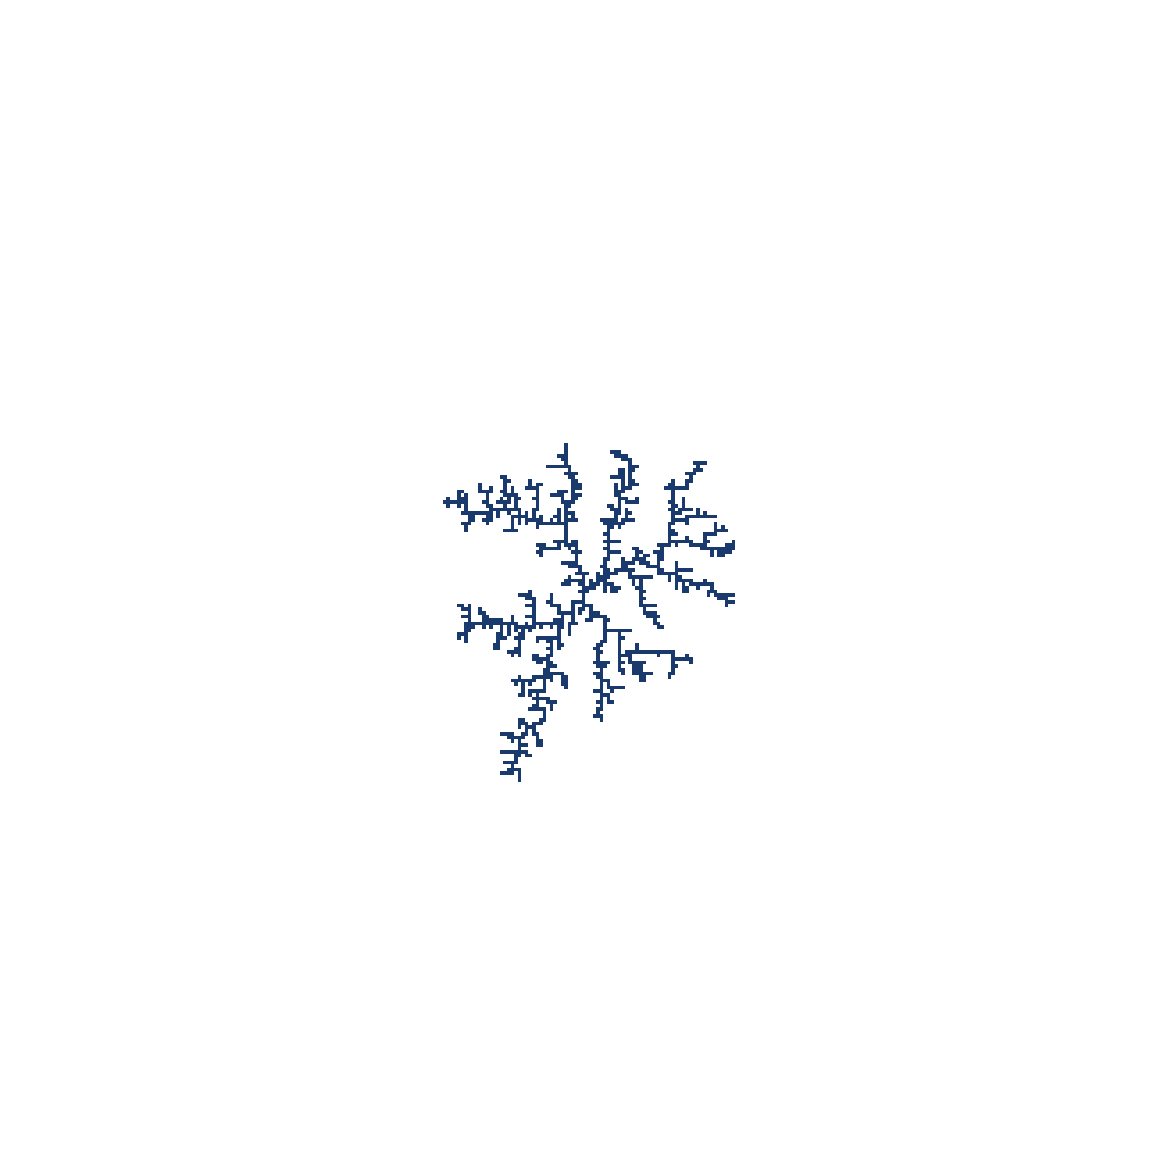
\includegraphics[height=4.0cm,keepaspectratio]{ch_fmh_dla.pdf}
\figql{SFM\_ch\_fmh\_extra: dla}{https://github.com/danpele/SFM/tree/main/Quantlets/SFM_ch_fmh}
\end{column}
\end{columns}
\end{cminipage}
\end{frame}

\slidelevel{Y3}
\begin{frame}[shrink=15]{Rețele de râuri și sisteme circulatorii}
\begin{cminipage}{0.95\textwidth}
\begin{columns}[T]
\begin{column}{0.45\textwidth}
\begin{itemize}\setlength{\itemsep}{1pt}
    \item \textbf{Evidență biologică}
    \begin{itemize}\setlength{\itemsep}{0pt}
        \item Legile Horton (1945)
        \item Bronhii ($\sim$23 nivele), capilare, neuroni
    \end{itemize}
    \item \textbf{Principii și aplicații}
    \begin{itemize}\setlength{\itemsep}{0pt}
        \item Eficiență energetică: ramificare fractală $\Rightarrow$ minimizare transport
        \item West-Brown-Enquist: rata metabolică $\propto M^{3/4}$
        \item Analogia financiară: rețele de plăți, propagare șocuri
    \end{itemize}
\end{itemize}
\end{column}
\begin{column}{0.52\textwidth}
\centering

\includegraphics[height=4.0cm,keepaspectratio]{ch_fmh_river_network.pdf}
\figql{SFM\_ch\_fmh\_extra: river\_network}{https://github.com/danpele/SFM/tree/main/Quantlets/SFM_ch_fmh}
\end{column}
\end{columns}
\end{cminipage}
\end{frame}

\slidelevel{Y3}
\begin{frame}[shrink=10]{Alți fractali din natură}
\begin{cminipage}{0.95\textwidth}
\renewcommand{\arraystretch}{1.2}
\centering
\small
\begin{tabular}{lll}
\toprule
\textbf{Obiect} & \textbf{$D$} & \textbf{Mecanism} \\
\midrule
Coasta Britaniei & $\approx 1{,}25$ & Eroziune \\
Coasta Norvegiei & $\approx 1{,}52$ & Glaciație, fiorduri \\
Munți Alpini & $\approx 1{,}40$ & Eroziune + tectonică \\
Nori cumulus & $1{,}35$--$1{,}40$ & Convecție, turbulență \\
Creier uman & $\approx 2{,}79$ & Maximizare suprafață \\
Bronhii pulmonare & $\approx 2{,}97$ & Schimb O$_2$ \\
Vase de sânge & $\approx 2{,}7$ & West-Brown-Enquist \\
Romanesco & $\approx 2{,}66$ & Spirala Fibonacci \\
Galaxii & $1{,}2$--$2{,}0$ & Gravitație + expansiune \\
\bottomrule
\end{tabular}
\end{cminipage}
\end{frame}

\slidelevel{MSc}
\begin{frame}[shrink=10]{Muzică și limbaj ca fractali}
\begin{cminipage}{0.95\textwidth}
\begin{columns}[T]
\begin{column}{0.50\textwidth}
\begin{block}{Muzică (Voss \& Clarke 1975)}
\begin{itemize}\setlength{\itemsep}{0pt}
    \item Pitch \& loudness: $f(\omega)\sim 1/\omega$
    \item ,,$1/f$ noise'' (zgomot pink)
    \item Bach, Mozart, Beatles: toți în ,,$1/f$''
\end{itemize}
\end{block}
\end{column}
\begin{column}{0.46\textwidth}
\begin{block}{Limbaj (Mandelbrot 1953)}
\begin{itemize}\setlength{\itemsep}{0pt}
    \item Legea Zipf: frecv. $\propto 1/\text{rang}^\alpha$
    \item Coadă grea
    \item Mandelbrot 1953: $f_n=C/(n+\beta)^\alpha$
\end{itemize}
\end{block}
\end{column}
\end{columns}
\begin{exampleblock}{Conexiune cu finanțele}
\begin{itemize}\setlength{\itemsep}{0pt}
    \item Randamentele bursiere urmează aceleași legi de scalare
    \item Cozi grele Pareto, distribuții cu \textit{power-law tails}
\end{itemize}
\end{exampleblock}
\end{cminipage}
\end{frame}

%#############################################################################
\section{C. Cod Python complet}
%#############################################################################

\slidelevel{MSc}
\begin{frame}[fragile, shrink=10]{R/S complet în Python}
\begin{cminipage}{0.95\textwidth}
\begin{lstlisting}
import numpy as np
from scipy import stats

def rs_analysis(x, min_n=10, max_n=None):
    """Estimeaza exponentul Hurst prin analiza R/S."""
    x = np.asarray(x, dtype=float)
    T = len(x)
    if max_n is None:
        max_n = T // 4
    ns = np.unique(np.logspace(np.log10(min_n), np.log10(max_n), 40).astype(int))
    rs_vals = []
    for n in ns:
        n_blocks = T // n
        rs_block = []
        for b in range(n_blocks):
            block = x[b*n : (b+1)*n]
            cumdev = np.cumsum(block - block.mean())
            R = cumdev.max() - cumdev.min()
            S = block.std(ddof=0)
            if S > 1e-15:
                rs_block.append(R / S)
        rs_vals.append(np.mean(rs_block) if rs_block else np.nan)
    log_n = np.log(ns); log_rs = np.log(rs_vals)
    H, _, _, _, _ = stats.linregress(log_n, log_rs)
    return H, ns, rs_vals
\end{lstlisting}
\end{cminipage}
\quantlet{SFM\_ch14\_fractal\_hurst}{https://github.com/danpele/SFM/tree/main/Quantlets/SFM_ch14}
\end{frame}

\slidelevel{MSc}
\begin{frame}[fragile, shrink=10]{DFA complet în Python}
\begin{cminipage}{0.95\textwidth}
\begin{lstlisting}
import numpy as np
from scipy import stats

def dfa(x, order=1, min_n=10, max_n=None):
    """Detrended Fluctuation Analysis (DFA-order)."""
    x = np.asarray(x, dtype=float)
    Y = np.cumsum(x - x.mean())
    N = len(Y)
    if max_n is None: max_n = N // 4
    ns = np.unique(np.logspace(np.log10(min_n), np.log10(max_n), 30).astype(int))
    F = []
    for n in ns:
        nseg = N // n
        rms = []
        for s in range(nseg):
            seg = Y[s*n:(s+1)*n]
            t = np.arange(n)
            p = np.polyfit(t, seg, order)
            trend = np.polyval(p, t)
            rms.append(np.mean((seg - trend)**2))
        F.append(np.sqrt(np.mean(rms)))
    H, _, _, _, _ = stats.linregress(np.log(ns), np.log(F))
    return H, ns, F
\end{lstlisting}
\end{cminipage}
\end{frame}

\slidelevel{PhD}
\begin{frame}[fragile]{Simulare fBm: Davies--Harte}
\begin{cminipage}{0.95\textwidth}
\begin{lstlisting}
from fbm import FBM
f = FBM(n=10000, hurst=0.7, length=1, method='daviesharte')
fbm_path = f.fbm()
fgn_path = f.fgn()
\end{lstlisting}
\begin{itemize}\setlength{\itemsep}{0pt}
    \item Recomandare: \textbf{Davies--Harte} (circulant embedding) pentru $n$ mare; complexitate $O(n\log n)$
    \item Atenție: matricea circulantă trebuie să fie pozitiv definită; pentru $H$ extrem, mărește acoperirea
\end{itemize}
\end{cminipage}
\end{frame}

\slidelevel{MSc}
\begin{frame}[fragile]{Escape time Mandelbrot --- vectorizat NumPy}
\begin{cminipage}{0.95\textwidth}
\begin{lstlisting}
import numpy as np

def mandelbrot_set(width, height, x_min=-2.5, x_max=1.0,
                   y_min=-1.25, y_max=1.25, max_iter=300):
    x = np.linspace(x_min, x_max, width)
    y = np.linspace(y_min, y_max, height)
    C = x[None, :] + 1j * y[:, None]
    Z = np.zeros_like(C); n = np.zeros(C.shape, int)
    for i in range(max_iter):
        mask = np.abs(Z) <= 2
        Z[mask] = Z[mask]**2 + C[mask]
        n[mask] = i
    return n
\end{lstlisting}
\end{cminipage}
\end{frame}

%#############################################################################
\section{D. Demonstrații, tabele și referințe extinse}
%#############################################################################

\slidelevel{Y3}
\begin{frame}[shrink=10]{Context istoric (1872--2004)}
\begin{cminipage}{0.95\textwidth}
\renewcommand{\arraystretch}{1.15}
\centering
\small
\begin{tabular}{lll}
\toprule
\textbf{An} & \textbf{Autor} & \textbf{Contribuție} \\
\midrule
1872 & Weierstrass & Funcție continuă, nicăieri diferențiabilă \\
1883 & Cantor & Mulțimea Cantor \\
1904 & Koch & Curba Koch / fulgul de zăpadă \\
1918 & Julia & Mulțimile Julia \\
1951 & Hurst & Exponentul $H$ \\
1963 & Mandelbrot & Variation of speculative prices \\
1968 & Mandelbrot \& Van Ness & fBm \\
1969 & Mandelbrot \& Wallis & R/S în finanțe \\
1975 & Mandelbrot & Termenul ,,fractal'' \\
1991 & Peters & \textit{Chaos and Order in the Capital Markets} \\
1994 & Peng et al. & DFA \\
1997 & Mandelbrot--Fisher--Calvet & MMAR \\
2004 & Mandelbrot \& Hudson & \textit{(Mis)Behavior of Markets} \\
\bottomrule
\end{tabular}
\end{cminipage}
\end{frame}

\slidelevel{MSc}
\begin{frame}[shrink=10]{Întrebări fundamentale Q1--Q6}
\begin{cminipage}{0.95\textwidth}
\begin{itemize}\setlength{\itemsep}{1pt}
    \item \textbf{Q1.} Sunt randamentele i.i.d.? EMH: Da. Empiric: Nu.
    \item \textbf{Q2.} Există memorie pe termen lung? EMH: Nu, $\rho(k)=0$. Empiric: Da, $H>0{,}5$.
    \item \textbf{Q3.} Crahurile = lebede negre sau eșecuri structurale? EMH: lebede; FMH: structurale.
    \item \textbf{Q4.} Volatilitatea scalează $\sqrt T$ sau $T^H$? EMH: $\sqrt T$. Empiric: $T^H$, $H\in[0{,}55,\,0{,}65]$.
    \item \textbf{Q5.} Auto-similaritate între scale? EMH: aproximativ. FMH: da, statistic.
    \item \textbf{Q6.} Mai multe regimuri de scalare? EMH: nu. Empiric: spectrul $f(\alpha)$ larg.
\end{itemize}
\end{cminipage}
\end{frame}

\slidelevel{Y3}
\begin{frame}[shrink=10]{Edgar Peters: pionier al FMH}
\begin{cminipage}{0.95\textwidth}
\begin{itemize}\setlength{\itemsep}{1pt}
    \item \textbf{Biografie}
    \begin{itemize}\setlength{\itemsep}{0pt}
        \item Edgar E.~Peters (1952--), economist și manager fonduri (PanAgora)
    \end{itemize}
    \item \textbf{Lucrări principale}
    \begin{itemize}\setlength{\itemsep}{0pt}
        \item Peters (1991): \textit{Chaos and Order in the Capital Markets}
        \item Peters (1994): \textit{Fractal Market Analysis} --- carte tehnică
    \end{itemize}
    \item \textbf{Contribuții și critică}
    \begin{itemize}\setlength{\itemsep}{0pt}
        \item Contribuții: R/S aplicat pe DJIA/SP500, conceptul de \textit{cycle length}, ipoteza diversității orizonturilor
        \item Critică ulterioară (Lo 1991): rezultatele R/S clasice instabile $\Rightarrow$ validate ulterior prin DFA și wavelet
    \end{itemize}
\end{itemize}
\end{cminipage}
\end{frame}

\slidelevel{MSc}
\begin{frame}[shrink=10]{Modelul de procesare a informației}
\begin{cminipage}{0.95\textwidth}
\begin{itemize}\setlength{\itemsep}{1pt}
    \item \textbf{Construcție}
    \begin{itemize}\setlength{\itemsep}{0pt}
        \item Reacția pe orizont $h$: $\text{Reacția}_h(t)=w_h\cdot I(t)\cdot \text{Discount}_h(\tau)$
        \item Day trader: discount rapid; pension fund: discount lent
    \end{itemize}
    \item \textbf{Implicații}
    \begin{itemize}\setlength{\itemsep}{0pt}
        \item Stabilitate $\Leftrightarrow$ $w_h$ distribuție largă; instabilitate $\Leftrightarrow$ orizonturi sincronizate
        \item Conexiune cu \textbf{difuziune anomală}: $\langle x^2(t)\rangle\sim t^{2H}$, $H\neq 0{,}5$
    \end{itemize}
\end{itemize}
\end{cminipage}
\end{frame}

\slidelevel{MSc}
\begin{frame}[shrink=10]{Microstructura pieței și FMH}
\begin{cminipage}{0.95\textwidth}
\begin{itemize}\setlength{\itemsep}{1pt}
    \item Componente la nivel microstructural:
    \begin{itemize}\setlength{\itemsep}{0pt}
        \item Market makers (HFT, ms): oferă lichiditate
        \item Informed traders (min--ore): exploatează informația
        \item Liquidity traders (zile): cash needs
        \item Long-term investors (luni--ani): valoarea fundamentală
    \end{itemize}
    \item \textbf{Bid-ask spread} ca indicator de stres
    \item \textbf{Order flow imbalance}: măsură directă a colapsului orizonturilor
    \item Lead-lag (Epps 1979), volume--volatility (Karpoff 1987), realized vol. (Andersen et al. 2003)
\end{itemize}
\end{cminipage}
\end{frame}

\slidelevel{MSc}
\begin{frame}[shrink=10]{Bridging FMH cu finanțele comportamentale}
\begin{cminipage}{0.95\textwidth}
\begin{block}{De ce orizonturile colapsează?}
\begin{itemize}\setlength{\itemsep}{0pt}
    \item Loss aversion (Kahneman--Tversky): pierderile dor de $2\times$
    \item Herding (DeMarzo et al. 2003)
    \item Disposition effect, recency bias
    \item Sub stres, biasele sincronizează orizonturile $\Rightarrow$ colaps fractal
\end{itemize}
\end{block}
\begin{exampleblock}{Sinteza FMH+AMH (Adaptive Market Hypothesis)+Behavioral}
\begin{itemize}\setlength{\itemsep}{0pt}
    \item Piețele oscilează între eficiență cvasi-completă și ineficiență
    \item Toate observabile prin $\hat{H}_t$ variabil
\end{itemize}
\end{exampleblock}
\end{cminipage}
\end{frame}

\slidelevel{Y3}
\begin{frame}[shrink=10]{Lichiditate și diversitate}
\begin{cminipage}{0.95\textwidth}
\begin{itemize}\setlength{\itemsep}{1pt}
    \item 4 dimensiuni ale lichidității: tightness, depth, resiliency, immediacy
    \item Sub FMH: toate depind de \textbf{diversitatea orizonturilor}
    \item Indicatori de stres:
    \begin{itemize}\setlength{\itemsep}{0pt}
        \item Amihud illiquidity ratio: $|r_t|/V_t$
        \item Kyle's lambda: price impact / volum
        \item VIX, TED spread
    \end{itemize}
    \item Politici: BC ca ,,artificial diversity providers'' (QE, intervenții pe obligațiuni/ETF-uri)
\end{itemize}
\end{cminipage}
\end{frame}

\slidelevel{MSc}
\begin{frame}[shrink=10]{Long-memory: regime shifts vs memorie reală}
\begin{cminipage}{0.95\textwidth}
\begin{block}{Critică metodologică}
\begin{itemize}\setlength{\itemsep}{0pt}
    \item Granger \& Ding (1996): nonliniaritate $\Rightarrow$ \textit{spurious} long memory
    \item Diebold \& Inoue (2001): regime shifts pot mima fBm
    \item Mikosch \& Stărică (2004): \textit{structural breaks} $\Rightarrow$ \textit{spurious} LM
\end{itemize}
\end{block}
\begin{exampleblock}{Diagnostic}
\begin{itemize}\setlength{\itemsep}{0pt}
    \item (a) $\hat{H}$ rolling
    \item (b) Bai--Perron breakpoint
    \item (c) DFA pe reziduuri post-detrending
\end{itemize}
\end{exampleblock}
\end{cminipage}
\end{frame}

\slidelevel{MSc}
\begin{frame}{FMH vs AMH (Lo 2004)}
\begin{cminipage}{0.96\textwidth}
\renewcommand{\arraystretch}{1.18}
\centering
\scriptsize
\begin{tabular}{llll}
\toprule
\textbf{Aspect} & \textbf{EMH} & \textbf{FMH} & \textbf{AMH} \\
\midrule
Mecanism & Preferințe raționale & Orizonturi multiple & Competiție evolutivă \\
Eficiență & Mereu & Lichiditate ridicată & Context-dependent \\
Randamente & i.i.d. & Autosimilare $H\neq 0{,}5$ & Adaptive \\
Predictibilitate & Zero & Regimuri (mono/multi) & Variabilă în timp \\
Test primar & Variance ratio & Hurst/DFA + stab. regim & Rolling Sharpe \\
\bottomrule
\end{tabular}
\vspace{0.15cm}
\begin{alertblock}{Notă}
\begin{itemize}\setlength{\itemsep}{0pt}
    \item FMH și AMH \textbf{nu se exclud reciproc}
    \item Sunt două lentile complementare (Khuntia \& Pattanayak 2018)
\end{itemize}
\end{alertblock}
\end{cminipage}
\end{frame}

\slidelevel{MSc}
\begin{frame}[shrink=10]{Horizon collapse: derivare formală}
\begin{cminipage}{0.95\textwidth}
\begin{block}{Setup}
\begin{itemize}\setlength{\itemsep}{0pt}
    \item Investitori indexați după orizont $T_i\in\{1,5,22,252\}$ zile
    \item Pondere cohortă: $w_i$, $\sum w_i=1$
    \item Entropia orizonturilor (proxy didactic): $\mathcal{H}_{\text{horiz}}=-\sum_i w_i\log w_i$
\end{itemize}
\end{block}
\begin{alertblock}{Sub stres}
\begin{itemize}\setlength{\itemsep}{0pt}
    \item $w_i\to\delta_{\text{daytraders}}$ $\Rightarrow$ $\mathcal{H}_{\text{horiz}}\to 0$
    \item Lichiditatea $L(t)\propto \mathcal{H}_{\text{horiz}}$ ca \textbf{proxy didactic, NU lege formală FMH}
\end{itemize}
\end{alertblock}
\quantlet{SFM\_ch10\_horizon\_collapse}{https://github.com/danpele/SFM/tree/main/Quantlets/SFM_ch10}
\end{cminipage}
\end{frame}

\slidelevel{MSc}
\begin{frame}[shrink=10]{Hurst în alte domenii}
\begin{cminipage}{0.95\textwidth}
\renewcommand{\arraystretch}{1.2}
\centering
\small
\begin{tabular}{lll}
\toprule
\textbf{Domeniu} & \textbf{Serie} & \textbf{$\hat{H}$ tipic} \\
\midrule
Hidrologie & Niveluri Nil & $\approx 0{,}73$ \\
Climatologie & Temperaturi globale & $0{,}65$--$0{,}90$ \\
Cardiologie & Inter-bătăi (sănătos) & $\approx 1{,}0$ \\
Cardiologie & Insuf. cardiacă & $\approx 0{,}5$ \\
Neuroștiințe & EEG & $0{,}6$--$0{,}8$ \\
Trafic Internet & Pachete & $\approx 0{,}9$ \\
Astronomie & Galaxii & Multifractal \\
Lingvistică & Zipf & Multifractal \\
Acțiuni & Indici & $0{,}5$--$0{,}65$ \\
Cripto & BTC, ETH & $0{,}50$--$0{,}75$ \\
Forex & EUR/USD & $\approx 0{,}51$ \\
\bottomrule
\end{tabular}
\end{cminipage}
\end{frame}

\slidelevel{PhD}
\begin{frame}[shrink=10]{Variance ratio test, bias și varianța estimatorilor}
\begin{cminipage}{0.95\textwidth}
\begin{itemize}\setlength{\itemsep}{1pt}
    \item Lo \& MacKinlay (1988): $VR(q)=\Var(r_t(q))/(q\,\Var(r_t(1)))$. Sub mers aleator: $VR(q)=1$
    \item Conexiune fGn: $VR(q)\sim q^{2H-1}$ $\Rightarrow$ $\hat{H}=\tfrac12(1+\log VR(q)/\log q)$
    \item Chow--Denning (1993): test multiple-horizon
    \item Bias / varianță (sumar):
    \begin{itemize}\setlength{\itemsep}{0pt}
        \item R/S clasic: bias mare la $H\approx 0{,}5$
        \item DFA-1: bias mic, mediu varianță
        \item Wavelet (WTMM): cea mai bună acuratețe
        \item Whittle: cel mai eficient asimptotic
    \end{itemize}
\end{itemize}
\end{cminipage}
\end{frame}

\slidelevel{PhD}
\begin{frame}[shrink=10]{Wavelet methods (WTMM, wavelet leaders)}
\begin{cminipage}{0.95\textwidth}
\begin{itemize}\setlength{\itemsep}{1pt}
    \item \textbf{Construcție matematică}
    \begin{itemize}\setlength{\itemsep}{0pt}
        \item WTMM (Muzy, Bacry, Arneodo 1991): $T_\psi[X](a,t)=\int X(t')\psi^*((t'-t)/a)dt'$
        \item Funcția de partiție: $Z(q,a)=\sum|T_\psi[X](t_i,a)|^q\sim a^{\tau(q)}$
    \end{itemize}
    \item \textbf{Avantaje și extensii}
    \begin{itemize}\setlength{\itemsep}{0pt}
        \item Avantaje: robust la trenduri, multiscale natural, localizare tempo-frecvență
        \item Wavelet leaders (Jaffard, Lashermes, Abry 2007): variantă mai stabilă numeric
    \end{itemize}
    \item \textbf{Aplicații}
    \begin{itemize}\setlength{\itemsep}{0pt}
        \item Aplicat cu succes pe turbulență, semnale fiziologice, randamente intraday
    \end{itemize}
\end{itemize}
\end{cminipage}
\end{frame}

\slidelevel{MSc}
\begin{frame}[shrink=10]{Densitatea spectrală fGn și autocorelația}
\begin{cminipage}{0.95\textwidth}
\begin{itemize}\setlength{\itemsep}{1pt}
    \item \textbf{Construcție}
    \begin{itemize}\setlength{\itemsep}{0pt}
        \item PSD (Power Spectral Density): $S(\omega)=2\sigma^2\sin^2(\omega/2)\sum_k 1/|2\pi k+\omega|^{2H+1}$
        \item Aproximație $\omega\to 0$: $S(\omega)\sim C_H|\omega|^{1-2H}$
    \end{itemize}
    \item \textbf{Interpretare și estimare}
    \begin{itemize}\setlength{\itemsep}{0pt}
        \item Trei regimuri: $H<0{,}5$ ,,blue noise''; $H=0{,}5$ white; $H>0{,}5$ ,,$1/f$''/red
        \item GPH (Geweke--Porter-Hudak 1983): $\log I(\omega_j)=c-(2H-1)\log\omega_j+\varepsilon_j$
    \end{itemize}
\end{itemize}
\centering
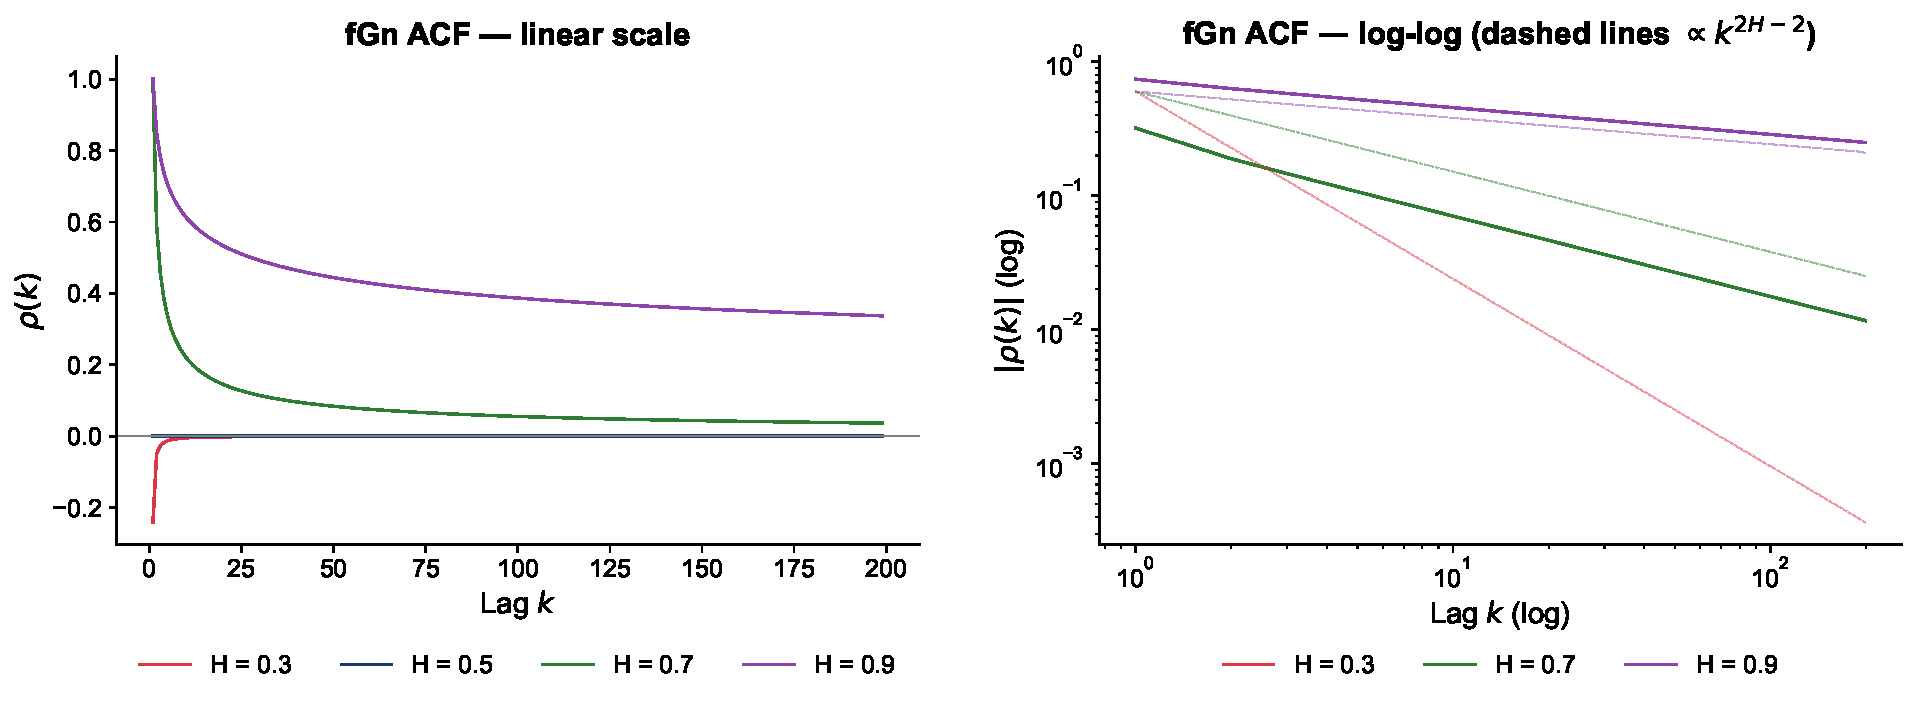
\includegraphics[height=3.4cm,keepaspectratio]{ch_fmh_fgn_acf.pdf}
\figql{SFM\_ch\_fmh\_extra: fgn\_acf}{https://github.com/danpele/SFM/tree/main/Quantlets/SFM_ch_fmh}
\end{cminipage}
\end{frame}

\slidelevel{MSc}
\begin{frame}{Scalarea varianței sub fBm}
\begin{cminipage}{0.96\textwidth}
\centering
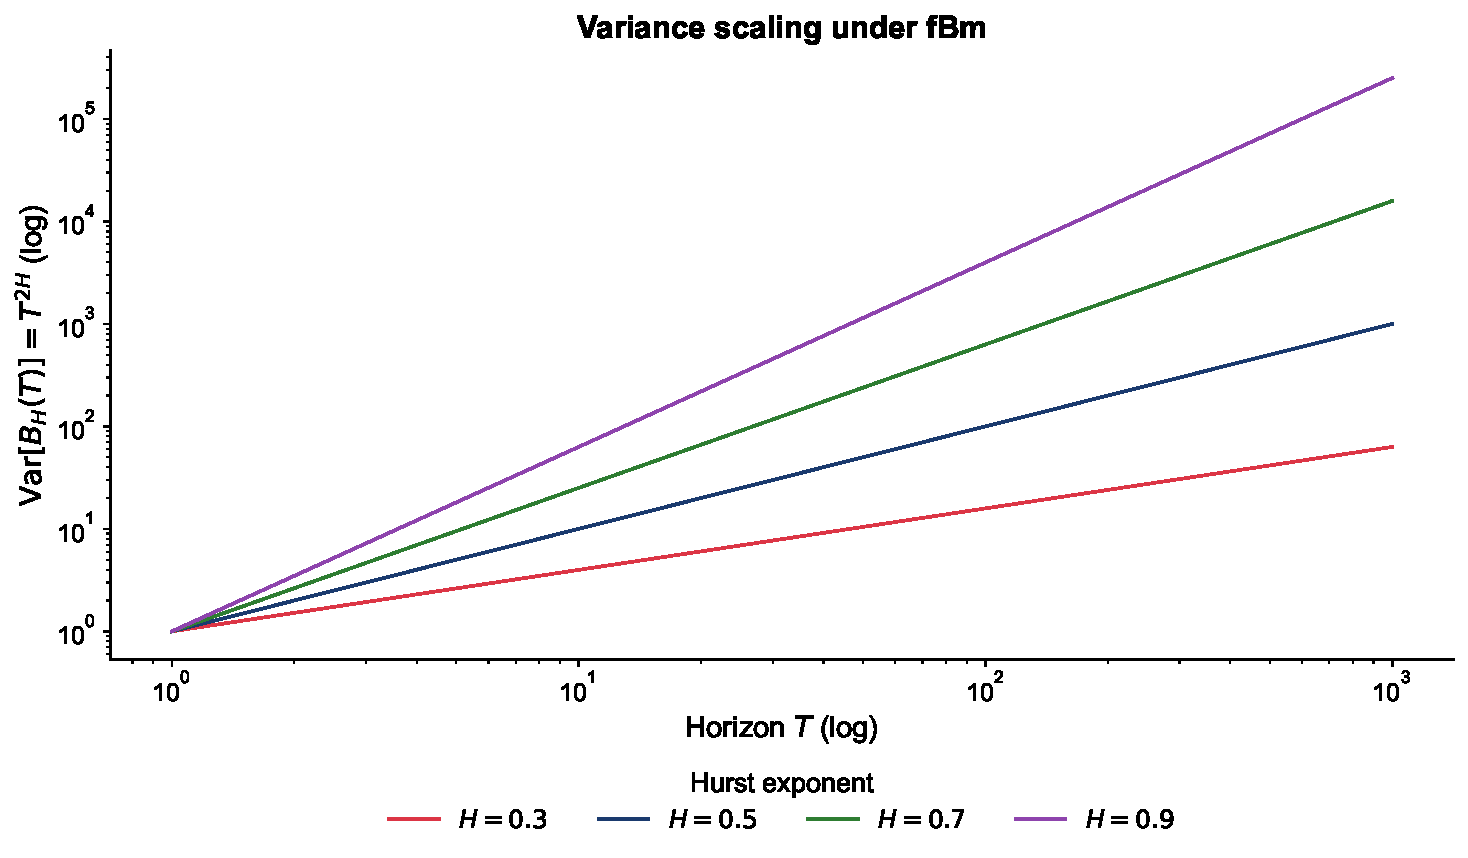
\includegraphics[height=4.6cm,keepaspectratio]{ch_fmh_var_scale_T2H.pdf}\\[2pt]
{\small\textcolor{MediumGray}{\textit{Scalarea $\Var[B_H(T)]=T^{2H}$ în log-log; pantele = $2H$.}}}
\figql{SFM\_ch\_fmh\_extra: var\_scale}{https://github.com/danpele/SFM/tree/main/Quantlets/SFM_ch_fmh}
\end{cminipage}
\end{frame}

\slidelevel{PhD}
\begin{frame}[shrink=10]{Hölder local și cascade multiplicative}
\begin{cminipage}{0.95\textwidth}
\begin{defn}[Hölder pointwise]
$\alpha(t_0)=\sup\{\alpha:|f(t)-P(t-t_0)|\leq C|t-t_0|^\alpha\}$.
\end{defn}
\begin{itemize}\setlength{\itemsep}{0pt}
    \item Pentru fBm: $\alpha(t)=H$ aproape sigur
    \item Pentru multifractali: $\alpha(t)$ variază $\Rightarrow$ spectru $f(\alpha)$
    \item \textbf{Cascade multiplicative} (binomială, lognormală, Calvet--Fisher): redistribuire iterativă a masei
\end{itemize}
\centering
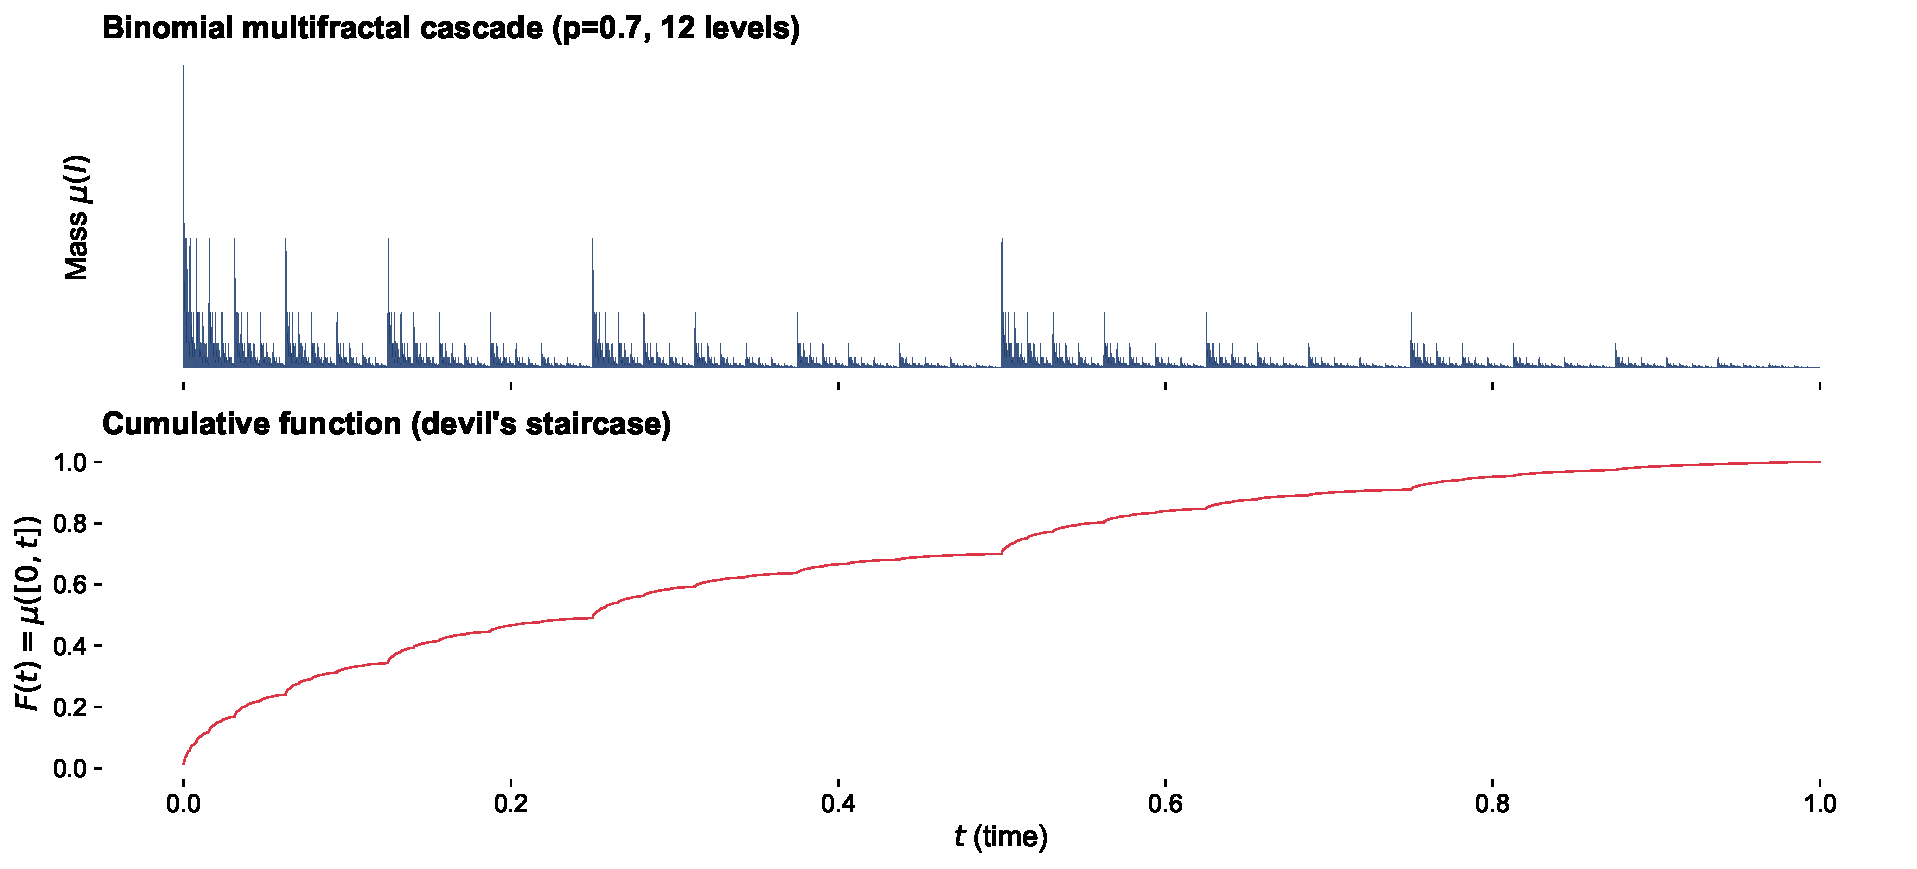
\includegraphics[height=3.0cm,keepaspectratio]{ch_fmh_multi_cascade.pdf}
\figql{SFM\_ch\_fmh\_extra: multi\_cascade}{https://github.com/danpele/SFM/tree/main/Quantlets/SFM_ch_fmh}
\end{cminipage}
\end{frame}

\slidelevel{PhD}
\begin{frame}{Spectrul multifractal $f(\alpha)$}
\begin{cminipage}{0.96\textwidth}
\centering
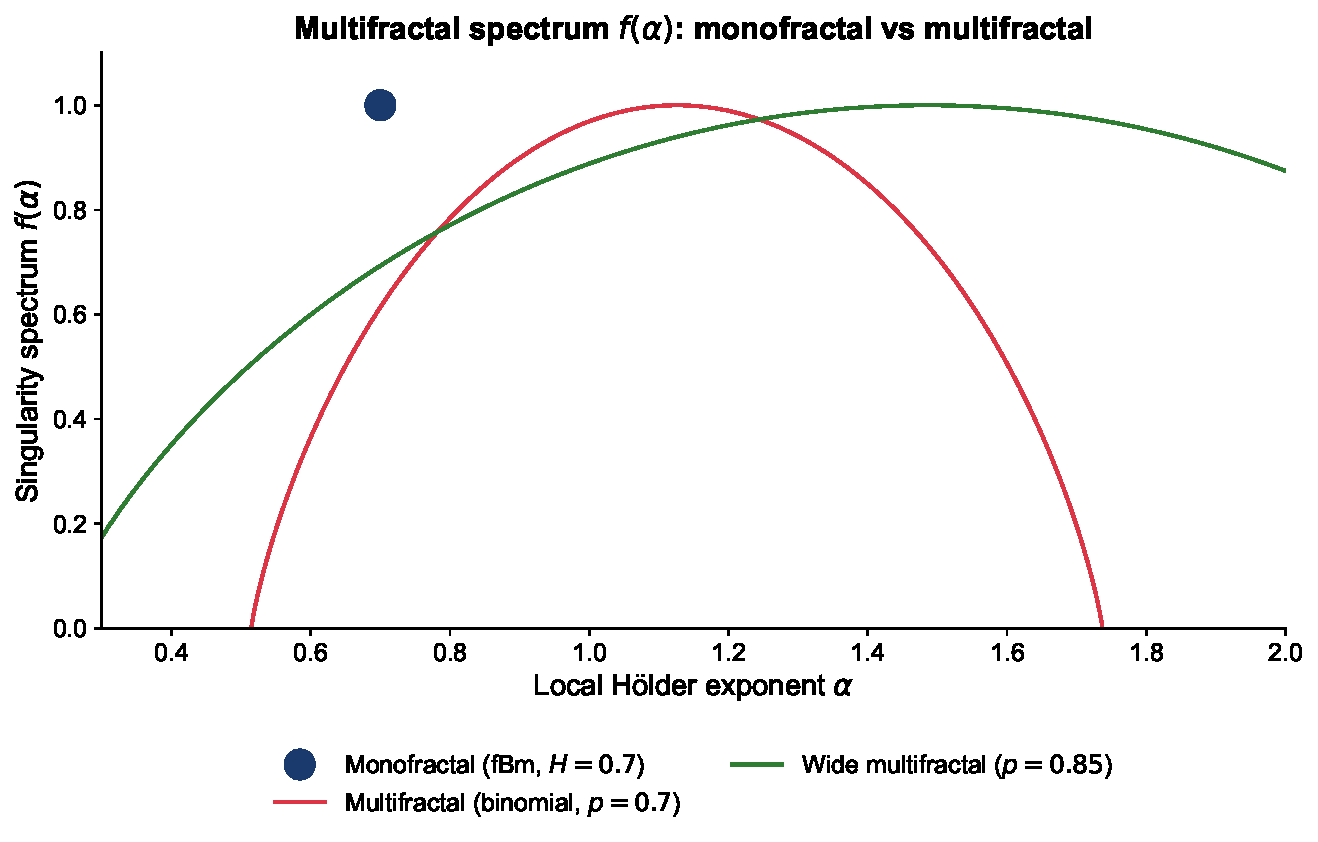
\includegraphics[height=4.4cm,keepaspectratio]{ch_fmh_spectrum.pdf}\\[2pt]
{\scriptsize\textcolor{MediumGray}{\textit{Monofractal: punct $(\alpha=H,\,f=1)$. Multifractal: interval $[\alpha_{\min},\alpha_{\max}]$, $f(\alpha)\leq 1$. Lățimea $\Delta\alpha$ cuantifică multifractalitatea.}}}
\figql{SFM\_ch\_fmh\_extra: spectrum}{https://github.com/danpele/SFM/tree/main/Quantlets/SFM_ch_fmh}
\end{cminipage}
\end{frame}

\slidelevel{PhD}
\begin{frame}[shrink=10]{MMAR: construcție și critică (extins)}
\begin{cminipage}{0.95\textwidth}
\begin{itemize}\setlength{\itemsep}{1pt}
    \item \textbf{Construcție în 2 pași}
    \begin{itemize}\setlength{\itemsep}{0pt}
        \item Pas 1: trading time multifractal $\theta(t)=\int_0^t\mu(ds)$ ($\mu$ = cascadă pozitivă)
        \item Pas 2: $\ln P(t)=B_H(\theta(t))$
    \end{itemize}
    \item \textbf{Proprietăți de scalare}
    \begin{itemize}\setlength{\itemsep}{0pt}
        \item Scalarea momentelor: $\E[|\ln P(t+\tau)-\ln P(t)|^q]\sim\tau^{\tau_X(q)}$, cu $\tau_X(q)=\tau_\theta(qH)-1$
    \end{itemize}
    \item \textbf{Critică și implementări}
    \begin{itemize}\setlength{\itemsep}{0pt}
        \item Critică: estimare empirică dificilă; nu are real-time bine-definit
        \item Implementări: Calvet \& Fisher (2002), Lux (2008)
    \end{itemize}
\end{itemize}
\end{cminipage}
\end{frame}

\slidelevel{PhD}
\begin{frame}[shrink=10]{MSM: Markov-Switching Multifractal (Calvet \& Fisher 2004)}
\begin{cminipage}{0.95\textwidth}
\begin{itemize}\setlength{\itemsep}{1pt}
    \item \textbf{Construcție}
    \begin{itemize}\setlength{\itemsep}{0pt}
        \item Volatility = produsul a $K$ multiplicatori Markov independenți: $\sigma_t^2=\bar\sigma^2\prod_{k=1}^K M_{k,t}$
        \item $M_{k,t}\in\{m_0,2-m_0\}$ cu prob.~$1/2$
        \item Frecvență switch: $\gamma_k=1-(1-\gamma_K)^{(b^{k-K})}$
    \end{itemize}
    \item \textbf{Estimare și performanță}
    \begin{itemize}\setlength{\itemsep}{0pt}
        \item Estimare prin MLE recursivă; bună forecasting; captură multifractal
    \end{itemize}
\end{itemize}
\end{cminipage}
\end{frame}

\slidelevel{MSc}
\begin{frame}[shrink=10]{Aplicații MFDFA și forecasting cu spectru multifractal}
\begin{cminipage}{0.95\textwidth}
\renewcommand{\arraystretch}{1.18}
\centering
\small
\begin{tabular}{llll}
\toprule
\textbf{Piață} & \textbf{$h(2)$} & \textbf{$\Delta\alpha$} & \textbf{Multifractal?} \\
\midrule
S\&P~500 (1990--2024) & $0{,}55$ & $0{,}45$ & moderat \\
DAX~30 & $0{,}54$ & $0{,}42$ & moderat \\
BET (BVB) & $0{,}65$ & $0{,}38$ & slab \\
Bitcoin & $0{,}53$ & $0{,}55$ & puternic \\
EUR/USD & $0{,}51$ & $0{,}30$ & aproape mono \\
Brent oil & $0{,}53$ & $0{,}50$ & puternic \\
\bottomrule
\end{tabular}
\vspace{0.1cm}
\begin{exampleblock}{Forecasting cu features multifractale}
\begin{itemize}\setlength{\itemsep}{0pt}
    \item Calvet \& Fisher (2008): MSM depășește GARCH(1,1) la 10--30 zile
    \item Liu et al. (2020): features MFDFA cresc R$^2$ cu 5--10\% pe XGBoost
    \item Wei et al. (2018): predicție crize prin $\Delta\alpha$ rolling
\end{itemize}
\end{exampleblock}
\end{cminipage}
\end{frame}

\slidelevel{Y3}
\begin{frame}[shrink=10]{Studii de caz suplimentare: 1929, Asia 1997 / LTCM}
\begin{cminipage}{0.95\textwidth}
\begin{block}{Marea Depresiune 1929}
\begin{itemize}\setlength{\itemsep}{0pt}
    \item Sept 1929 max DJIA 381; 24 oct ,,Black Thursday'' $-9\%$; 29 oct ,,Black Tuesday'' $-12\%$
    \item Iulie 1932: minim 41, $-89\%$ față de vârf
    \item Mandelbrot \& Hudson (2004): $\hat{H}\approx 0{,}65\to 0{,}45$ în săptămâna critică
    \item Lecție: \textbf{\textit{margin trading}} ($90\%$ \textit{leverage}) a colapsat orizonturile peste noapte
\end{itemize}
\end{block}
\begin{block}{Asia 1997 + LTCM 1998}
\begin{itemize}\setlength{\itemsep}{0pt}
    \item Asia: Thailanda devalorizează baht-ul (2 iul 1997); $\hat{H}$ pe piețe asiatice: $0{,}68\to 0{,}50$ în 2 săpt
    \item LTCM (Long-Term Capital Management): hedge fund cu modele gaussiene; default rusesc aug 1998 $\Rightarrow$ \$4{,}6B pierderi
    \item Lecție: presupunerea $H=0{,}5$ subestimează \textit{tail risk}
\end{itemize}
\end{block}
\end{cminipage}
\end{frame}

\slidelevel{MSc}
\begin{frame}[shrink=10]{Studii de caz suplimentare: Flash Crash 2010, GameStop 2021, SVB 2023}
\begin{cminipage}{0.95\textwidth}
\begin{block}{Flash Crash (6 mai 2010)}
\begin{itemize}\setlength{\itemsep}{0pt}
    \item 14:32 ET ordin Waddell \& Reed \$4{,}1B E-mini; 14:42 SP500 $-9\%$ în 5 min
    \item \$1 trilion volatilizat și recuperat în 36 min
    \item $\hat{H}_t$ second-by-second: $0{,}55\to 0{,}30$ în 3 min
    \item Reglementare: LULD, single-stock circuit breakers, CAT
\end{itemize}
\end{block}
\begin{block}{GameStop (ian 2021) și SVB (mar 2023)}
\begin{itemize}\setlength{\itemsep}{0pt}
    \item GME $+1500\%$ în 2 săpt; Melvin Capital pierde \$6B; $\hat{H}$ explodează la $0{,}85$ apoi cade la $0{,}30$
    \item SVB (Silicon Valley Bank): bank run digital prin Slack/Twitter, \$42B retrași într-o zi; FDIC închide
    \item Tehnologia accelerează colapsul orizonturilor
\end{itemize}
\end{block}
\end{cminipage}
\end{frame}

\slidelevel{MSc}
\begin{frame}[shrink=10]{Comparație internațională, frecvențe și teste formale}
\begin{cminipage}{0.95\textwidth}
\begin{itemize}\setlength{\itemsep}{1pt}
    \item \textbf{Pattern internațional}
    \begin{itemize}\setlength{\itemsep}{0pt}
        \item Pattern: piețe \textbf{dezvoltate} $\hat{H}\approx 0{,}55$; \textbf{emergente} $\hat{H}\in[0{,}6,\,0{,}7]$
        \item România BET $\approx 0{,}65$, Polonia WIG20 $\approx 0{,}60$, Cehia PX $\approx 0{,}60$
    \end{itemize}
    \item \textbf{Efectul frecvenței}
    \begin{itemize}\setlength{\itemsep}{0pt}
        \item $\hat{H}$ pe \textbf{frecvențe}: în general crește cu agregarea (lunar > zilnic > intraday)
        \item Excepție: cripto au comportament inversat la unele frecvențe $\Rightarrow$ multifractalitate
    \end{itemize}
    \item \textbf{Teste formale}
    \begin{itemize}\setlength{\itemsep}{0pt}
        \item \textbf{Teste formale} pentru $H=0{,}5$: Lo R/S, VR (Variance Ratio), Chow--Denning, GPH, Robinson, Whittle, ELW (Shimotsu--Phillips)
        \item Recomandare: \textbf{minim 3 teste} (e.g.,~Lo + VR + GPH); putere redusă pentru $H\approx 0{,}55$
    \end{itemize}
\end{itemize}
\end{cminipage}
\end{frame}

\slidelevel{MSc}
\begin{frame}[shrink=10]{Detectarea regimurilor folosind $\hat{H}_t$}
\begin{cminipage}{0.95\textwidth}
\begin{itemize}\setlength{\itemsep}{1pt}
    \item Trending (regim de trend): $\hat{H}_t>0{,}55$
    \item \textit{Range-bound}: $\hat{H}_t\approx 0{,}5$
    \item Mean-reverting / panică: $\hat{H}_t<0{,}45$
    \item \textbf{Praguri}:
    \begin{itemize}\setlength{\itemsep}{0pt}
        \item Scădere $>2\sigma$ în 5 zile $\Rightarrow$ semnal de stres
        \item $\hat{H}_t<0{,}45$ pentru $>10$ zile $\Rightarrow$ semnal de panică
        \item $\hat{H}_t>0{,}60$ stabil pentru $>30$ zile $\Rightarrow$ confirmare de trend
    \end{itemize}
    \item Strategii: \textit{trend-following}, mean-reversion, neutral
    \item Pachete: \texttt{hurst}, \texttt{nolds}, \texttt{MFDFA}
\end{itemize}
\end{cminipage}
\end{frame}

\slidelevel{PhD}
\begin{frame}[shrink=10]{Conformal recalibration și ML/TSFM pentru Hurst}
\begin{cminipage}{0.95\textwidth}
\begin{block}{Conformal prediction (Vovk et al. 2005)}
\begin{itemize}\setlength{\itemsep}{0pt}
    \item Coverage finite-sample valid pentru intervale $\hat{H}$ și VaR/ES
    \item Independent de model parametric (doar exchangeability)
    \item Pele, Lessmann, Härdle (Conformal Oracle, IJF R3): conformal menține coverage; bootstrap subestimează
\end{itemize}
\end{block}
\begin{alertblock}{ML (Machine Learning) și TSFM (Time Series Foundation Model) pentru estimarea $\hat{H}$}
\begin{itemize}\setlength{\itemsep}{0pt}
    \item 1D~CNN, LSTM, Transformer pe simulări fBm cu $H$ cunoscut
    \item Han et al. (2020), Boudjellaba et al. (2022): depășesc DFA pe MSE
    \item Chronos-2, TimesFM 2.5, Moirai 2.0 --- detecție regim fractal zero-shot
    \item Ranking pe MSE (DGP fBm): TSFM $<$ NN $<$ DFA $<$ R/S clasic
\end{itemize}
\end{alertblock}
\end{cminipage}
\end{frame}

\slidelevel{MSc}
\begin{frame}[shrink=10]{Comparație finală: EMH vs FMH vs AMH}
\begin{cminipage}{0.95\textwidth}
\renewcommand{\arraystretch}{1.18}
\centering
\scriptsize
\begin{tabular}{llll}
\toprule
\textbf{Aspect} & \textbf{EMH (1965)} & \textbf{FMH (1991)} & \textbf{AMH (2004)} \\
\midrule
Autor & Fama & Peters / Mandelbrot & Lo \\
Distribuție rand. & Gaussiană / i.i.d. & Auto-similară (fBm) & Variabilă \\
Hurst & $0{,}5$ & $\neq 0{,}5$, fix & $H_t$ variabil \\
Memorie & Niciuna & Termen lung & Adaptivă \\
Risc primar & $\sigma^2$ & $H$ + cozi grele & Context \\
Crah & Lebede negre & Colaps fractal & Ecologic / extincție \\
Investitori & Raționali, identici & Orizonturi diverse & Heuristici evolutive \\
Stabilitate & Echilibru & Diversitate stabilă & Punctată \\
Strategii viabile & Pasive & Multi-horizon & Adaptive \\
\bottomrule
\end{tabular}
\end{cminipage}
\end{frame}

\slidelevel{Y3}
\begin{frame}[shrink=10]{Sumarul metodelor}
\begin{cminipage}{0.95\textwidth}
\renewcommand{\arraystretch}{1.18}
\centering
\small
\begin{tabular}{lll}
\toprule
\textbf{Tehnică} & \textbf{Output} & \textbf{Aplicare} \\
\midrule
Box-counting & Dim. fractală $D$ & Caracterizare obiect \\
R/S & Hurst $\hat H$ & Memorie pe termen lung \\
DFA-1/2/3 & Hurst $\hat H$ robust & Trenduri non-staționare \\
MFDFA & $h(q)$ generalizat & Multifractalitate \\
WTMM & $\tau(q),f(\alpha)$ & Multifractal robust \\
VR (Lo--MacKinlay) & Test $H=0{,}5$ & Random walk \\
GPH & $\hat d\approx \hat H-0{,}5$ & LM în frecvență \\
fBm sim (Davies--Harte) & Traiectorii sintetice & Backtesting \\
ARFIMA / FIGARCH & LM rand./vol. & Forecasting vol. \\
MSM (Calvet--Fisher) & Multifractal MLE & Forecasting + multifractal \\
\bottomrule
\end{tabular}
\end{cminipage}
\end{frame}

\slidelevel{PhD}
\begin{frame}{Direcții deschise de cercetare}
\begin{cminipage}{0.95\textwidth}
\begin{itemize}\setlength{\itemsep}{2pt}
    \item \textbf{Modele teoretice}
    \begin{itemize}\setlength{\itemsep}{0pt}
        \item \textbf{Rough volatility} (Gatheral et al. 2018): $H\approx 0{,}1$ pentru log-vol
        \item \textbf{Multifractal portfolio theory}: extinderea Markowitz pentru $f(\alpha)$
        \item \textbf{Neural ODE pentru fBm}: rețele care învață ecuațiile stocastice fracționare
    \end{itemize}
    \item \textbf{Aplicații emergente}
    \begin{itemize}\setlength{\itemsep}{0pt}
        \item \textbf{DeFi}: yield farming, AMM, flash loans = noi clase de fractalitate
        \item \textbf{ESG \& fractalitate}: investitori ESG = cohortă cu orizont lung $\Rightarrow$ stabilizator?
    \end{itemize}
\end{itemize}
\end{cminipage}
\end{frame}

\slidelevel{Y3}
\begin{frame}[shrink=10]{Glossary acronime}
\begin{cminipage}{0.95\textwidth}
\begin{columns}[T]
\begin{column}{0.48\textwidth}
\begin{itemize}\setlength{\itemsep}{0pt}
    \item \textbf{H}: exponentul Hurst
    \item \textbf{R/S}: rescaled range
    \item \textbf{DFA}: detrended fluctuation analysis
    \item \textbf{MFDFA}: multifractal DFA
    \item \textbf{fBm}: fractional Brownian motion
    \item \textbf{fGn}: fractional Gaussian noise
    \item \textbf{ARFIMA}: AR Fractionally Int. MA
    \item \textbf{FIGARCH}: Fractionally Int. GARCH
    \item \textbf{MMAR}: Multifractal Model of Asset Returns
\end{itemize}
\end{column}
\begin{column}{0.48\textwidth}
\begin{itemize}\setlength{\itemsep}{0pt}
    \item \textbf{MSM}: Markov-Switching Multifractal
    \item \textbf{GPH}: Geweke--Porter-Hudak
    \item \textbf{WTMM}: Wavelet Transform Modulus Maxima
    \item \textbf{Whittle}: estimator spectral
    \item \textbf{EMH}: Efficient Market Hypothesis
    \item \textbf{FMH}: Fractal Market Hypothesis
    \item \textbf{AMH}: Adaptive Market Hypothesis
    \item \textbf{VaR}: Value-at-Risk
    \item \textbf{ES}: Expected Shortfall
\end{itemize}
\end{column}
\end{columns}
\end{cminipage}
\end{frame}

\slidelevel{MSc}
\begin{frame}[shrink=20]{Referințe principale}
\begin{cminipage}{0.96\textwidth}
\scriptsize
\begin{itemize}\setlength{\itemsep}{1pt}
    \item Bachelier, L. (1900). \textit{Théorie de la spéculation}.
    \item Hurst, H.E. (1951). Long-term storage capacity of reservoirs. \textit{Trans.~ASCE}, 116, 770--808.
    \item Mandelbrot, B.B. (1963). Variation of certain speculative prices. \textit{J.~Business}, 36(4), 394--419.
    \item Mandelbrot, B.B., Van Ness, J.W. (1968). Fractional Brownian motions. \textit{SIAM Review}, 10(4), 422--437.
    \item Mandelbrot, B.B., Wallis, J.R. (1969). Robustness of R/S. \textit{Water Res.~Res.}, 5(5), 967--988.
    \item Mandelbrot, B.B. (1982). \textit{The Fractal Geometry of Nature}. W.H.~Freeman.
    \item Peters, E.E. (1991). \textit{Chaos and Order in the Capital Markets}. Wiley.
    \item Peters, E.E. (1994). \textit{Fractal Market Analysis}. Wiley.
    \item Lo, A.W. (1991). Long-term memory in stock market prices. \textit{Econometrica}, 59(5), 1279--1313.
    \item Peng, C.-K., et al. (1994). Mosaic organization of DNA nucleotides. \textit{Phys.~Rev.~E}, 49(2), 1685--1689.
    \item Mandelbrot, B.B., Fisher, A., Calvet, L. (1997). MMAR. \textit{Cowles Foundation DP} 1164.
    \item Mandelbrot, B.B., Hudson, R.L. (2004). \textit{The (Mis)Behavior of Markets}. Basic Books.
    \item Lo, A.W. (2004). Adaptive markets hypothesis. \textit{J.~Portfolio Management}, 30(5), 15--29.
    \item Gatheral, J., Jaisson, T., Rosenbaum, M. (2018). Volatility is rough. \textit{Quant.~Finance}, 18(6), 933--949.
    \item Pele, D.T., Mazurencu-Marinescu, M. (2014). Modelling stock market volatility. \textit{JAQM}, 9(1), 1--12.
\end{itemize}
\end{cminipage}
\end{frame}

\end{document}
